

%Hier sind alle Einstellungen enthalten, die sich auf das Seiten- und
%Dokumentenlayout beziehen

\documentclass[12pt,DIV12,toc=bibliography, abstract=true,toc=listof,german,oneside,titlepage,parskip=half,headings=normal,captions=tableheading,final, openany]{scrreprt}               


%------Ändern von Schriftschnitten - (Muss ganz am Anfang stehen !) ------------
\usepackage{fix-cm}


%------Umlaute -----------------------------------------------------------------
%   Umlaute/Sonderzeichen wie äüöß können direkt im Quelltext verwenden werden.
%    Erlaubt automatische Trennung von Worten mit Umlauten.
\usepackage[german]{babel}
\usepackage{lmodern}
\usepackage[utf8]{inputenc}
\usepackage{fixltx2e}
\usepackage{fontspec}
\usepackage{xltxtra}
\usepackage{xunicode}


%------Anpassung der Landessprache----------------------------------------------


%------Einfache Definition der Zeilenabstände und Seitenränder------------------
\usepackage{geometry}
\usepackage{setspace}

%------Schriftgrößenanpassung von einzelnen Textpassagen------------------------
\usepackage{relsize}

%------Trennlinien in Kopf- und Fusszeile
\usepackage[headsepline, footsepline, ilines,automark, autooneside=false]{scrlayer-scrpage}

\usepackage{graphicx}
%------Packet zum Sperren, Unterstreichen und Hervorheben von Texten------------
\usepackage{soul}

%------ergänzende Schriftart----------------------------------------------------
%\usepackage{helvet}

%------Lange Tabellen-----------------------------------------------------------
\usepackage{cmap}
\usepackage{longtable}

\usepackage{array} 
\usepackage[table,xcdraw]{xcolor}
\usepackage[normalem]{ulem}
\usepackage{multirow}
\usepackage{ragged2e}
\usepackage{lscape}
\usepackage{acronym}
\usepackage{enumitem}
\usepackage{chngcntr}
\usepackage{float}
\usepackage{verbatim}
\usepackage{subfigure}
\usepackage{mathtools}
\usepackage{amsmath}
\usepackage{amsfonts}
\usepackage{amssymb}   
\usepackage{color}
\usepackage[addtotoc]{abstract}
\usepackage{csquotes}
\usepackage[style=authoryear,sorting=nyt,citestyle=authoryear,uniquename=false,doi=false,isbn=false, eprint=false, firstinits=true,backend=biber]{biblatex}
\usepackage[justification=centering,labelfont=bf,position=bottom]{caption}
%\usepackage{colortbl}
\usepackage{xurl}
%------PDF-Optionen-------------------------------------------------------------
\usepackage[bookmarks,bookmarksopen=true,colorlinks=true,linkcolor=black,anchorcolor=black, citecolor=black, filecolor=black, menucolor=black, urlcolor=black, plainpages=false, pdfpagelabels]{hyperref}






      % enthält eingebundene Packete

%------Seitenränder-------------------------------------------------------------
\geometry{verbose,                     % zeigt die eingestellten Parameter beim
                                       % Latexlauf an
      paper=a4paper,                   % Papierformat
      top=25mm,                        % Rand oben
      left=25mm,                       % Rand links
      right=25mm,                      % Rand rechts
      bottom=45mm,                     % Rand unten
      pdftex                           % schreibt das Papierformat in die
                                       % Ausgabe damit Ausgabeprogramm
                                       % Papiergröße erkennt
  }

  %Abstand Kopfzeile und Chaptertitel
%\renewcommand*{\chapterheadstartvskip}{\vspace*{-\topskip}} 
\renewcommand*{\chapterheadstartvskip}{\vspace*{1mm}} 
\renewcommand*{\chapterheadendvskip}{}
%Seiten gleich lang
%\flushbottom
%Abstand letzte Zeile Fuß
\setlength{\footskip}{15mm} %Abstand von letzter Zeile zum Fuß
\setlength{\skip\footins}{10mm}
%Abstand Literaturverzeichnis
\setlength{\bibitemsep}{0.5\baselineskip}
%Seitenlayout
\onehalfspace        % 1,5-facher Abstand

%------Kopf- und Fußzeilen -----------------------------------------------------
\pagestyle{scrheadings}

%------Kopf- und Fußzeile auch auf Kapitelanfangsseiten ------------------------
\renewcommand*{\chapterpagestyle}{scrheadings}

%------Schriftform der Kopfzeile -----------------------------------------------
\renewcommand{\headfont}{\normalfont}

%----Spezielle Befehle
\newcommand{\lfk}[1]{$\langle LF#1\rangle$}

%----Farben
\definecolor{tubsRed}{cmyk}{0.1,1.0,0.8,0.0}
\definecolor{tuRed}{cmyk}{0.1,1.0,0.8,0.0}

%------Kopfzeile----------------------------------------------------------------
\setheadsepline{1pt}[\color{tuRed}]
\setlength{\headheight}{10mm}        % Höhe der Kopfzeile
%\ihead{\large{\textsc{\thesis}}\\    % Text in der linken Box  
 %      \small{\thesisTitel}}
\chead{}                            % Text in der mittleren Box



%----Fusszeile
\setfootsepline{1pt}[\color{tuRed}]
\cfoot{}                            % Text in mittlerer Box
\ofoot{\pagemark}                    % Seitenzahl in rechter Box



%------Labels mit eigenem Text für \ref ----------------------------------------
\makeatletter
\def\namedlabel#1#2{\begingroup
#2%
\def\@currentlabel{#2}%
\phantomsection\label{#1}\endgroup
}
\makeatother

         
\newcommand{\dokumentTitel}{Thesis}
% Definition von globalen Parametern, die derzeit auf der Titelseite und in der
% Kopfzeile verwendet werden. Der in <> gesetzte Text ist zu verändern.

\newcommand{\thesis}{Bachelor Thesis}
\newcommand{\thesisTitel}{Machbarkeitsanalyse zur Klassifikation von Lernstilen mit der Hilfe eines Conversational Agent}

\newcommand{\institutsLogo}{common/ISF_Logo.pdf}
\newcommand{\professor}{Prof.\,Dr.\,Susanne Robra-Bissantz}
\newcommand{\betreuer}{Bijan Khosrawi-Rad, M. Sc.}
\newcommand{\institute}{Institut für Wirtschaftsinformatik \\ Abteilung Informationsmanagement}


\clearpairofpagestyles
\ihead{\leftmark}
\ohead{\ifstr{\leftmark}{\rightbotmark}{}{\rightbotmark}}
\cfoot*{\pagemark}
\renewcommand*\chapterpagestyle{scrheadings}

%Bibimport
\addbibresource{Literatur.bib}
%Style of cite
\ExecuteBibliographyOptions{maxbibnames=99, maxcitenames=3}
\makeatletter
%Listen linksbündig
\renewenvironment{itemize}{\begin{list}{$\bullet$} {\leftmargin1.5em \labelsep1em
  \rightmargin0cm \parsep0.5ex plus0.2ex minus0.1ex \itemsep1ex plus0.2ex}}{\end{list}}



%fussnote fortlaufend 
\counterwithout{footnote}{chapter}
\newrobustcmd*{\parentexttrack}[1]{%
  \begingroup
  \blx@blxinit
  \blx@setsfcodes
  \blx@bibopenparen#1\blx@bibcloseparen
  \endgroup}

\AtEveryCite{%
  \let\parentext=\parentexttrack%
  \let\bibopenparen=\bibopenbracket%
  \let\bibcloseparen=\bibclosebracket}

\makeatother
% tauscht und in &
\DeclareDelimFormat{finalnamedelim}{\addspace\&\space}

%--- |Einrueckung der Fussnoten |--------------------------
\deffootnote{1em}{1em}{%
\textsuperscript{\thefootnotemark\ }
}

%Autor fett
\renewcommand{\labelnamepunct}{\addcolon\space}
\DeclareFieldFormat{url}{%
	\text{In}\addcolon\space\url{#1}
}
%--------Änderung der URL Beschreibung---------
\DefineBibliographyStrings{german}{%
urlseen = {aufgerufen am:},
}
      
%---URL gleiche Schriftart wie Text------
\urlstyle{same}

% Title nicht kursiv
\DeclareFieldFormat{title}{{#1}}	
\DeclareFieldFormat[article]{title}{#1}
\DeclareFieldFormat{journaltitle}{#1}
\DeclareFieldFormat[book]{title}{{#1}}
\DeclareFieldFormat[incollection]{title}{{#1}}
\DeclareFieldFormat[inproceedings]{title}{{#1}}
\DeclareFieldFormat[misc]{title}{{#1}}
\DeclareFieldFormat[inbook]{title}{{#1}}
\DeclareFieldFormat[phdthesis]{title}{{#1}}
\setlength\bibitemsep{12pt}  % Abstand zwischen 2 Einträgen im LitVZ
\setlength{\bibhang}{2em} % Einrücken 2. Zeile im LitVZ
\usepackage{xpatch}
\xpretobibmacro{author}{\begingroup\bfseries}{}{}
\xapptobibmacro{author}{\endgroup}{}
 
%----------------------------------------------------------

\usepackage{pdfpages}
%------Beginn des Gesamtdokumentes----------------------------------------------
\begin{document}
% Dies ist die Titelseite.


%----Stil dieser Seite----------------------------------------------------------
\thispagestyle{plain}      % Kopfzeile bleibt leer

%----Beginn der Titelseite------------------------------------------------------
\begin{titlepage}
   
%----eingebundenes Logo der TU--------------------------------------------------
\setlength{\unitlength}{1mm}
  \begin{picture}(00,00)(+25,-04)
  	\color{tuRed}
   % \put(055,000){\line(1,0){150}}
    \put(005,001){
\includegraphics[width=6.3cm]{./images/TUBraunschweig.jpg}}
   \put(150,001){
\includegraphics[width=7cm,height=2.4cm,keepaspectratio]{./images/institutsLogo.png}}
  \end{picture}\\[3ex]
\hspace*{-2cm}


%----zentrierte Ausrichtung über die gesamte Seite----------------------------
\begin{center}

%----Titel des Abschlusses-------
{\relsize{3}{\textbf{\textsc{\thesis}}}}\\[5ex]

%----Titel des Thesis ---------
{\relsize{6}{\textbf{\bigskip{Machbarkeitsanalyse zur}}}}\\[0ex]

{\relsize{6}{\textbf{\bigskip{Klassifikation von Lernstilen mit }}}}\\[0ex]

{\relsize{6}{\textbf{\bigskip{der Hilfe eines}}}}\\[0ex]

{\relsize{6}{\textbf{\bigskip{Conversational Agents}}}}\\[2ex]

\vspace{1cm}
Freie wissenschaftliche Arbeit zur Erlangung des akademischen Grades\\
\textit{Bachelor of Science}\\
an der Technischen Universität Braunschweig, \institute. \\

\vspace{4cm}

\setlength{\unitlength}{2mm}
  \begin{picture}(00,00)(+25,-04)
    \put(005,000){
\includegraphics[width=7.5cm, height = 2.5cm]{./images/institutsLogoThesis.png}}
  \end{picture}\\[3ex]



\begin{tabular}{l<{\hspace{20mm}} l<{\hspace{30mm}}}       \\
  \hline                   
  Eingereicht von: & Paul Keller  \\
  Matrikelnummer:  & 4933740\\
  Studiengang: & Wirtschaftsinformatik \\
  Referent & \professor \\
  Betreuer & \betreuer \\
  Bearbeitungszeitraum: & 01.11.2021 bis 01.02.2022\\
\end{tabular}
 % enthält Tabelle der Praktikumsteilnehmer


\end{center}
\end{titlepage}
                   
\clearpage

\pagenumbering{Roman}
\setcounter{page}{2}
\renewcommand\abstractname{Abstract}  
%\chapter*{Abstract}
\begin{abstract}                                 %abstract
Im Allgemeinen haben Lernende als Schüler, Studierende oder sich Fortbildene Motivationsprobleme 
beim Lernen. Es fehlt oft an der Kompetenz, selbständig und 
eigenmotiviert seinen Lernprozess zu gestalten.
Conversational Agents (CA) können als Ansprechpartner für die Gestaltung des Lernprozesses dienen.
Für einen optimalen Aufbau des Lernprozesses spielen charakteristische Merkmale wie der
Lernstil des Lernenden eine wichtige Rolle. Daher wurde in dieser Arbeit
die Machbarkeit analysiert, ob sowohl durch eine dialogbasierte Interaktion als auch durch 
ein Quiz-Spiel zwischen einem CA 
und einem Lernenden in natürlicher Sprache der Lernstil des Lernenden klassifiziert werden kann.
Für die Lernstilklassifikation wurde das Modell von Felder und Silverman (1988) verwendet.
Zudem wurde untersucht, inwiefern die Interaktion mit einem CA für den Lernenden motivierend erscheint.
Als Ergebnis dieser Arbeit wurde im Rahmen des Design Science Researchs ein Prototyp namens Vicky erstellt, welcher durch eine 
Studie (n=25) eruiert wurde. Damit wurden erste Tendenzen für eine mögliche Klassifikation des persönlichen 
Lernstils des Lernenden durch einen CA sowie einer positiven Auswirkung auf die Lernmotivation des Lernenden aufgezeigt.
Darüber hinaus werden weitere Forschungsmöglichkeiten zur Weiterentwicklung dargestellt.

  \textbf{Gender-Disclaimer:} \\
  Die in dieser Arbeit durchgängige verwendete männliche From bezieht sich 
  immer zugleich auf alle Geschlechter. Dieses Vorgehen wurde aufgrund der leichten 
  Lesbarkeit gewählt.
\end{abstract}
%\addcontentsline{toc}{chapter}{Abstract} 
\clearpage
\setcounter{secnumdepth}{4}
\setcounter{tocdepth}{4}
\tableofcontents                          % Inhaltsverzeichnis wird automatisch erstellt
\clearpage
\input{Verzeichnisse/Abkürzungsverzeichnis}
%\addcontentsline{toc}{chapter}{Abkürzungsverzeichnis} 

\clearpage 
\begingroup
\renewcommand*{\addvspace}[1]{}
\listoffigures\listoftables
\endgroup
\clearpage
\pagenumbering{arabic}  




%----Kapitel der Thesis--------------------
\chapter{Einleitung}
Die digitale Technik und ein hoher Grad an Individualität nehmen einen immer höheren Stellenwert in der Lehre ein. 
Eine flexible Verteilung der Lernzeiten können das Lernen auch ohne Präsenzelemente stattfinden lassen, dies kann z.B. durch Videoaufzeichnungen der Lehrveranstaltung  erreicht werden.
Durch asynchronische und synchronische Lernphasen können einzelne Lernschritte zeitgleich, beispielsweise durch Ideenfindungen in Chats oder zeitverschoben durch individuelle Reflexionen ablaufen.
Ein ortsunabhängiges gemeinsames Bearbeiten von Aufgabenstellungen erfolgt durch eine virtuelle Vernetzung. Es können Programmieraufgaben zusammen per Livesharing bearbeitet und gelöst werden. Mithilfe von Virtual Reality Anwendungen können schwer zugängliche reale Objekte lösbar gemacht werden. Objekte in der Medizin können für Lernende durch virtuelles Mikroskopieren anschaulicher und zugänglicher dargestellt werden.
Diese Aspekte stellen bildungstechnologische Optionen dar, welche die Gestaltung des eigenen Lerntempos und 
der individuellen Art und Weise des Lernens
begünstigen. \parencite[170]{Lehner.2018} 
Um digitale und auf den Lernenden zugeschnittene Lernformate zu fördern, können Conversational Agents (CA) eingesetzt werden. 
Conversational Agents sind Systeme, die es Benutzern ermöglichen, mit ihnen unter der Verwendung natürlicher Sprache zu interagieren. \parencite[2 ff.]{Gnewuch.2017}
Beispielsweise können sie als virtueller Lehrassistent dienen, die durch die Beantwortung der Fragen der Schüler und die Bereitstellung 
von personalisiertem Feedback das Lerntempo an die Anforderungen jedes Lernenden anpassen.
Darüber hinaus sollen CAs nicht nur in der Tutorrolle fungieren, sondern auch die Rolle als Begleiter oder Moderator einnehmen. \parencite[46 ff.]{strohmann.2021} \parencite[10 ff.]{Strohmann.2018} 
Die Technologien wie Spracherkennung, Sofortantwort, Automatisierung und Prognostizierung ermöglichen dem Lernenden den Zugang zu einer personalisierten und sich schnell entwickelnden Ausbildung.
Somit wird die Zukunft der dialogorientierten Künstlichen Intelligenz im Bildungssektor als dynamische und zuversichtliche Unterstützung vorausgesagt. \parencite[1]{kumar.2021} \parencite[1]{pinker.2019}  

\section{Problemstellung} \label{Problemstellung}
Ein häufig genanntes Problem des digitalen Lernformates ist, dass die soziale Einbindung fehlt.
Eine Studie der Universität Würzburg mit ca. 4000 Studierenden zur Umstellung auf digitale Lehre während der Corona Pandemie bestärkt diese Erkenntnis. 
\footnote{\url{https://www.uni-wuerzburg.de/aktuelles/pressemitteilungen/single/news/studieren-in-coronazeiten-1}, aufgerufen am 23.10.2021}
Die Studierenden kritisieren, dass ihr Studium zu unpersönlich geworden ist. Alles, was sich an Kommunikation und emotionalem Austausch in der Präsenzlehre ergibt, muss im digitalen Setting explizit geschaffen werden, sodass ein Gefühl der sozialen Einbindung 
im digitalen Lehrformat entsteht. \parencite[90]{Uemminghaus.2021} 
Für ein erfolgreiches E-Learning ist die Fähigkeit zur Selbststeuerung des Lernprozesses besonders wichtig, da eine mangelnde Selbststeuerung den Lernerfolg gefährden kann und somit zu 
Motivationsdefiziten führt. \parencite[13]{berlinger.2002} \parencite[1]{weck.2020} 
Allerdings fehlt es oft an der Fähigkeit, selbstreguliertes Lernen\footnote{ Selbstorganisiert, selbstbestimmt, selbstreguliert, autonom, autodidaktisch, selbst gestalten oder selbstlernen sind mit dem Begriff der Selbststeuerung gleichzusetzen. \parencite[14 f.]{Dietrich.2007}} richtig zu gestalten. \parencite[1]{weck.2020} 
Mehrere der folgenden Kompetenzen müssen für ein effektives selbstreguliertes Lernen vorhanden sein und zum Einsatz kommen:
\begin{itemize}
    \item die Ziele angemessen zu setzen (z.B. Qualität und Quantität der zu erwerbenden Inhalte, Lernzeiten für die Erarbeitung der Inhalte, Tiefenverarbeitung bei der Wissensaneignung)
    \item die Einschätzung und Bewertung des Ist-Zustands und der Ist-Soll-Differenzen während des Versuchs das Ziel zu erreichen (z.B. realistische Einschätzung des eigenen Wissensstandes, bereits gemachter Lernfortschritte und des Abstandes zum Lernziel)
    \item das Wissen und die Fertigkeiten zur Reduzierung der Ist-Soll-Differenz (z.B. Planung von Lerneinheiten, ein Repertoire an Lernstrategie sowie das Know-How diese effektiv einzusetzen)
    \item die Motivation den Lernprozess zu initiieren und aufrechtzuerhalten durch die positive und affektive Einstellung zu Lerninhalten und des gesetzten Ziels
\end{itemize}
Zum Beispiel nützt die Kompetenz,
spezifische Ziele zu setzen sehr wenig, wenn nicht die Motivation und die konkreten Handlungen zur Erreichung der gesetzten Ziele vorhanden sind. \parencite[146 f.]{Nett.2019} 
Es wird somit mehr von den Lernenden gefordert als im herkömmlichen Setting, da die Lernenden bei der Nutzung von E-Learning Aktivitäten mehr 
Eigeninitiative und Selbstmotivation entwickeln müssen. \parencite[34]{marx.2006}
Ferner fehlt es oft an einer individuellen Betreuung beim E-Learning, die in Klassen mit vielen Schülern oder in Vorlesungen in der Universität nicht 
angeboten werden kann. 
Dadurch kann das Tempo und die Art und Weise in der Präsentation der Lerneinheit nicht auf jeden individuellen Lernenden abgestimmt werden,
wodurch die Aufmerksamkeit einzelner schwindet.
Also resultieren die Lerneinheiten oft im Frontalunterricht, da eine individuelle Lernbetreuung nicht skalierbar ist.
\parencite[1]{Oscar} \parencite[1]{Adel.2016}

Um den Motivationsproblemen der Lernenden entgegenzuwirken, können sich CAs auf eine natürliche Interaktion einlassen und das
Verständnis der Lernenden ähnlich wie Pädagogen aufbauen.\parencite[1]{winkler_hobert_salovaara_söllner_leimeister_2020}
Sofern jedem Lernenden ein eigener individueller CA zur Verfügung gestellt 
wird, spiegeln sich die pädagogischen Ansätze darin wider, dass der Lernende
mit einem CA als simulierter Peer eine soziale Interaktion durchlebt.
Durch die Interaktion mit einem menschenähnlichen Wesen ist der Lernende eine Vielzahl von
emotionalen Zuständen ausgesetzt. Der CA kann sich an den emotionalen Zustand, von dem sich der 
Lernende angesprochen fühlt, anpassen und so eine empathische Beziehung zum Lernenden aufbauen.\parencite[576 f.]{Kim.2006} 

Des Weiteren kann der CA als Ansprechpartner für die Gestaltung des Lernprozesses dienen.
Sofern Lernende mangelnde Selbstlernkompetenzen aufweisen, können die CAs den Aufbau eines Lernprozesses
begleiten und unterstützen, wobei hierbei die Charakterzüge des Lernenden eine große Bedeutung haben.
Daher sollte ein CA die Personenmerkmale wie sein persönliche Art und Weise des Lernens in die Gestaltung miteinbeziehen. \parencite[579]{Kim.2006} 
Folgend steht das Wissen über die Art und Weise, wie jeder Lernende beginnt, neue und komplexe Informationen aufzunehmen und zu verarbeiten 
in einer engen Beziehung zu den Motivationen und Einstellungen der Lernenden, wodurch die Stärke der 
Lernmotivation beeinflusst werden kann und bei einer Erhöhung sich positiv auf den Lernerfolg auswirkt.\parencite[30]{Schrader.2008} 

\section{Motivation und Zielsetzung} \label{Forschungsmotivation}

Neue Fortschritte intelligenter Technologien sind die Treiber der technischen Entwicklung von Chatbots und Conversational Agents.
Die Interaktion mit einem Lernsystem durch natürliche Sprache erhöht die 
Benutzerfreundlichkeit, da das Gefühl einer menschenähnlichen Interaktion 
erzeugt wird. \parencite[38-42]{Folstad_Brandtzaeg.2017} 
Einen Prototypen für ein solches Lernsystem stellen
Latham u.a (2010) vor. Oscar ist ein Conversational Intelligent Tutoring System (CITS).
Ein intelligentes Tutoringsystem sind Computerlernsysteme, die ihre Lerninhalte für eine Person personalisieren.
Ein CITS nutzt einen CA, um als Tutor aufzutreten. Oscar zielt darauf ab, einen menschenähnlichen
Tutor nachzuahmen, indem er den Lernstil des Studierenden während eines Nachhilfegesprächs im Bereich der
Structured Query Language (SQL) dynamisch einschätzt und sich an ihn anpasst.
Oscar nutzt Diagramme, Bilder und interaktive Lernvideos als Unterstützung zum Nachhilfegespräch.
Zur dynamischen Einschätzung des Lernstils nutzt Oscar Aspekte des Verhaltens und Verständnisses des Lernenden.
Zur anschließenden Klassifizierung des Lernstils verwendet Oscar das Lernstilinstrument Index of Learning Styles (ILS). \parencite[1 f.]{Oscar}
Der ILS-Fragebogen von Felder und Soloman (1991) ist ein Instrument zur Bewertung der Lernstiltypologie nach Felder und Silverman (1988). \parencite[2]{Felder.2002}

Durch die Bestimmung des Lernstils des Lernenden kann Oscar seine Nachhilfe für jeden einzelnen personalisieren, um die Effektivität der Nachhilfe zu verbessern.
Eine erste Pilotstudie mit 10 Teilnehmern wurde im Bereich der Betreuung von  Studierenden der Naturwissenschaften 
und der Ingenieurwissenschaften
durchgeführt. 
Die Ergebnisse der ersten Pilotstudie sind vielversprechend, da in drei Fällen die Genauigkeit der Schätzung des Lernstils bei 70 \% lag und im schlechtesten Fall bei 50 \%. \parencite[6 f.]{Oscar}
In einer weiteren Studie mit 65 Probanden hat Oscar den Lernstil aller Teilnehmer mit einer Genauigkeit zwischen 61 und 100 \% 
erzielt. \parencite[108]{Latham.2012} Dies zeigt, dass die Verwendung der Lernstiltypologie nach Felder und Silverman (1988)  eine Möglichkeit zur 
Identifikation des Lernstils bietet und für die vorliegende Arbeit von Relevanz ist.

Allerdings zielt die Lernstilermittlung von Oscar nur auf Studierende der Naturwissenschaften 
und der Ingenieurwissenschaften ab. Des Weiteren begrenzt sich die Identifikation des Lernstils auf ein Nachhilfegespräch
im Bereich der Datenbanksprache SQL. 
Genau hier ergibt sich eine Forschungslücke,
nämlich die Klassifikation des persönlichen Lernstils mithilfe eines CAs nicht nur auf eine Studienrichtung zu begrenzen,
sondern alle Lernende als Zielgruppe zu betrachten, ob in einer beruflichen Weiterentwicklung, 
als Schüler oder Studierender. Dazu ist es wichtig ein Setting zu erstellen,
welches nicht auf ein Dialog bezüglich eines bestimmten Studienfachs abzielt,
sondern eines allgemeinen und natürlichen Dialogs zwischen CA und Lernendem.
Zur Entwicklung des CAs wird das Open-Source Framework Rasa verwendet. Rasa nutzt 
Maschinelles Lernen für das Bauen von Chatbots. \parencite[25]{Kong.2021} 
Mithilfe von Maschinellem Lernen sollen IT-Systeme automatisch Muster und 
Zusammenhänge aus Daten lernen. \parencite[35]{deru.2020} 
Dies dient dazu, dass die Eingaben des Dialogs nicht exakt den, in dem Bot hinterlegten Ausdrücken, 
entsprechen müssen, sodass der Bot flexibler auf die Eingaben reagieren und antworten kann. \parencite[142]{Sieber.2019}

In dieser Bachelorarbeit wird ein Prototyp zur Bestimmung des individuellen Lernstils des Lernenden 
entwickelt, um die aufgeführte Forschungslücke zu reduzieren.
Der CA soll den persönlichen Lernstil des Lernenden anhand von identifizierten Merkmalen bezüglich seiner Lerneinstellung 
in einem Dialog automatisch klassifizieren können. Es wird die Taxonomie des Lernstils verwendet, da 
der Dialog auf den Fragen des ILS-Fragebogens basiert.
Die Items des Fragebogens stellen die zu identifizierenden Merkmale der Lerneinstellung des Lernenden dar.
Um den Motivationsproblemen der Lernenden entgegenzuwirken,
soll der Lernende durch die Kommunikation mit dem CA eine soziale Bindung aufbauen 
und eine Unterstützung im selbstregulierten Lernen in der Online Lehre erfahren.
Dazu soll geprüft werden, inwieweit der CA den Lernenden motiviert. 
Die Forschungsfragen der vorliegenden Arbeit sind folgende:

\begin{itemize}                 
    \item \textbf{RQ1:} \textit{\glqq Inwiefern ist es möglich, durch eine dialogbasierte Interaktion eines Lernenden in natürlicher Sprache mit einem persönlichen CA den individuellen Lernstil für den Lernenden zu bestimmen?\grqq{} }
    \item \textbf{RQ2:} \textit{\glqq Inwiefern kann das Motivationsverhalten des Lernenden durch die Interaktion mit einem CA beeinflusst werden?\grqq{} }
\end{itemize}

Ein weiterer Aspekt dieser Arbeit ist es zu untersuchen, inwiefern es möglich ist, Gamification und CAs miteinander zu verbinden.
Gamification ist definiert als eine Technik,
in der Spielelemente in nicht spielerische Kontexte eingebunden werden
und dadurch die Motivation von Lernenden erhöht. \parencite[4]{Arai.2014} \parencite[1]{Sailer.2013}
Krause u.a. (2015) haben die Auswirkung von Gamification auf den Lernerfolg 
von Studierenden untersucht. Die Studienteilnehmer wurden in spiellose und in
spielgebundene Gruppen eingeteilt. Die Gruppen wurden bezüglich
des Kriteriums der Quiz-Richtigkeit analysiert. Eine ihrer Forschungsfragen war, 
ob Gamification den Lernerfolg von Studierenden während eines Online-Kurses 
unterstützt. Das Ergebnis der Studie ergab einen signifikanten Unterschied zwischen
beiden Gruppen. Die Gruppe mit der Einbindung von Spielelementen hat ein 12,5 \%iges 
besseres Ergebnis bei der Quiz-Auswertung erreicht. \parencite[3 ff.]{Krause.2015}\\
Die Möglichkeit einer Verbindung zwischen Gamification und CAs herzustellen, zeigen Johnson u.a. (2022)
mit der Erstellung des Telegrammbots \glqq Escapeling\grqq{}.
Escapeling zielt darauf ab,
die Englischkenntnisse außerhalb des Klassenzimmers zu verbessern.
Lernende der Mittelstufe können gemeinsam in einem spielerischen
Escape-Room-Szenario üben, in dem sie verschiedene Aufgaben lösen müssen.
Durch spielintere Erfolgs- und Erzählgeschichten wird der Spieler dazu angeregt,
das langfristige Ziel, die Flucht aus dem Schiff, zu verfolgen. \parencite[1]{Johnson.2022}

Quiz-Apps werden of zu Unterhaltungszwecken eingesetzt und sind aufgrund des hohen 
Spielspaßes sehr beliebt. \parencite[487]{Söbke.2015}
Verschiedene Quiz-Apps sind für Lernzwecke entwickelt worden und werden kommerziell angeboten. \footnote{Socrative: \url{https://www.socrative.com/}, aufgerufen am 06.01.2022} \footnote{Quizlet: \url{https://quizlet.com/de}, aufgerufen am 06.01.2022}
Darüber hinaus sind Quiz-Apps aus wissenschaftlichen Projekten Gegenstand der Forschung. Diese
weisen motivationssteigernde und lernfördernde Effekte auf Studierende nach. \parencite[1]{Pechenkina.2017} \parencite[2]{Roediger.2011} \\
Um den Unterhaltungs- und Spieltrieb des Lernenden zu nutzen, soll der Prototyp dieser Arbeit mithilfe eine Quizes
in einer zweiten Interaktion zwischen Prototyp und Lernendem den persönlichen Lernstil ein weiteres Mal
bestimmen. Zusätzlich zu den zwei wesentlichen Forschungsfragen soll die
Möglichkeit zur Bestimmung des persönlichen Lernstils mithilfe eines Quizes sowie die Auswirkung 
dieser Interaktion auf die Lernmotivation untersucht werden. 

Diese Arbeit wird parallel zu dem dreijährigen Projekt StudyBuddy erstellt. Das Projekt StudyBuddy hat das Ziel, einen virtuellen Lernbegleiter für den Lernenden zu gestalten.
Dieser Lerncompanion soll den Lernenden während seines Lernprozesses begleiten und unterstützen, sodass frühzeitig Wissens- und Verständnislücken identifiziert und behoben werden
sowie Empfehlungen, die individuell auf den Lernenden zugeschnitten sind, gegeben werden. Dadurch soll langfristig der Lernerfolg erhöht und die Abbruchquote in Weiterbildungsmaßnahmen gesenkt werden. \footnote{\url{https://study-buddy-research.de/}, aufgerufen am 23.10.2021}

\section{Wissenschaftliche Vorgehensweise} \label{Vorgehensweise}
Um das Forschungsziel zu erreichen, wird ein Design Science Research (DSR) Ansatz 
nach Hevner (2007) angewendet. Dieser Ansatz eignet sich, um mit 
einer wissenschaftlichen Methode ein praktisches Problem zu lösen. \parencite[91]{Hevner.2007}
Gregor und Hevner (2013) bezeichnen die DSR-Methode als ein Paradigma der Informationssysteme (IS),
welcher damit einen geeigneten Ansatz für die Beantwortung der Forschungsfragen aufweist. \parencite[337]{Gregor.2013}
Außerdem 
soll durch die Gestaltung und Bewertung des neuen Forschungsartefakts 
ein Beitrag zum Forschungsbestand geleistet werden.
Im DSR gibt es drei verschiedene Arten von Forschungsartefakten.
Level-1-Artefakte beziehen sich auf einen bestimmten Anwendungskontext, wie 
z.B. ein Softwareprodukt, ein Prototyp oder ein eingeführter Prozess. 
Level-2-Artefakte beziehen sich auf Konstrukte, Methoden, Modelle, Gestaltungsrichtlinien
und technologische Regeln.
Level-3-Artefakte sind vollständige entwickelte Designtheorien, welche weitreichendes und 
ausgereiftes Wissen darstellen.  \parencite[342]{Gregor.2013}
Der in dieser Arbeit zu entwickelnde Prototyp zur Bestimmung des persönlichen Lernstils lässt sich als Level-1-Artefakt kategorisieren.
Die DSR Methode besteht aus einem Prozess aus drei iterativen Zyklen, welche sich 
in Relevance Zyklus, Design Zyklus und Rigor Zyklus unterteilen (vgl. Abbildung \ref{fig:DSR}). \parencite[88]{Hevner.2007}
\begin{figure}[H]
    \centering
    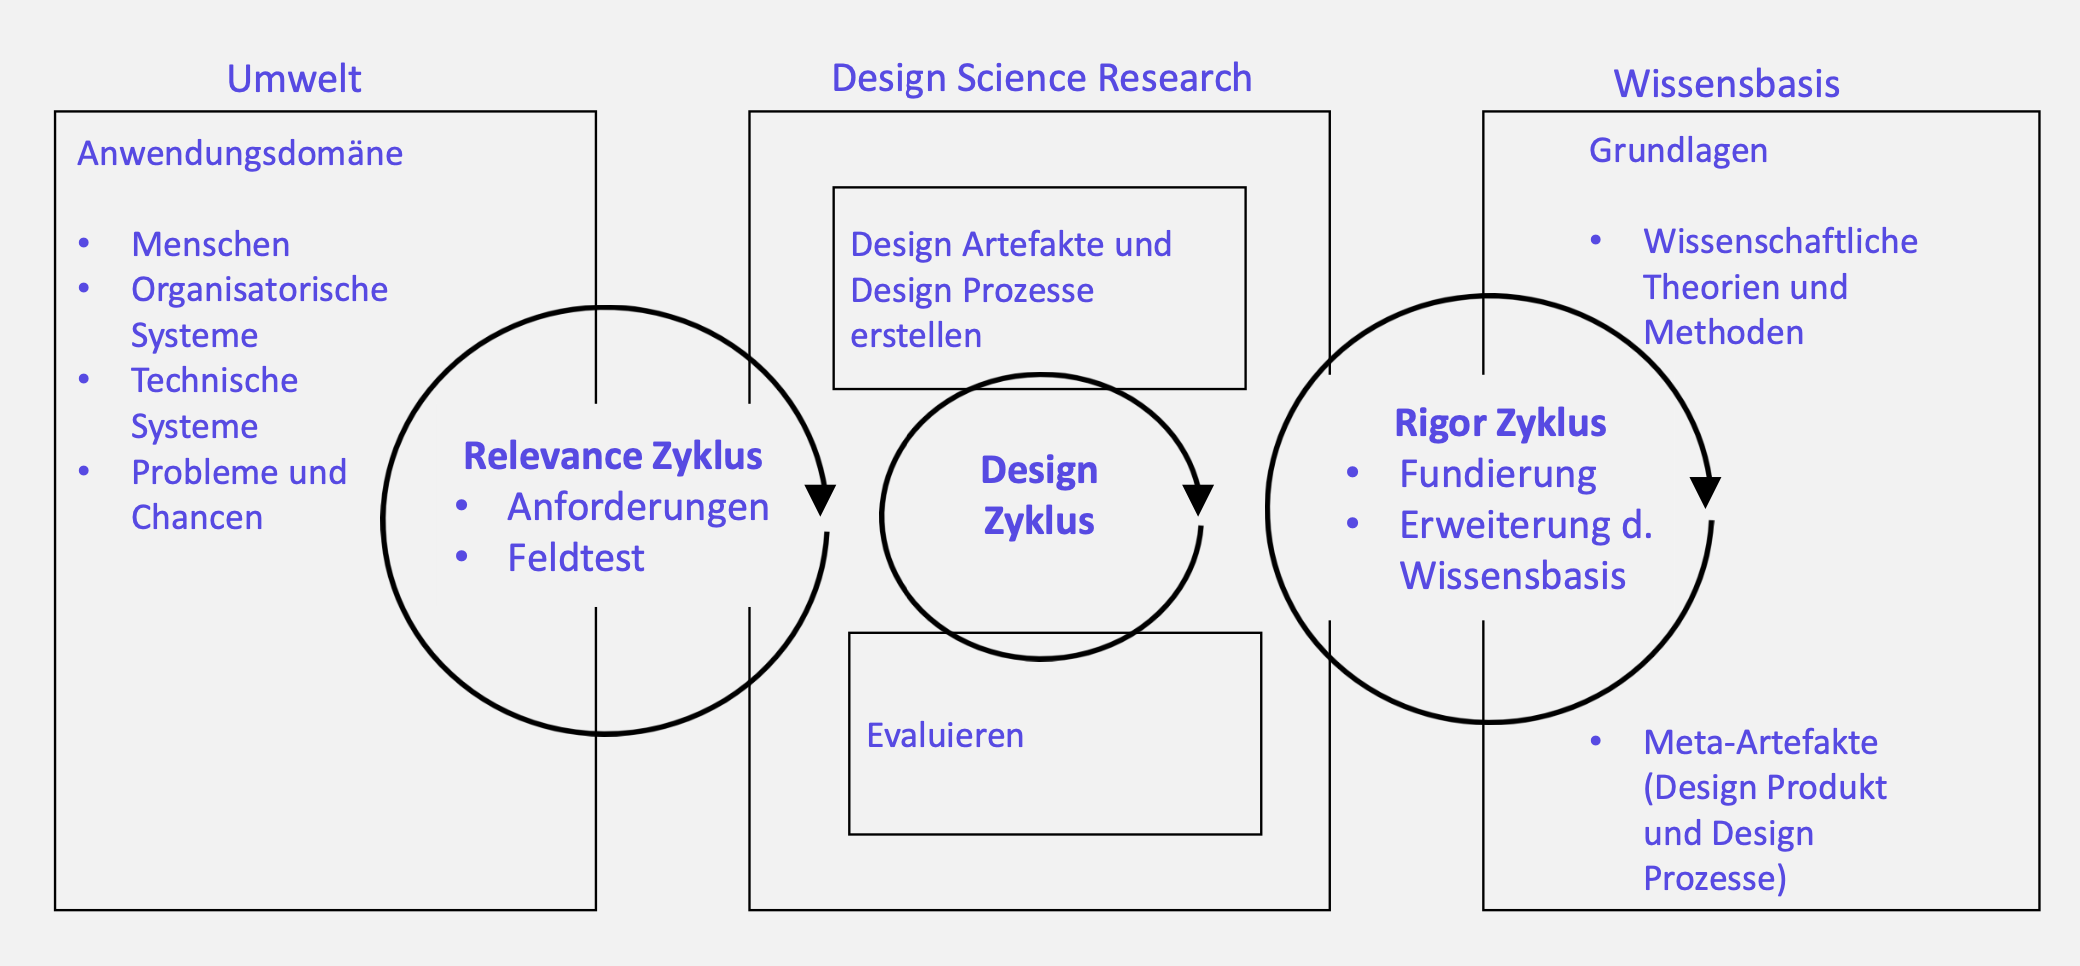
\includegraphics[width=1\linewidth]{images/Hevner.png}
    \caption[Design Science Research]{Design Science Research (eigene Darstellung, in Anlehnung an \parencite[88]{Hevner.2007})}
    \label{fig:DSR}
\end{figure}
Das Vorgehen der vorliegenden Arbeit basiert auf den eben genannten Zyklen.
\begin{itemize}
    \item \textbf{Relevance Zyklus:} \\
Hevner (2007) ist der Meinung, dass gute DSR Forschung mit der Identifizierung 
und Darstellung von Problemen in einem tatsächlichen Anwendungskontext beginnt.
Des Weiteren werden Akzeptanzkriterien für die Bewertung des Forschungsergebnisses definiert.
Abschließend werden in einem Feldtest die Ergebnisse evaluiert und bestimmt, ob 
eine weitere Iteration für die Anpassung der zuvor aufgestellten Anforderungen nötig ist. \parencite[89]{Hevner.2007}
Die vorliegende Arbeit stellt einen Ansatz für eine Identifikation des persönlichen Lernstils
eines Lernenden durch einen CA dar. Dazu wird ein Prototyp konstruiert.
Des Weiteren werden Bewertungskriterien aufgestellt, die prüfen, inwiefern die 
Interaktion mit dem Prototypen die Lernmotivation des Lernenden beeinflussen kann.
\item \textbf{Rigor-Zyklus:}\\
Eine umfangreiche Wissensbasis wissenschaftlicher Theorien und technischer Modelle stellen eine
Grundlage für Projekte der DSR Forschung. 
Der Rigor-Zyklus kann  
auf Wissen aus der Vergangenheit während des Forschungsprozesses 
zurückgreifen. Die Rigorosität der Forschung 
im DSR beruht auf der geschickten Auswahl und Anwendung geeigneter Theorien und Methoden. \parencite[90]{Hevner.2007}
Deshalb werden in der vorliegenden Arbeit relevante historische 
Theorien zur Lerntypologie vorgestellt,
um die ausgewählte Lerntypologie des Lernstils sowie das ausgewählte
ILS-Instrument von Felder und Soloman (1991), welches auf dem Lernstilmodell
 von Felder und Silverman (1988) basiert, zu begründen.
Für die Konzeption des Prototyps wird der aktuelle Stand der Forschung bezüglich der 
Themenkombination \glqq CA im Lehrformat\grqq{} sowie \glqq CA zur Identifikation des Lernstils\grqq{} untersucht.
Ferner werden für die Gestaltung des CAs Guidelines aufgestellt, welche sich 
auf identifizierte Aspekte der Wissensbasis zurückführen lassen.
Zur Ansammlung der benötigten Informationen wurde  
eine unsystematische Literaturanalyse genutzt.

\item \textbf{Design-Zyklus:}\\
Der Design Zyklus ist der Kernprozess eines DSR Forschungsprojekts. Dieser Zyklus stellt einen Ablauf 
von Forschungsaktivitäten dar, um Artefakte zu konstruieren und anschließend zu bewerten. \parencite[90 f.]{Hevner.2007}
Der Prototyp zur Identifikation des persönlichen Lernstils wird mithilfe einer Online-Umfrage evaluiert und weiterentwickelt.
\end{itemize}

\section{Aufbau der Arbeit}

Um den dargestellten Forschungsfragen nachzugehen, folgt die vorliegende Arbeit folgender Struktur:\\
Nach dieser Einleitung folgen \textbf{im 
zweiten Kapitel} die theoretischen Grundlagen des Lernens.
Es wird auf die Definitionen des Lernens, des digitalen Lernens und des selbstregulierten Lernens
eingegangen. Zur Beantwortung von RQ2 wird die Entstehung der Lernmotivation erläutert
sowie das ARCS-Modell zur Messung der Lernmotivation vorgestellt.
Für die Begründung der Wahl der Lerntypologie des Lernstils und des Modells von Felder und Silverman (1988), 
bedarf es vorerst einer Begriffsabgrenzung von Lerntypologien und eines Überblicks bekannter Modelle der Lerntypologien.
\textbf{Das dritte Kapitel} gibt eine Einführung in den Themenbereich der Chatbots.
Um die Chatbot-Begriffe abzugrenzen, folgen Definitionen  zum Chatbot,
zum Conversational Agenten
 und zum Virtual Companion.
Anschließend werden Informationen zum 
Natural Language Processing und zum Maschinellem Lernen aufgeführt, um 
zu klären inwiefern das Maschinelle Lernen Conversational Agents unterstützen. 
Zum Schluss des dritten Kapitels wird der aktuelle Stand der Forschung zu CAs dargestellt,
die eine mögliche Einschätzung vom Lernstil bei Lernenden untersucht haben oder in Lehrformaten
eingesetzt wurden. Dies dient der Erfassung der bestehenden Wissensbasis.
Das Kapitel zwei und drei stellen den theoretischen Teil der Arbeit dar. Die folgenden Kapitel
beziehen sich auf den Praxisteil der vorliegenden Arbeit.
\textbf{In dem vierten Kapitel} wird der Prototyp zur Identifikation des persönlichen Lernstils vorgestellt. 
Dabei wird zuerst auf das verwendete Framework Rasa eingegangen. Danach folgt die
Vorstellung des Prototyps, wobei vertieft auf 
die Dialog- und die Quiz-Spielgestaltung zwischen Lernendem und CA eingegangen wird.
\textbf{Das fünfte Kapitel} stellt die Evaluierung des Prototyps dar. 
Zuerst wird der Aufbau des Fragebogens erläutert. Anschließend folgt die Auswertung, welche nötig ist, um
RQ1 und RQ2 zu beantworten.
Abschließend folgt \textbf{im sechsten Kapitel} eine Zusammenfassung sowie 
eine kritische Würdigung des neu gewonnenen Wissens und
es wird ein Ausblick für weitere Forschungen aufgezeigt.

Bezogen auf die in Kapitel \ref{Vorgehensweise} beschriebene Vorgehensweise der Arbeit nach Hevner (2007),
spiegelt sich der Relevance Zyklus in der aufgeführten Problemstellung (vgl. Kapitel \ref{Problemstellung})
und in der Forschungsmotivation (vgl. Kapitel \ref{Forschungsmotivation}) wider.
Die unsystematische Literaturanalyse, 
welche erstens zur Analyse der Modelle der Lerntypologien, zweitens zum Stand der Forschung bezüglich 
bestehender CAs zur Lernstilklassifikation und CAs im Lehrformat, drittens zur
Aufstellung von Gestaltungsrichtlinien 
für den Prototypen (vgl. Kapitel \ref{AnalyseLernstilmodelle}, \ref{StandderForschung} und \ref{Gestaltungsrichtlinien})
genutzt wurde, repräsentieren wie die Studie zum Prototypen (vgl. Kapitel \ref{Kapitel5}) den Rigor Zyklus zur Generierung von neuem Wissen und neuen Erfahrungen.
Der Design Zyklus wird durch die Vorstellung und Evaluierung des Prototyps dargestellt (vgl. Kapitel \ref{VorstellungPrototyp} \& \ref{Kapitel5.2}).

\chapter{Theoretische Grundlagen des Lernens}
\chaptermark{Grundlagen}
Die Erkenntnisse des nachfolgenden Kapitels basieren vor allem 
auf der Psychologie, die einen breiten Forschungsbereich 
in Lerntheorien aufweist. Somit fallen in den nächsten Abschnitten 
oft Verweise auf psychologische Quellen.
Es folgt zuerst eine Erklärung von Begrifflichkeiten des Lernens (Kapitel \ref{BegriffLernen}),
eine Erläuterung zur Entstehung von Lernmotivation und eine kurze 
Einführung ins ARCS-Modell (Kapitel \ref{Lernmotivation}), da RQ2 
die Messung der motivationalen Anreize des 
Lernenden betrifft.
Anschließend folgt eine Begriffsabgrenzung von Lerntypologien (Kapitel \ref{Begriffsabgenzung}) sowie ein 
Überblick zu bekannten Modellen der Lerntypologien (Kapitel \ref{AnalyseLernstilmodelle}) gegeben wird.
Die Betrachtung der verschiedenen Modellen der Lerntypologien ist von Relevanz, um die ausgewählte Lerntypologie des Lernstils sowie  das ausgewählte
ILS-Instrument von Felder und Soloman (1991), welches auf dem Lernstilmodell von Felder und Silverman (1988) beruht, 
zu begründen (Kapitel \ref{AuswahlLernstilmodell}).
Dies ist wichtig, da für 
die Beantwortung von RQ1 ein geeignetes Messinstrument benötigt wird. 
    \section{Definitionen} \label{BegriffLernen}
        \subsection{Lernen} \label{Lernen}
            Lernen ist ein häufig vorkommender Begriff in der Alltagssprache und ein Grundbegriff der Pädagogik.
            Seine Vieldeutigkeit bestärkt sich durch das Vorkommen der hohen Anzahl verschiedenster Ansätze einer Begriffsdefinition.
            Eine eindeutige und präzise allgemeingültige Definition zu finden, ist schwierig. \parencite[103]{Treml.2004} 
            Doch Gemeinsamkeiten in den verschiedenen Definitionen bestehen darin, dass es beim Lernen darum geht, Wissen und Kenntnisse aufzubauen
            und dadurch Verhaltensänderungen durch Erfahrungen entstehen. \parencite[19]{marx.2006}
            In der vorliegenden Arbeit bezieht sich der Begriff Lernen besonders auf den Erwerb von Wissen und Kenntnissen.
            Wissen kann explizit erworben werden, welches 
            sich auf das allgemeine Lernen im Studium, in der Schule oder in einer Fortbildung bezieht und damit relevant für die vorliegende Arbeit ist.
            Treml und Becker (2004) bezeichnen das explizite Lernen \glqq als den bewussten Vorgang der Einprägung von Kenntnissen, der Aneignung und Entwicklung von Wissen, Erkenntnissen, Fertigkeiten, Gewohnheiten und Haltungen.\grqq{} \parencite[106]{Treml.2004} 
            Beim expliziten Lernen hat der Lernende die bewusste Absicht sich neues Wissen anzueignen. Seine volle Aufmerksamkeit ist auf das ihm klar definierte Lernobjekt gerichtet. \parencite[215]{RoehrSendlmeier.2016}
            Die Motivation ist eine notwendige Voraussetzung für jeden Wissenserwerb. \parencite[461]{Reinmann.1998} 
            Die Lernmotivation bekommt somit einen maßgeblichen Stellenwert im Lernprozess. Dahingehend wird seine Bedeutsamkeit in Teilabschnitt \ref{Lernmotivation} näher betrachtet.

        \subsection{E-Learning}
            Das E-Learning findet einen immer höheren Stellenwert in der Lehre und benötigt ein hohes Maß von selbstregulierten Handlungen in der Gestaltung des Lernprozesses. \parencite[34]{marx.2006} 
            E-Learning bezieht sich auf die Art und Weise, wie das Wissen bzw. die Informationen dargestellt, ausgetauscht und vermittelt werden können, und kann als 
            Oberbegriff für alle Varianten und Nutzung digitaler Medien zu Lehr- und Lernzwecken genannt werden. Als digitale Medien werden verschiedene Geräteklassen
            wie Desktop-Computer, Laptop, Tablet oder Smartphone mit entsprechender Periphere wie Beamer oder digitale Tafeln und Technik zur Aufnahme und Wiedergabe 
            von Medien bezeichnet. Sie unterstützen dabei Informationen digital zu speichern, zu verarbeiten und zu präsentieren, sodass an allen existierenden digitalen
            Artefakten gearbeitet werden kann und diese zwischen Menschen ausgetauscht werden können. \parencite[6]{Kerres.2013} 

        
        \subsection{Selbstreguliertes Lernen} \label{selbstgesteurtesLernen}
            Selbstorganisiert, selbstbestimmt, selbstgesteuert, autonom, nicht-organisiert, autodidaktisch, selbst gestalten oder selbst lernen sind teilweise auftretende Synonyme für selbststeuernd.
            Bezogen auf den Lernprozess muss der Lernende Aspekte wie:

            \begin{minipage}[t]{0.5\textwidth}
                \begin{itemize}
                \item das Ziel des Lernprozesses
                \item die Inhalte des Lernprozesses
                \item die Lernzeiten\\
            \end{itemize}
            \end{minipage}
            \hfill
            \begin{minipage}[t]{0.5\textwidth}
                \begin{itemize}
                \item den Lernort 
                \item die Art und Weise des Lernens  
                \end{itemize}
            \end{minipage}
            eigenständig steuern. Somit hängt diese zu steuernde Tätigkeit sowohl von den Anforderungen der jeweiligen Lernumgebung
            als auch von den Merkmalen der Lernenden ab.
            Der Selbststeuerungsgrad hängt davon ab, wieviel der Lernende von den oben genannten Aspekten ohne Fremdeinwirkung selbst zu steuern hat. \parencite[14 f.]{Dietrich.2007} \parencite[195]{Cress.2000}
            Somit fordert das selbstregulierte Lernen vom Individuum, sein Lernen und Denken eigenständig zu regulieren und zu bestimmen. \parencite[45]{Groß.2017} 
            Das selbstregulierte Lernen ist ein allgemeines großes Motivationsproblem (vgl. Kapitel \ref{Problemstellung}).
            Daher soll mithilfe des Prototyps der Arbeit untersucht werden, inwiefern die Motivation des Lernenden bei der Unterstützung der Gestaltung des Lernprozesses beeinflusst werden kann.

        
    \section{Lernmotivation} \label{Lernmotivation}
    Im psychologischen Sinne bezeichnet Heckhausen (1989) Motivation \glqq als eine Sammelbezeichnung für verschiedene Prozesse und Effekte, deren gemeinsamer Kern darin besteht, dass ein Individuum
    sein Verhalten um der erwarteten Folgen willen auswählt und hinsichtlich Richtung und Energieaufwand steuert\grqq{}. \parencite[10]{heckhausen.1989} 
    Im Allgemeinen ist die Motivation die Bereitschaft in einer konkreten Situation eine bestimmte Handlung mit einer bestimmten Intensität durchzuführen. \parencite[4]{tischner.2007} 
    Somit ist die Motivation bestimmend für die Dauer und die Intensität der Lernbereitschaft und den Erfolg beim Lernen. \parencite[44]{Grotian.1999}
    Die vorliegende Arbeit beschäftigt sich mit der Lernmotivation bezüglich des expliziten Lernens und des selbstregulierten Lernens.
    
    \subsection{Modell zur Lernmotivation}
    Das folgende Modell beschreibt einen theoretischen Ansatz, auf welche Art und Weise das selbstregulierte Lernen von Einflussgrößen bestimmt wird und welche Auswirkungen es mit sich zieht.
    
    \begin{figure}[H]   
        \centering
        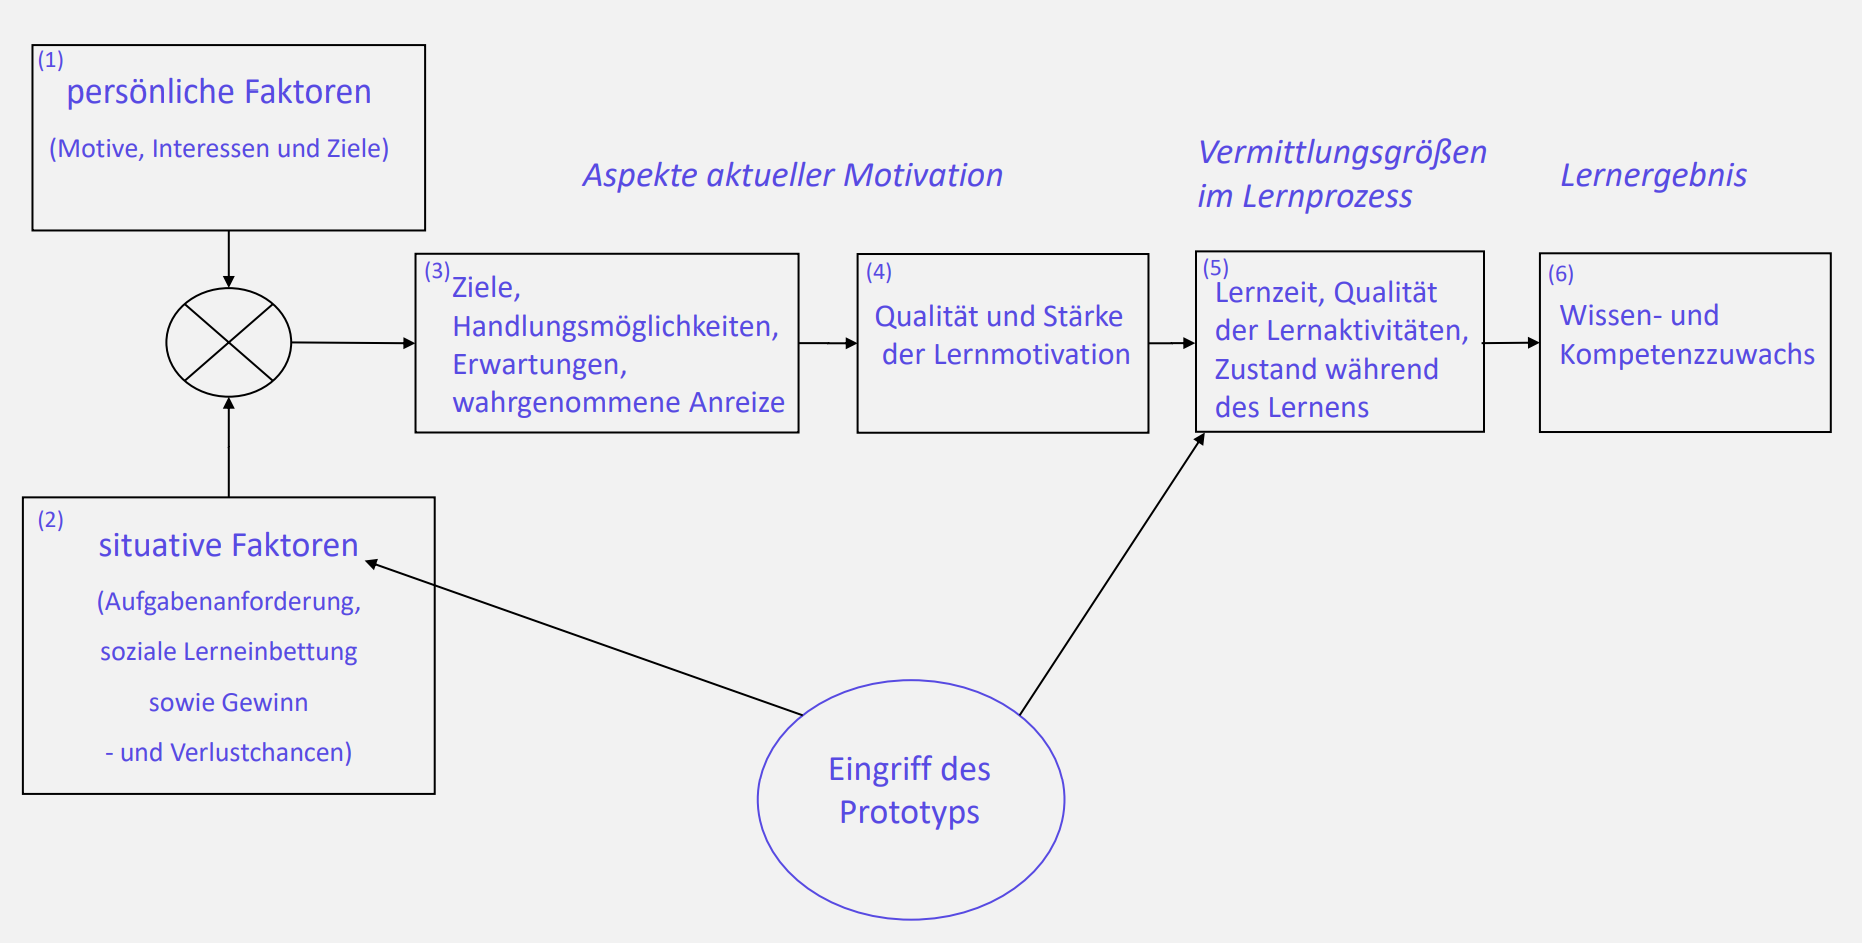
\includegraphics[width=0.6\linewidth]{images/Rahmenmodell_Lernmotivation.png}
        \caption[Modell zur Lernmotivation]{Modell zur Lernmotivation (eigene Darstellung, in Anlehnung an \parencite{rheinberg.2000})}
        \label{fig:Rahmenmodell zu Bedingungen und Auswirkungen von Lernmotivation}
    \end{figure}
    
    In diesem Modell ist erkennbar, dass das motivierte Verhalten sich durch eine Wechselwirkung von persönlichen Faktoren (Box 1) wie Motive, Interessen und Ziele und den situativen Faktoren (Box 2) bedingt.
    Die situativen Faktoren umfassen neben der Struktur und Schwierigkeit der Aufgabenstellung, welche abhängig von den 
    Kompetenzen des Lernenden sind,
    die allgemeine Lernsituation des sozialen Umfeldes (alleine lernen vs. lernen innerhalb einer Gruppe)
    sowie die potentiellen Gewinn- und Verlustchancen, die der Lernende erwarten könnte. Mögliche Gewinnchancen können sein:
    
    \begin{minipage}[t]{0.5\textwidth}
    \begin{itemize}
        \item die eigenen Fähigkeiten kennen zu lernen und sie ggf. zu verbessern
        \item gute Noten zu erreichen\\
    \end{itemize}   
    \end{minipage}
    \hfill
    \begin{minipage}[t]{0.5\textwidth}
        \begin{itemize}
        \item das Lernen über etwas, das man interessant findet
        \item Lob von relevanten Akteuren \\
    \end{itemize}
\end{minipage}

    In welcher Weise sich jeder genannte situative Faktor auf die Lernmotivation des Lernenden auswirkt, hängt von dessen persönlichen Charakterzügen ab. \parencite[83]{rheinberg.2000} 
    Der Prototyp dieser Arbeit greift in den situativen Faktor ein. 
    Er soll als Unterstützung für den Lernenden dienen, 
    indem er die Aspekte des situativen Faktors positiv beeinflusst.
    Zum Beispiel kann der Prototyp den Lernenden dazu
    ermutigen, mehr über seine eigene Art und Weise des Lernens zu erkunden sowie seine Stärken und Schwächen zu 
    identifizieren und dadurch einen höheren Lernerfolg erzielen.
    Darüber hinaus kann der Prototyp 
    als soziale Bezugsperson dienen und ein virtueller Begleiter für den Lernenden werden.
    Je positiver die Einschätzung über die Erwartungen und Anreize, die der Lernende in der Situation wahrnimmt, ausfällt, desto höher ist die Lernmotivation.
    Denn ein gewünschter Kompetenzzuwachs stellt sich ein und die oben genannten Gewinnchancen werden erreicht. 

    Die Interaktion zwischen Personen- und Situationsmerkmalen beeinflussen die Zielsetzung, die Erwartungen des Lernenden und die Anreize, die er in dieser Situation für möglich hält (Box 3). Diese Variablen bestimmen ihrerseits sowohl die Stärke als auch die Qualität der Lernmotivation (Box 4). 
    Also ist die Motivationsstärke dafür entscheidend, wie gut sich Lerntätigkeiten (z.B. 
    das Durcharbeiten eines Textes, vorausgesetzt das Thema ist für den Lernenden interessant), gegenüber konkurrierenden Tätigkeiten (z.B. ein Kinobesuch) durchsetzen können. \parencite[20 f.]{marx.2006} 
        
    Lernmotivation an sich kann keine Lernergebnisse erzeugen. Box fünf stellen Variablen dar, die vermitteln, welchen Einfluss die Lernmotivation auf das Lernen haben kann.
    Im Fall des selbstregulierten Lernens, bei dem der Lernende einen hohen Freiheitsgrad
    in der Art und Weise des Lernens hat, stellen die Zeit und die Art der Lernaktivität eindeutige Variablen dar. \parencite[84]{rheinberg.2000} 
    Der Prototyp der vorliegenden Arbeit kann durch die Bestimmung des individuellen Lernstils des Lernenden 
    eine Tendenz zur richtigen Wahl bezüglich der Art und Weise der Lernaktivität geben. Wird zum Beispiel 
    der Lernstil visuell beim Lernenden identifiziert, kann der Lernende vorerst den Lehrstoff mithilfe
    von visuellen Materialien vertiefen.
    Eine weitere Variable ist der Zustand des Lernenden während des Lernens, der das Lernergebnis beeinflusst.
    Dabei bezieht sich diese Variable auf die physiologische und psychologische Aktivierung und Konzentration des Lernenden während des Lernens. \parencite[84]{rheinberg.2000} 
    Abschließend kann das Lernergebnis den Motivationsprozess weiter fördern, indem der Lernende den erlebten Lernerfolg auf zukünftige Lernsituationen überträgt. Dazu muss der Lernende seinen Lernzuwachs wahrnehmen, indem 
    er die neu gewonnene Leistung mit seinen eigenen vorangegangenen Leistungen vergleicht. \parencite[21]{marx.2006} 

        \subsection{Das ARCS-Modell} \label{Kap2ARCS}
        Aus dem obigen Abschnitt ist deutlich geworden, dass die jeweilige Motivation sowohl zum einen von Merkmalen, Charakteristika und Motiven einer Person abhängt als auch von situativen Faktoren
        beeinflusst wird. 
        Dieses Teilkapitel stellt das ARCS-Modell von Keller (1984) vor, womit die Lernmotivation des Lernenden gemessen werden kann:
        

        \begingroup
        \footnotesize    
        \useunder{\uline}{\ul}{}
        \begin{longtable}{|m{5cm}|m{10cm}|}
        \hline     
        \rowcolor[HTML]{EFEFEF}                                         
        \centering \textbf{Dimension} & \centering \arraybackslash \textbf{ Erläuterung} \\ 
        \hline  \hline 
        Attention (dt. Aufmerksamkeit) & Diese Kategorie bezieht sich auf das Erfassen des Interesses sowie auf die Neugier des Lernenden.
         \\ \hline \hline
        
         Relevance (dt. Relevanz) & Hierbei handelt es sich um die Vermittlung und Bedeutung des Lehrstoffs. Der Lernende soll eine Vorstellung davon bekommen, inwiefern die gezeigten 
         Inhalte mit wichtigen persönlichen Zielen oder Motiven zusammenhängen und somit für ihn eine Relevanz darstellen. 
         \\ \hline \hline

         Confidence (dt. Zuversicht) & Dieser Aspekt meint die Unterstützung der Erfolgszuversicht des Lernenden sowie die Maximierung der Erfolgserwartungen, sodass 
         der Lernende seine gesteckten Ziele aus eigener Anstrengung erreicht. 
         \\ \hline \hline

         Statisfaction (dt. Zufriedenheit) & Die Anstrengung des Lernenden führt zum gewünschten Erfolg und er bleibt motiviert.
         Die Motivation kann dabei aus extrinsischen und intrinsischen Faktoren entstehen. 
         \\ \hline \hline


    \caption[Keller (1984): ARCS-Dimensionen]{Keller (1984): ARCS-Dimensionen (eigene Darstellung, in Anlehnung an \parencite[45 f.]{keller_2010})} 
    \label{tab:/ARCS_Dimensionen_Keller} 
    \end{longtable}
    \endgroup  

       \textbf{Intrinsische und extrinsische Lernmotivation}

        Die Begriffe intrinsische und extrinsische Motivation werden häufig benutzt, allerdings besteht keinerlei Einigkeit darüber, was damit gemeint ist. 
        Möglich ist die folgende Erklärung.
        Aus dem Englischen abgeleitet, bedeuten die beiden Begriffe \glqq innen\grqq{} (engl. intrinsic) und \glqq außen\grqq{} (engl. extrinsic). Die intrinsische Motivation bezieht sich 
        auf Handlungen, die aus der Freude heraus selbst ausgeführt werden. 
        Dazu können sportliche Aktivitäten wie Bergsteigen, Laufen oder auch Aktivitäten wie das Lesen oder Malen gehören, denn der
        Spaßfaktor, welcher während der Tätigkeitsausführung durchlebt wird, ist hoch. 
        Im Gegensatz dazu werden extrinsische Handlungen wegen der erwarteten Folgen ausgeführt. Zum Beispiel kann beim Lernen für eine Klausur das Erreichen einer guten Note, das Abschließen eines Studienmoduls
        oder die Erfüllung der Erwartungen der Eltern den Zweck der Handlungsausübung darstellen. \parencite[5 f.]{Zander2018}

        Das ARCS-Modell dient als Messinstrument, um die Lernmotivation der Probanden in der Studie, welche in Kapitel \ref{Kapitel5.1} aufgeführt wird, zu messen.
        Dies ist von Relevanz, um RQ2 zu beantworten.

    \section{Begriffsabgrenzung von Lerntypologien} \label{Begriffsabgenzung}
    Die Forschung befasst sich mit dem Versuch auf der Basis von verschiedenen theoretischen Modellen mithilfe von Testverfahren, die Art und Weise des Lernens eines Menschen zu klassifizieren, damit dieser dann die Möglichkeit hat, speziell auf seinen Typus
    abgestimmte Lernmethoden zu nutzen und so sein Lernen zu optimieren. Von dieser verlockenden Idee sind viele praktisch tätige Pädagogen überzeugt, die in ihrer täglichen Arbeit interindividuelle Unterschiede bei den Herangehensweisen 
    und Arbeitsweisen der Lernenden beim Lernen feststellen. \parencite[13f.]{Martin.2012}
    Allerdings gibt es keine Einigkeit darüber, welche Verhaltensweisen oder charakteristischen Lernmerkmale in der Klassifikation zur Bestimmung des individuellen Lerntypus miteinbezogen werden sollen. Diese Unstimmigkeit spiegelt sich 
    in der Vielfalt an Ansätzen von theoretischen Modellen  wider und erschwert somit eine eindeutige Abgrenzung der Begrifflichkeiten: Kognitiver Stil, Lernstil, Lernorientierung, Lernpräferenz,
    Lerntyp, Lernstrategie und Lerntaktik. \parencite[9]{Zeiter.2011} \parencite[365]{Cress.2006}
    Creß (2006) unterscheidet einige der eben aufgezählten theoretischen Begrifflichkeiten nach einem Zusammenhang zwischen dem in einer konkreten Situation beobachtbarem Verhalten 
    zu einem situationsübergreifenden Verhalten sowie personenbezogenen Merkmalen. \parencite[365]{Cress.2006} 
    Die nachfolgende Abbildung stellt eine grobe Übersicht der Idee der Unterscheidungsmerkmale dar.
    
    \begin{figure}[H]
        \centering
        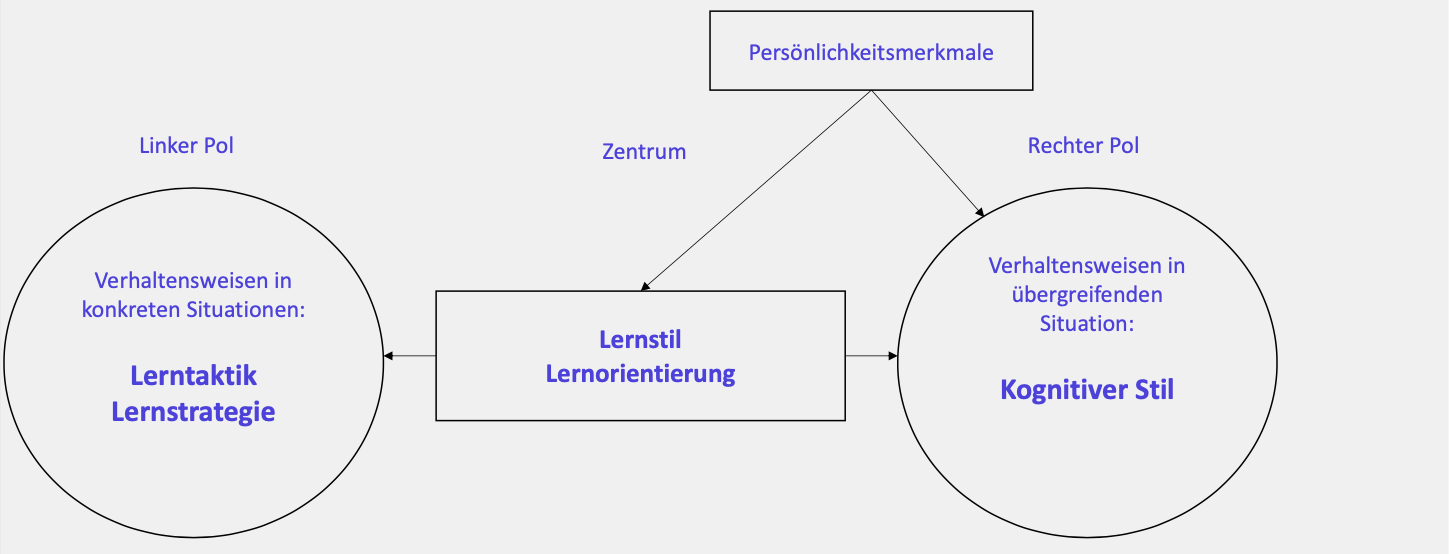
\includegraphics[width=0.8\linewidth]{images/AbgrenzungTheoretischerKonzepte.png}
        \caption[Überblick: Begrifflichkeiten theoretischer Lerntypologien]{Überblick: Begrifflichkeiten theoretischer Lerntypologien (eigene Darstellung, in Anlehnung an \parencite[11]{Zeiter.2011})}
        \label{fig:Überblick Begrifflichkeiten theoretischer Modelle}
    \end{figure}

    Die dargestellte Abbildung zeigt zwei Pole auf, wodurch die Kontradiktion der Verhaltenssituationen verdeutlicht werden soll.
    Der linke Pol steht für die Verhaltensweisen in einer konkreten Situation und der rechte Pol stellt die Verhaltensweisen in übergreifenden Situationen inklusiver Persönlichkeitsmerkmalen dar.
    Die Lerntaktik und Lernstrategie stellen den situationsnahen Pol dar, der Kognitive Stil bildet den anderen Pol. Der Lernstil und die Lernorientierung sind in dem Zentrum der Pole zu finden und 
    zeigen charakteristische Züge. Diese bilden eine Schnittmenge mit den persönlichen Merkmalen, da sie persönliche Charakterzüge aufweisen.
    Im Folgenden werden die einzelnen theoretischen Begrifflichkeiten näher erläutert.

        \textbf{Lernstrategie - und taktik}

            Wild (2006) definiert Lernstrategien allgemein als \glqq jene Verhaltensweisen und Kognitionen, die vom Lernenden aktiv zum Zweck
            des Wissenserwerbs eingesetzt werden.\grqq{} \parencite[427]{Wild.2006} 
            Neben der kognitiven Handlung werden auch Handlungen zur Beeinflussung des motivationalen und affektiven Zustands (z.B. Selbstbelohnung) gezählt. \parencite[5]{Martin.2012} 
            Streblow und Schiefele (2006) fassen folgende gemeinsamen Merkmale in den bestehenden Definitionen der Lernstrategie zusammen:
        
            \begin{enumerate}
                \item Lernstrategien enthalten eine Reihe von effizienten Lerntechniken, welche die Methoden darstellen, die dem Lernenden helfen, die Aufnahme und Verarbeitung des neuen Wissens zu erleichtern. 
                            Beispielsweise ist das Schreiben von Karteikarten (Lerntechnik) für das Auswendiglernen (Lernstrategie) eine oft verbreitete Technik. 
                \item Lernstrategien werden situationsangepasst, zielbewusst und flexibel eingesetzt.
                \item Lernstrategien laufen automatisiert ab. 
                \item Lernstrategien haben das Potenzial bewusstseinsfähig zu werden, sodass die Person die verwendete Lernstrategie soweit verinnerlicht, dass die Handlungen nicht mehr bewusst initiiert und gesteuert werden müssen.
            \end{enumerate} 
            Darüber hinaus werden Lernstrategien in metakognitive und kognitive Strategien sowie in das Ressourcenmanagement unterschieden. \parencite[353]{Streblow.2006} 
            Auf diese wird im späteren Verlauf der Arbeit weiter eingegangen.
            Lernstrategien können gelernt und modifiziert werden und somit der Situation angepasst werden, deshalb beschreiben sie den situationsnahen Pol. \parencite[142]{Looss.2007}
       

        \textbf{Lernstil \& Lernorientierung}

        Der Lernstil einer Person beschreibt weniger die Informationsverarbeitung im Allgemeinen, sondern mehr das individuelle und typische Verhaltensmuster, das eine Person bei Lernaufgaben situationsübergreifend zeigt.
        Diese kognitive und affektive Verhaltensweise der Person stellt ebenfalls charakteristische Züge der Person dar, welche sich als relativ stabil einschätzen lassen. \parencite[142]{Looss.2007}\parencite[58]{Groß.2017}\parencite[365]{Cress.2006} \\
        Als Lernorientierung wird die Art und Weise bezeichnet, in der die Charakterzüge der Person und die Merkmale der Situation ineinander greifen. \parencite[142]{Looss.2007}
        Beide Typologien sind daher dem Zentrum der Abbildung \ref{fig:Überblick Begrifflichkeiten theoretischer Modelle} zuzuordnen.

    
        \textbf{Kognitiver Stil}

        Der Kognitive Stil ist gegenüber der Lernorientierung und dem Lernstil in der Art und Weise der Informationsverarbeitung einer Person allgemeiner gefasst
        und sind daher dem rechten Pol in der Abbildung \ref{fig:Überblick Begrifflichkeiten theoretischer Modelle} zugeordnet. 
        Die allgemeingültige Art des kognitiven Stils zeigt sich als ein gewohnheitsmäßiges und situationsübergreifendes Verhalten und wird als Persönlichkeitsmerkmal gekennzeichnet.\parencite[365]{Cress.2006} 
        Allerdings sind die Konzepte zum Kognitiven Stil nicht empirisch und theoretisch überzeugend. \parencite[339]{tiedemann.2001}
        
        \textbf{Lerntyp \&  Lernpräferenz}

        Einige Autoren verwenden den Begriff Lerntyp auch im Sinne der Lernpräferenz. Aus einer bestimmten Lernpräferenz lassen sich Lerntypen ableiten. \parencite[372]{Cress.2006} 
        Zudem ist eine sehr bekannte verbreitete These, dass sich Lerntypen auf der Basis von Sinneskanälen unterscheiden lassen.
        Allerdings fehlt es an logischer und empirischer Evidenz diese These zu beweisen.
        Dennoch genießt diese Lerntypentheorie, welche auf den Autor Vester (1998) zurückzuführen ist, ein hohes Maß an Popularität. \parencite[144]{Looss.2007} \nocite{Vester.1998}
        Vester (1998) behauptet eine Abhängigkeit des individuellen Lernerfolgs und der persönlichen Lernpräferenz von unterschiedlichen Wahrnehmungskanälen zu erkennen. Daraufhin definiert er vier 
        unterschiedliche Lerngruppen und unterscheidet zwischen dem visuellen, optischen, haptischen und intellektuellen Lerntyp. \parencite[144]{Looss.2007} \parencite[17]{Schrader.2008} \parencite[372]{Cress.2006} 
        Der Begriff der Lernpräferenz wird beispielsweise oft in Verbindung mit den Ansätzen von Vester (1998) und Neber (1994) gebracht. Bei Neber (1994) wird nach der Präferenz für autonomes Lernen 
        oder Lernen in der Gruppe unterschieden. \nocite{Neber.1994}
        Allerdings sind die Versuche, Lerntypen über Lernpräferenzen zu ermitteln theoretisch wenig fundiert. \parencite[375]{Cress.2006}  
            
        Zusammenfassend ist an dieser Stelle zu erwähnen, dass die Lerntypologien: Kognitiver Stil, Lerntyp und Lernpräferenz aufgrund von zu wenig fundierter Überzeugungskraft nicht 
        als weitere mögliche Typologie in Frage kommen und deshalb nicht für die Begründung der ausgewählten Lerntypologie beachtet werden.
        
        \section{Analyse historischer bekannter Modelle der Lerntypologie} \label{AnalyseLernstilmodelle}

    Die  Forschungsansätze der Lernstrategie und -stiltheorien nehmen ihren Verlauf bis zur Antike. 
    So folgt eine Einschränkung auf die theoretischen Konzeptionen der letzten 50 Jahre in der Geschichte. Es herrschen zwei dominierende Forschungsstränge: 
    \textbf{\glqq Approach to Learning-Ansätze\grqq{}} und \textbf{\glqq Kognitionspsychologische-Ansätze\grqq{}}.
    Der  \textbf{ Approach to Learning (ATL)} Ansatz beschreibt das unterschiedliche Lernverhalten der Menschen. Dieses unterschiedliche 
    Lernverhalten kann in verschiedenen Situationen beobachtet werden und weist einen
    Bezug zu den jeweiligen Persönlichkeitszügen des Lernenden auf. 
    Die Identifikation mit seinen charakteristischen Merkmalen steht im Vordergrund. 
    Die  \textbf{kognitiven Ansätze} beziehen sich hauptsächlich auf die Frage, wie der Lernprozess allgemein funktioniert und optimiert werden kann. Dabei wird die Vorgehensweise von Informationsaufnahme über die
    Verarbeitung bis hin zur Speicherung sowie den Möglichkeiten zur Beeinflussung dieses Prozesses untersucht. In vielen nachfolgenden Konzepten wird keine klare Trennung bezüglich der Methoden und Ziele der beiden 
    Forschungsrichtungen geschaffen. \parencite[8]{Martin.2012} 
    Die nachfolgende Abbildung zeigt wichtige Vertreter der Lernstrategie und -stilforschung in chronologischer Abfolge. Anschließend werden die Grundgedanken der Befunde kurz erläutert, um 
    die geeignete Lerntypologie und das geeignete Modell zu begründen, welche für die Beantwortung von RQ1 relevant sind. 

    
    \begin{figure}[H]
        \centering
        \includegraphics[width=0.8\linewidth]{images/timeline.png}
        \caption[Timeline: Vertreter von Lerntypologie-Modellen]{Timeline: Vertreter von Lerntypologie-Modellen (eigene Darstellung)}
        \label{fig:Timeline: Vertreter von Lerntypologie-Modellen}
    \end{figure}

        \subsection{Approach to Learning Ansätze} \label{ATL}
        \textbf{Marton \& Säljö (1976)} entdeckten zwei grundlegende Herangehensweisen an das Lernen: \textbf{\glqq Surface-Approach\grqq{} } (dt .Oberflächenverarbeitung) und 
        \textbf{\glqq Deep-Approach\grqq{} } (dt. Tiefenverarbeitung). \nocite{Marton.1984}
        Die erste Kategorie beschreibt eine auf Wiederholung und Auswendiglernen ausgerichtete Herangehensweise, die  weniger am tiefen Verstehen und mehr an der exakten Wiedergabe von losen Fakten interessiert ist.
        Die zweite Kategorie zeigt ein Verhaltensmuster, wodurch der Lernende Zusammenhänge und Querverbindungen zu seinem Vorwissen versucht zu verknüpfen. Er ist an dem Verstehen der Informationen interessiert. \parencite[8 f.]{Martin.2012}\parencite[366]{Cress.2006}\parencite[145 f.]{Looss.2007}
        
        Unabhängig von Marton \& Säljö (1976), jedoch zu derselben Zeit, identifiziert der Brite \textbf{Pask (1976)} zwei Lernstrategien \textbf{\glqq holistic\grqq{}} (dt. ganzheitlich) und \textbf{\glqq serialistic\grqq{}} (dt. serialistisch). Dabei bezeichnet er Personen, welche die holistic Strategie wiederholt anwenden als \textbf{\glqq Comprehension Learner\grqq{}}. 
        Dieses Lernverhalten zeichnet sich durch eine globale Lerneinstellung aus. Das Lernen ist reich an Ankedoten, Illustrationen und Analogien.
        Anwender der serialistic Strategie werden als \textbf{\glqq Operating Learner\grqq{}} beschrieben. Dieses Lernverhalten ist durch die sukzessive Bearbeitung des Lernstoffes geprägt. Der Lerner arbeitet kleinschrittig und 
        beginnt beim Detail, bevor er zum Gesamten übergeht. Pask
        (1976) ist ein Befürworter eines flexiblen Lernverhaltens und bezeichnet Personen, die
        je nach Aufgabenstellung entweder die holistic oder serialistic Strategie anwenden als
        \textbf{\glqq Versatile Learner\grqq{}}.
        Die beiden Lernstile Comprehension Learner und Operating Learner sind mit den Dimensionen von Surface- und Deep-Aproach vergleichbar.
        \parencite[9]{Martin.2012}\parencite[369]{Cress.2006}\parencite[12 f.]{Thielke.2003} 

        Gestützt auf die Untersuchungen von Marton \& Säljö (1976) und Pask (1976), die als Orientierungsansätze für die weitere Forschung gelten, unternahm die britische Forschungsgruppe um \textbf{Entwistle \& Ramsden (1983)} den Versuch anhand von faktoranalytischen Methoden\footnote{Faktoranalysen gehören zu den Methoden der multivarianten Statistik und dienen dazu, aus einer empirischen Beobachtung von vielen verschiedenen manifesten Variablen auf wenige zugrunde liegende latente Variablen zu schließen. Vgl. \url{https://eric-klopp.de/texte/explorative-faktorenanalyse.php}, aufgerufen am 04.11.2021},
        einen quantitativen Fragebogen zur 
        Erfassung der Herangehensweisen an das Lernen im Sinne der obigen ATL-Dimensionen zu erstellen. Der \textbf{\glqq Approaches to Studying\grqq{}  (ASI)}  Fragebogen von Entwistle \& Ramsden (1983) sollte die Erhebung 
        des Lernverhaltens von größeren studentischen Stichproben ermöglichen. Die Auswertung der Pilotstudie ergab eine systematische Verknüpfung von Lernmotivation und Lernverhalten. \parencite[9]{Martin.2012}\parencite[368 f.]{Cress.2006} 

        Gleichzeitig entwickelte die australische Forschergruppe um \textbf{Biggs (1987)} einen ähnlichen Ansatz zu den oben genannten Lernorientierungen. \nocite{Biggs.1987}
        Er forderte die Verknüpfung von Lernmotivation und spezifischem Lernverhalten zu einer distinkten Herangehensweise an eine Lernaufgabe und stellte dabei drei Dimensionen fest. Er unterschied zwischen 
        dem \textbf{\glqq Surface-Approach\grqq{}}, dem \textbf{\glqq Deep-Approach\grqq{}} und dem \textbf{\glqq Achieving-Approach\grqq{}} (dt. Erfolgreicher-Ansatz).
        Diese Ansätze hat er in seinem  \textbf{\glqq Study Process Questionnaire\grqq{} (SPQ)} mit je einer motivationalen und einer strategischen Skala abgebildet. \parencite[10]{Martin.2012}\parencite[367 ff.]{Cress.2006} 
        Der Surface- und Deep-Approach beziehen sich auf die Art der Auseinandersetzung mit dem Lernstoff und entsprechen somit den Konzepten von Marton \& Säljö (1976). \parencite[383]{Wild.2000}
        Der Achieving-Approach wirkt sich nicht sehr stark auf den Lernprozess aus, sondern dient der Strukturierung der räumlichen und zeitlichen Rahmenbedingungen und ähnelt somit dem Konzept des Versatilen Lerners von Pask (1976). \parencite[15]{Thielke.2003}
        
        Aufgrund einer hohen Anzahl an Studienabbrüchen in der schwierigen Ingenieurausbildung in den USA entwickelten 
        \textbf{Felder und Silverman (1988) (FS)} ein theoretisches Lernstilmodell speziell für diese Ausbildung. Das FS-Modell klassifiziert 
        auf einer Skala, in welcher Form Lernende Informationen aufnehmen. \parencite[21 f.]{Felder.1995} \parencite[674]{Felder.1988}
        \textbf{Felder und Soloman (1991)} entwickelten ein Instrument namens \textbf{\glqq Index of Learning Styles\grqq{} (ILS)} zur Bewertung dieses 
        Lernstilmodells. \parencite[2]{Felder.2002}
        Folgende vier
        Lernstile\footnote{Die Dimensionen induktiv/deduktiv wurden entfernt und die Dimensionen visuell/auditiv wurde in visuell/verbal geändert. \parencite[1 f.]{Felder.2002}} werden definiert: 
        
        \begingroup
            \footnotesize    
            \useunder{\uline}{\ul}{}
            \begin{longtable}{|m{3cm}|m{12cm}|}
            \hline     
            \rowcolor[HTML]{EFEFEF}                                         
            \centering \textbf{Dimension} & \centering \arraybackslash \textbf{ Erläuterung} \\ 
            \hline  \hline 
            Sensorisch/ intuitiv &  \textbf{Sensorische Lerner} bedienen sich detailreicher Fakten, Daten und Informationen. Sie haben eine sorgfältige und fleißige Arbeitsstruktur sowie sie die Lernstrategie des Auswendiglernens nutzen. Um wissenschaftliche Methoden korrekt anzuwenden, fordern sie in diese eine gute Einführung und lehnen Aufgabengebiete, die in Lehreinheiten nicht behandelt wurden, ab. \textbf{Intuitive Lerner} zeigen ein gegensätzliches Verhalten zum sensorischen Lerner auf. Sie versuchen 
            Auswendiglernen und Wiederholungen zu umgehen. Des Weiteren bevorzugen sie Theorien und Konzepte, um eigenständig
            Schlüsse aus den Informationen zu ziehen sowie von komplexeren Aufgaben herausgefordert zur werden. 
             \\ \hline \hline
            Visuell/ verbal & \textbf{Visuelle Lerner} bevorzugen die Präsentation von Informationen in Bildern, Diagrammen, Flussdiagrammen, Zeitleisten, Filmen und Demonstrationen. \textbf{Verbale Lerner} ziehen schriftliche oder gesprochene Erklärungen vor. 
            \\ \hline \hline
            Aktiv/ reflektiv &  \textbf{Aktive Lerner} bevorzugen in Lernsituationen, die ihnen ermöglichen, etwas Aktives zu tun, zum Beispiel eine Teilnahme an einer Diskussion über das Thema oder jemandem etwas zu erklären.
            Sie bevorzugen Gruppenarbeit. \textbf{Reflektive Lerner} benötigen eine Gelegenheit, in der sie vorerst über die Informationen nachdenken können. Sie bevorzugen es alleine zu arbeiten.
            \\ \hline \hline
            Sequentiell/ global & \textbf{Sequentielle Lerner} lösen Probleme Schritt für Schritt, damit sie den klaren linearen Zusammenhang erkennen können. Durch diesen logischen Aufbau können sie mehr Informationen aufnehmen. \textbf{Globale Lerner} können Probleme schnell anhand des Gesamtbildes lösen. Allerdings haben sie Probleme, Einzelheiten ihres Denkprozesses zu erläutern.
            \\ \hline \hline
        \caption[Felder und Silverman (1988): FS-Dimensionen]{Felder und Silverman (1988): FS-Dimensionen (eigene Darstellung, in Anlehnung an \parencite[22 ff.]{Felder.1995})} 
        \label{tab:/ILS-Dimensionen} 
        \end{longtable}
        \endgroup  
        
        Im Folgenden wird der zweite Forschungsstrang vorgestellt, um die ausgewählte Lerntypologie zu begründen.

        \subsection{Kognitionspsychologische Ansätze }
        In den 1980er Jahren
        entwickelten \textbf{Weinstein und Mayer (1986)} in den USA  einen neuen Forschungsstrang, der das Lernen explizit als Informationsverarbeitungsprozess verstand.
        Die Beeinflussung des  Enkodierungsprozesses\footnote{Der Enkodierungsprozess ist die Übersetzung der neuen Sinneseindrücke in neuronalen Code, sodass das Gehirn die neuen Informationen verarbeiten kann. \parencite[178]{berting.2011}}
        beim Erwerb neuer Informationen war die Grundlage dieses Ansatzes. Der Prozess kann in \textbf{Selektion}, \textbf{Erwerb}, \textbf{Konstruktion} und   \textbf{Integration}  eingeteilt werden.
        Bei der\textbf{ Selektion} achtet der Lernende aktiv auf neue Informationen, die auf die Sinnesrezeptoren\footnote{ Sinnesrezeptoren dienen der Wahrnehmung von Umweltereignissen. \parencite[90]{Roth.1997}}
                einwirken und überträgt diese Informationen ins Arbeitsgedächtnis\footnote{Das Arbeitsgedächtnis dient dem Halten und Austauschen von Informationen für kurzzeitige Tätigkeiten und Entscheidungen. \parencite[290]{Kircher.2007}}
        Bei dem \textbf{Erwerb} überträgt der Lernende die Informationen aktiv vom Arbeitsgedächtnis ins Langzeitgedächtnis für dauerhafte Speicherung.
        Bei der \textbf{Konstruktion} baut der Lernende  aktiv Verbindungen zwischen den Ideen in den Informationen, die das Arbeitsgedächnis erreicht haben, auf (Sinneinheiten).
        Bei der \textbf{Integration} sucht der Lernende aktiv nach Vorwissen in seinem Langzeitgedächnis, um diese in das Arbeitsgedächnis zu laden und die neuen Sinneinheiten mit bestehendem Wissen zu verknüpfen.  \parencite[317]{Weinstein.1986} \parencite[17]{Thielke.2003}
        
        Verschiedene Lernstrategien\footnote{ Können als Verhaltensweisen und Kognitionen definiert werden, auf die sich ein Lernender während des Lernens einlässt, um den Kodierungsprozess des Lernenden zu beeinflussen. \parencite[315]{Weinstein.1986}}
        können die aufgezählten Phasen unterstützen. Dadurch ist es möglich ein persönliches Lernverhalten zu erzeugen. Dieses persönliche 
        Lernverhalten kann gemessen werden. 
        Ein geeignetes Messinstrument ist für die Beantwortung von RQ1 notwendig. Für die Begründung des ausgewählten Messinstruments bedarf es einer weiteren Analyse der kognitionspsychologische Ansätze.
        Die kognitiven Strategien lassen sich in \textbf{Wiederholungs-}, \textbf{Elaborations-} und \textbf{Organisationsstrategien} unterscheiden.
        Wiederholungsstrategien können gezielt zur Selektion und zum Erwerb von Informationen eingesetzt werden,
        während Elaborations- und Organisationsstrategien sich für die Konstruktions- und Integrationsphase eignen. 
        \textbf{Unterstützungsstrategien}, die benötigt werden, um die Aufmerksamkeit möglichst lange aufrecht zu halten
        und somit eine günstige Motivationslage für das Lernen zu schaffen, können auf alle vier Phasen angewendet werden. \parencite[317]{Weinstein.1986} \parencite[17]{Thielke.2003}

        \textbf{Weinstein, Palmer und Schulte (1987)} entwickelten das \textbf{\glqq Learning and Study Strategies Inventory\grqq{} (LASSI)}
        zur quantitativen Erfassung der aufgeführten Strategien. \parencite{WeinsteinPalmerSchulte.1987}
        Trotz methodischer Schwächen bildet die Taxonomie hinter LASSI die Grundlage für die heute verwendeten kognitionspsychologischen
        Lernstrategiekategorisierungen. \parencite[11]{Martin.2012}

        Die Forschungsgruppe um \textbf{Pintrich (1991)} verfeinerte die Ansätze von Weinstein und Mayer (1986) und untermauerte diese empirisch in Form des \textbf{\glqq Motivated Strategies for Learning Questionnaire\grqq{} (MSLQ)}, welches ein statistisches und qualitatives Instrument darstellt. Pintrich u.a. (1991) unterschieden die Lernstrategien zwischen \textbf{kognitiver}, \textbf{metakognitiver}, \textbf{ressourcenorientierter} und 
        \textbf{motivationaler} Kategorie. 
        Dabei blieben die kognitiven Strategien unverändert.
        Die metakognitiven Lernstrategien dienen der Planung, Überwachung und Regulation. 
        Die ressourcenorientierten Lernstrategien wurden in interne und externe Komponenten unterteilt und haben das Ziel, das Lernen von störenden Einflüssen abzuschirmen oder durch die Herbeiführung von externer Hilfe zu unterstützen. \parencite[12]{Martin.2012}\parencite[370]{Cress.2006} \nocite{Pintrich.1991}
        
        \textbf{Wild und Schiefele (1994)} entwickelten auf Basis des MSLQ das deutschsprachige Erhebungsinstrument \textbf{\glqq Lernen im Studium\grqq{} (LIST)}, welches nur die kognitiven und nicht die 
        motivationalen Skalen des MSLQ enthält. 
        Mithilfe dieses Instruments war es möglich, eine größere Anzahl von Personen zu testen. \parencite[12]{Martin.2012}\parencite[370]{Cress.2006} \nocite{Pintrich.1991}

        \textbf{Creß und Friedrich (2000)} wählten ebenfalls diese Methode und führten eine Untersuchung an ca. 2000 Fernstudierenden durch. Für die Klassifikation der Gruppen setzten sie 
        kognitive, metakognitive und ressourcenorientierte Skalen des LIST ein, nahmen eine MSLQ-basierte Skala zur Messung der intrinsischen Lernmotivation sowie eine eigene Skala
        zur subjektiven Lernkompetenz. \parencite[370]{Cress.2006} Mithilfe einer  \textbf{Clusteranalyse} definierten sie folgende Gruppen: 
        
        \begingroup
        \footnotesize    
        \useunder{\uline}{\ul}{}
        \begin{longtable}{|m{2cm}|m{13cm}|}
        \hline     
        \rowcolor[HTML]{EFEFEF}                                         
        \centering \textbf{Gruppen} & \centering \arraybackslash \textbf{ Erläuterung} \\ 
        \hline  \hline 
        Minimax-Lerner & Diese Gruppe verwendet wenig kognitive und metakognitive Strategien, strengen sich durchschnittlich an, haben eine hohe subjektive Lernkompetenz und erzielen 
        mit wenig Lernzeit eine überdurchschnittliche Lernleistung.
         \\ \hline \hline
         Tiefen-verarbeiter & Diese Gruppe wendet alle Strategien bis auf die Wiederholungsstrategie häufig an. Sie haben eine hohe subjektive Lernkompetenz, sind intrinsisch motiviert und haben eine hohe Lernzeit und -leistung. Diese Gruppe umfasst den Großteil der Studierenden. Auch so haben sie die größte Gemeinsamkeit mit dem \glqq Deep-Approach\grqq{} des ATL-Ansatzes.

        \\ \hline \hline
        Wiederholer &  Diese Gruppe verbringt viel Zeit mit Wiederholen anstatt mit Elaborieren. Sie ist extrinsisch motiviert, verwendet viel Lernzeit mit unterdurchschnittlichem Erfolg und strahlt eine subjektive Unsicherheit aus. Die \glqq Surface-Approach\grqq{} -Gruppe der ATL-Ansätze ähnelt dieser Gruppe.

        \\ \hline \hline
        Minimal-Lerner & Diese Gruppe verwendet wenige Lernstrategien und hat eine geringe subjektive Lernkompetenz. Sie weisen eine geringe Lernzeit mit niedrigem Erfolg auf.

        \\ \hline \hline
    \caption[Cress und Friedrich (2000): Clusteranalyse]{Cress und Friedrich (2000): Clusteranalyse (eigene Darstellung, in Anlehnung an \parencite[370]{Cress.2006})} 
    \label{tab:/Cluster-Dimensionen} 
    \end{longtable}
    \endgroup  

    Mit dieser Taxonomie kamen Cress und Friedrich (2000) auf ähnliche Ergebnisse wie Pintrich u.a. (1993) und konnten so den Deep- und Surface-Approach der ATL-Forscher erneut aufzeigen. Jedoch kritisiert Cress (2006) diese starken Zusammenhänge zwischen den Konzepten, da die Analysen auf Selbstberichten der Lernenden über ihren Strategieeinsatz beruhen. Dies hat zur Folge, dass die Validität der durch Selbstberichte erfassten 
    Lerntypen schwindet. \parencite[370 f.]{Cress.2006} \parencite[15 f.]{Martin.2012} Allerdings stimmt die Methode der Selbstberichte und das tatsächliche Vorgehen nicht immer 
    überein. Zudem kann das Wissen über die Lernstrategien oftmals unvollständig sein oder der konkrete Einsatz der Strategie wird gar nicht vorgenommen. \parencite[148]{Looss.2007}\nocite{Pintrich.1993}

    \section{Auswahl einer Lerntypologie \& eines Modells} \label{AuswahlLernstilmodell}
 
    Die beiden Lernorientierungen Deep- und Surface-Approach konnten empirisch gestützt werden. Allerdings 
    wurden bei der Entwicklung des ASI-Fragebogens von Entwistle \& Ramsden (1983) sowie des SPQ-Fragebogens von Biggs (1987) auf der Seite der ATL-Ansätze,
    verschiedene Erkenntnisse aus der differentiellen Psychologie, der Motivationspsychologie und der Lernverhaltensforschung verwendet.
    Dies führt zu schwammigen und zu wenig stringenten Konstrukten. Zudem wurden theoretisch hergeleitete Skalen mit 
    faktoranalytisch gewonnenen Skalen kombiniert. Dies führt zu einer generellen Unschärfe, wodurch es schwierig ist, kausale Zusammenhänge zwischen Lernverhalten und Lernmotivation
    zu untersuchen. Abschließend stellten sich ASI als auch SPQ als wenig reliable Erhebungsinstrumente heraus. \parencite[10]{Martin.2012} Daher wird die Typologie der Lernorientierung im Folgenden 
    nicht weiter betrachtet.
    
    Die kognitionspsychologischen Ansätze haben zu einer stärkeren theoretischen Fundierung der Lernstrategie-Forschung geführt. \parencite[13]{Martin.2012}
    Daher ist eine Kombination des Fragebogens LIST von Wild und Schiefele (1994) und MSLQ von Pintrich (1991) mit anschließender Einteilung der identifizierten Lernstrategien in die Lernstilklassifikation
    nach Cress und Friedrich (2000) möglich. Allerdings ist diese genannte Möglichkeit sehr aufwendig bezüglich der Durchführung, 
    da der LIST-Fragebogen über ca. 80 Fragen enthält. Selbst 
    Friedrich und Creß (2000) konnten damals keine Originalskalen dieses Ansatzes verwenden. Stattdessen wurden aus bestehenden Instrumenten Kurzskalen aus denjenigen Items gebildet, die für die Analyse der Fernstudierenden relevant waren, und 
    auf die Originalskalen von LIST die höchste Beeinflussung hatten.
    Aufgrund des großen Umfangs und des zusätzlichen Aufwands für eine mögliche Adaption des LIST-Fragebogens, welcher nicht Bestandteil der Zielsetzung der vorliegenden Arbeit ist, 
    wird dieser Ansatz nicht für das weitere Vorgehen dieser Arbeit verfolgt. Somit entfällt die Typologie der Lernstrategien und -taktiken.
    Hingegen wird das FS-Modell von Felder und Silverman (1988), welches einen ATL-Ansatz darstellt, häufig bei technologiegestützten Lernsystemen verwendet. \parencite[866]{Funda.2009}
    Beispiele sind: 
    \begin{itemize}
        \item CS383 von Carver u.a. (1996) stellt einen E-Learning-Kurs vor, welcher auf dem persönlichen Lernstil des Lernenden basiert. \nocite{Carver.1996}
        \item CooTutor von Wang u.a. (2006) lehrt räumliche geometrische Transformationen in einer webbasierten Lernumgebung. Die Lernstrategie passt sich dabei an den Lernstil des Lernenden an. \nocite{Wang.2006}
        \item Li u.a. (2010) berichten über einen E-Learning-Kurs zur Anpassung an den Lernstil des Lernenden. \nocite{Li.2010}
        \item Oscar von Latham u.a. (2010) bestimmt in einem Nachhilfegespräch den Lernstil eines Lernenden dynamisch und passt sich im weiteren Verlauf an den identifizierten Lernstil an. %\parencite{Oscar}
    \end{itemize} 

    Die Popularität der Verwendung des FS-Modells begründet sich darin, dass sich
    die Dimensionen vom FS-Modell voneinander unterscheiden lassen und somit eine starke Unabhängigkeit voneinander zeigen.
    Des Weiteren enthält jede FS-Dimension eine genaue Beschreibung zu seinem typischen Verhalten, was
    bei der Klassifikation des Lernstils eines Lernenden unterstützend wirkt. 
    Außerdem ist es einfacher, eine kleine Anzahl von Dimensionen zu implementieren, die das FS-Modell aufweist. \parencite[14]{Latham.2011}
    Das FS-Modell basiert auf der Typologie des Lernstils, daher wird die Typologie der Lernorientierung nicht weiter beachtet.
    Schlussfolgernd wird für das weitere Vorgehen und für die Implementierung des Prototyps das FS-Modell, das ILS-Instrument sowie der Begriff des Lernstils verwendet.

    \textbf{Kapitelzusammenfassung} 
    \begin{itemize}
        \item Lernen bezieht sich besonders auf den Erwerb von Wissen und Kenntnissen. Wissen kann explizit erworben werden, welches sich auf das allgemeine Lernen im Studium, in der Schule oder in einer Fortbildung bezieht.
        \item E-Learning hat einen hohen Stellenwert in der Lehre und stellt einen Oberbegriff für alle Varianten und Nutzungen digitaler Medien zu Lehr- und Lernzwecken dar. Ein hoher Grad an den Kompetenzen des selbstgesteuerten Lernens spielen eine bedeutende Rolle im E-Learning-Format.
        \item Selbstgesteuertes Lernen fordert vom Lernenden, sein Lernen und Denken eigenständig zu regulieren und zu bestimmen. Dabei muss der Lernende Aspekte wie: 
        das Ziel des Lernprozesses, die Inhalte des Lernprozesses, die Lernzeiten, den Lernort sowie die Art und Weise des Lernens selbstständig steuern. Der Prototyp der vorliegenden Arbeit kann in den eben genannten Aspekten unterstützend wirken.
        \item Nach Rheinberg, Vollmeyer und Burns (2000) ist das motivierte Verhalten durch die persönlichen Faktoren und die situativen Faktoren bestimmt. Der Prototyp kann zum einen den situativen 
        Faktor beeinflussen und zum anderen eine Tendenz zur richtigen Wahl bezüglich der Art und Weise der Lernaktivität geben.
        \item Das ARCS-Modell besteht aus den Dimensionen: Attention, Relevance, Confidence und Statisfaction.
         Die Entstehung von Lernmotivation sowie das ARCS-Modell zur Messung der Lernmotivation wurden beschrieben, um die Generieung und Auswahl der Items für die, im Kapitel \ref{Kapitel5.1} aufgeführte Umfrage, nachvollziehen zu können. Des Weiteren werden Messinstrumente für die Beantwortung für RQ2 benötigt.
        \item Modelle der Lerntypologie unterteilen sich in \glqq Approach to Learning-\grqq{} und in \glqq Kogni-tionspsychologische-Ansätze\grqq{}.
        \item Die Betrachtung der verschiedenen Modellen der Lerntypologien war von Relevanz, um den Lernstil sowie das 
        FS-Modell, welches im Prototypen implementiert wird, zu begründen.
        Dies ist wichtig, da für die Beantwortung von RQ1 ein geeignetes Modell benötigt wird.

    \end{itemize}

    




\chapter{Conversational Artificial Intelligence}
    Die hier beschriebenen Aspekte sind für das Untersuchungsdesign des Prototypen 
    in dieser Arbeit von Bedeutung. Aus diesem Grund werden zuerst die Differenzierungen
    der verschiedenen Begrifflichkeiten zum Themenbereich Chatbot aufgeführt (Kapitel \ref{DEFChatbot}). Anschließend folgt eine
    Ausführung des Natural Language Processings (Kapitel \ref{NLP}) und ein Einstieg in das Themengebiet des Maschinellen Lernens (Kapitel \ref{ML}), damit 
    ein Verständnis über die generelle Funktionsweise von Chatbots sowie ein Verständnis für 
    den Bedarf an Maschinellem Lernen erlangt wird. So können die Zusammenhänge im darauffolgenden Kapitel besser nachvollzogen werden. 
    Zum Schluss wird der aktuelle Stand der Forschung vorgestellt, um Bezüge und Abgrenzungen zu anderen Arbeiten aufzuzeigen (Kapitel \ref{StandderForschung}). 

    \section{Definitionen} \label{DEFChatbot}

        \subsection{Chatbot} \label{Chatbot}
        Chatbots, auch Chatterbots genannt, produzieren simulierte Gespräche, 
        in denen der menschliche Benutzer auf textbasierter natürlicher Sprache mit dem Chatbot interagiert.
        Chatbots haben ihren Ursprung in dem von Weizenbaum (1966) entwickelten ELIZA-System. \nocite{Weizenbaum.1966} \parencite[57 f.]{McTear.2016} \parencite[2 ff.]{Gnewuch.2017}

        \subsection{Conversational Agent}
        Conversational Agents (CA) können auf text- oder sprachbasierter natürlicher Sprache mit dem 
        Benutzer interagieren. Im Gegensatz dazu werden sprachbasierte CAs auch als virtuelle Assistenten bezeichnet, 
        die hauptsächlich auf gesprochene Eingaben reagieren. \parencite[51 f.]{McTear.2016} \parencite[3]{Gnewuch.2017}
        
        \subsection{Virtual Companion}
        Ein Agent, ein Chatbot oder ein virtueller Assistent, der möglichst viele von den folgenden Merkmalen enthält: 

        \begin{minipage}[t]{0.5\textwidth}
        \begin{itemize}
            \item eine kollaborative und freundliche langfristige Beziehung einhält
            \item ein angemessenes menschenähnliches Erscheinungsbild und Verhalten aufweist
            \item das Verständnis und die Akzeptanz des Benutzers erkennt\\
      \end{itemize}
        \end{minipage}
        \hfill
        \begin{minipage}[t]{0.5\textwidth}
            \begin{itemize}
            \item ein proaktives und wechselseitiges Verhalten darstellt
            \item Transparenz, Privatsphäre und Ethik beibehält
        \end{itemize}
    \end{minipage}
        wird als Virtual Companion bezeichnet. Er dient als vertrauenswürdiger Begleiter des Benutzers. \parencite[140]{strohmann.2021}
        Inwiefern der Prototyp ein Potenzial zum virtual Companion hat, wird in der Studie (vgl. Kapitel \ref{Kapitel5}) untersucht.

        Für die Beantwortung von RQ1 und RQ2 führt der Lernende zwei textbasierte Interaktion mit dem Prototypen durch. Daher wird im Folgenden der Begriff des Chatbots und des Conversational Agents verwendet.
        \section{Natural Language Processing } \label{NLP}
        Natural Language Processing (NLP) konzentriert sich auf die Interaktionen zwischen menschlicher Sprache und Computern. NLP 
        bietet eine Möglichkeit für Computer, die menschliche Sprache auf intelligente und nützliche Weise zu analysieren,
        zu verstehen und Bedeutungen abzuleiten. 
        Die Entwicklung von NLP-Anwendungen ist eine Herausforderung, da Computer traditionell vom Menschen verlangen,
        über eine Programmiersprache mit ihnen zu kommunizieren.
        Programmiersprachen sind präzise, eindeutig und hochstrukturiert.
        Im Gegensatz dazu ist die menschliche Sprache oft mehrdeutig und beinhaltet eine komplexe sprachliche Struktur.
        Um diesen Herausforderungen entgegenzuwirken, stellt NLP eine Computerlinguistik dar,
        welche mithilfe von Analysetechniken eine natürlich vorkommende und menschenähnliche Sprache im Computer abbildet 
        und ihren Generierungsprozess nachbildet. \parencite[42]{Sieber.2019}\parencite[2]{Liddy.2001} 
        
        Der Prototyp setzt verstärkt auf NLP, was sich aus dem \textbf{Natural Language Understanding (NLU)} und dem \textbf{Natural Language Generation (NLG)} zusammensetzt.
        Im nachfolgenden werden beide Bestandteile sowie das \textbf{Dialog Management System (DMS)} näher erläutert.
        \subsection{Natural Language Understanding} \label{NLU}
        Mit der natürlichen Sprache bitten Benutzer dem CA bestimmte Aufgaben auszuführen oder Informationen zu erfragen. 
        Intern verwendet ein CA dann NLU, um die gestellte Anfrage zu analysieren und auf die Anfrage des Benutzers zu reagieren.
        Das Hauptziel von NLU ist es beim Prozess der autonomen Gesprächsführung, strukturierte Daten aus unstrukturierten Spracheingaben des 
        Benutzers zu extrahieren. \parencite[2]{Ahmad.2021}\parencite[44]{Sieber.2019}
        NLU extrahiert Intents (dt. Absichten) und Entities (dt. Entitäten) aus Benutzeranfragen. Dabei stellen Intents 
        die semantisch-pragmatische Tiefenstruktur davon dar, was der Benutzer konkret beabsichtigt. Beispielsweise kann es sich dabei um die 
        Gesprächseröffnung, das Erfragen einer Information oder einer Bestellung handeln. Intents stellen eine große Anzahl an Realisierungsmöglichkeiten dar, welche
        sich zwischen Synonymen, Redensarten, Verben, Nominalstrukturen oder Hauptsätzen mit komplexen Nebensätzen unterscheiden können.
        Zum Beispiel kann anstatt der Äußerung: \glqq Wie wird das Wetter morgen in Braunschweig?\grqq{} auch folgendes gesagt werden: 
        \begin{itemize}
            \item \glqq Was sagt der Wetterbericht für Braunschweig?\grqq{}
            \item \glqq Brauche ich einen Schirm?\grqq{}
            \item \glqq Können wir heute Abend in Braunschweig grillen?\grqq{}
            \item \glqq Zeige das Wetter für den 12. April in Braunschweig.\grqq{}
        \end{itemize}
        Die unterschiedlichen Äußerungen, welche die gleiche Semantik aufweisen, sich aber in ihrer Pragmatik und Syntax unterscheiden, werden auch als \glqq Utterance\grqq{} bezeichnet.
        Auf den Intent \textit{ZeigWettervorhersage} können somit unterschiedlich viele
        Utterances verweisen. Je mehr Utterances der CA erkennen und zuordnen kann, desto besser zeichnet sich sein Sprachverständnis aus. 
        Entitäten stellen wichtige Informationen der Anfrage dar.
        Am Beispiel des Intents \glqq ZeigWettervorhersage\grqq{} muss näher bestimmt werden, für wann die Vorhersage 
        gelten soll und für welchen Ort (vgl. Abbildung \ref{fig:Utterance}). \parencite[138 f.]{Sieber.2019}
        \begin{figure}[H]
            \centering
            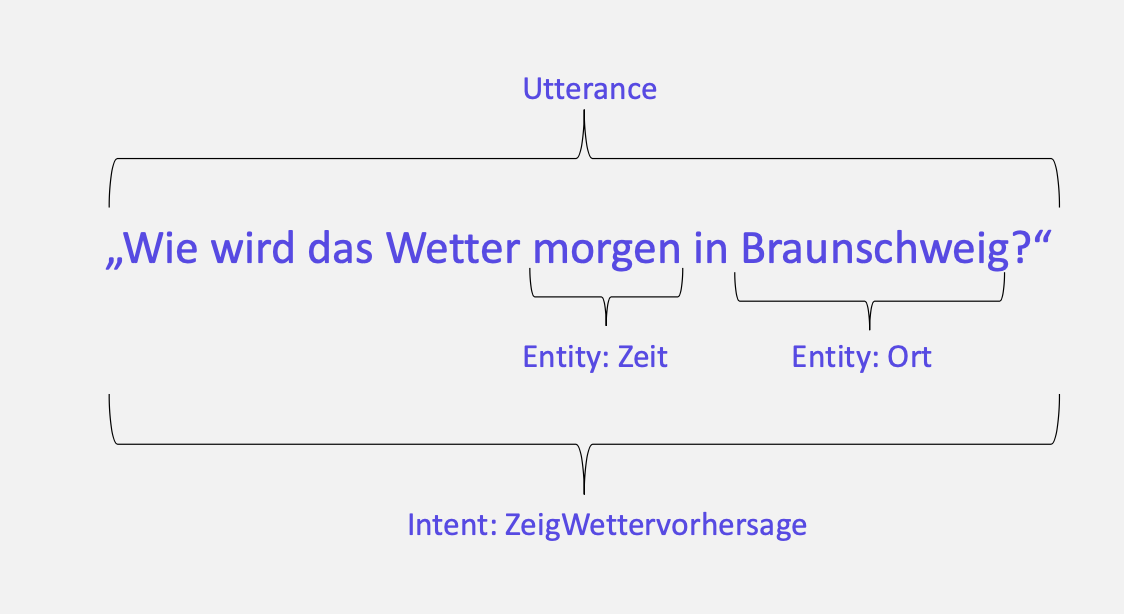
\includegraphics[width=0.6\linewidth]{images/utterance.png}
            \caption[Utterance, Entity, Intent]{Utterance, Entity, Intent (eigene Darstellung, in Anlehnung an \parencite[139]{Sieber.2019})}
            \label{fig:Utterance}
        \end{figure}
        
        Also muss der CA Entities wie \glqq morgen\grqq{}  oder \glqq heute Abend\grqq{} als Vorhersagezeit
        identifizieren, gleiches gilt für den Vorhersageort. 
        Für jeden benutzerdefinierten Intent muss die NLU mit einer Reihe von Anfragen trainiert
        werden, die verschiedene Möglichkeiten darstellen, wie ein Benutzer ein Intent ausdrücken könnte. \parencite[2]{Ahmad.2021}\parencite[138 f.]{Sieber.2019}
        Hier wird deutlich, dass die Formulierungen der Intents von den Benutzern frei gewählt werden können.
        Sobald der CA Pizza als Beispiel für Essen kennt, und der Benutzer nach Kuchen oder Salat fragt, sollte ein gutes NLU-System diese Benutzereingaben
        ebenfalls als Essen kennzeichnen können. \parencite[21]{Kong.2021}
        Dies stellt die Hauptverwendung von ML in Verbindung mit CAs dar, was in Kapitel \ref{ML} näher beschrieben wird.
        Während der Interaktion mit dem Prototypen werden Fragen aus dem ILS-Fragebogen gestellt.
        Der Prototyp muss die Antworten des Lernenden zum jeweiligen richtigen Intent zuordnen und
        Lernverhaltensmerkmale des Lernenden als Entities identifizieren. Diese 
        identifizierten Entities sind für die Lernstilidentifikation
        notwendig, wodurch RQ1 beantwortet werden kann. Der freie Formulierungsgrad spiegelt sich 
        darin wieder, dass die Lernenden auf die Fragen des ILS-Fragebogens unterschiedlich antworten können.

        Wenn eine NLU einen Intent falsch klassifiziert, versteht der CA die Anfrage nicht, was dazu führt, dass der CA auf eine ähnliche
        Anfrage antwortet oder die falsche Aufgabe ausführt.
        Eine falsche Klassifizierung von Entitäten führt hingegen dazu, dass der CA auf eine falsche Information antwortet.
        Um dem entgegenzuwirken, können Fallbacklösungen als Antwort des CAs implementiert werden, um dem Benutzer die Möglichkeit zu geben, 
        seine ursprüngliche Anfrage umzuformulieren. Dabei ist darauf zu achten, wann eine Fallbacklösung ausgelöst werden soll.
        Wird eine Fallbacklösung zu selten ausgeführt und der CA antwortet dadurch häufiger auf unklare Fragen (zu selbstbewusst),
        kann eine zu häufige Ausführung ein unsicheres Verhalten des CAs darstellen, was den Benutzer verärgert, da er die Frage häufig umformulieren muss.
        \parencite[3]{Ahmad.2021}\parencite[139]{Sieber.2019} 
        Aufgrund der geringen Trainingsdaten verwendet der Prototyp die Fallbacklösung.
        
        \subsection{Natural Language Generation}
        NLG wandelt die Antwort des CAs in Text um, der von dem Benutzer gelesen werden kann. 
        Es wird zwischen Template basierter und Deep Learning basierter Methode unterschieden, eine Antwort zu geben.
        Die Template basierte Methode basiert auf vereinfachten und von Menschen erstellten Antworten, welche wenig Flexibilität
        aufzeigen. Dennoch geben diese Antworten eine gute Lesbarkeit für die Menschen. Hingegen kann die Deep Learning basierte Methode flexible
        und personalisierte Antworten erzeugen. Die Antworten werden
        automatisch erstellt. Dadurch ist die Qualität und die Beständigkeit dieser Antworten schwer zu kontrollieren.
        In der Praxis wird oft zu der Template basierten Methode tendiert. 
        Um mehr Flexibilität gewährleisten zu können, wird eine Antwort zufällig aus einem Pool von Template basierten Antworten gewählt. \parencite[24]{Kong.2021}
        Aufgrund von wenigen Trainingsdatensätzen basiert der Prototyp der vorliegenden Arbeit auf einer Template basierten Methode als NLG.
        Die Entwicklung des Deep Learning Ansatzes als NLG kann in der Weiterentwicklung des Prototyps in Betracht gezogen werden. 
       
        \subsection{Dialog Management System} \label{DMS}
        Das DMS ist das Kontrollorgan der Mensch-Maschine Interaktion. Die Hauptaufgabe des DMS besteht darin, den gesamten 
        Unterhaltungsfluss zu koordinieren und zu managen. Durch die Analyse des Kontextes der Unterhaltung entscheidet das DMS, ob die zugrunde 
        liegenden Informationen zur Identifikation der Benutzerabsicht ausreichend sind, um eine entsprechende Aktion oder Datenbankanfrage auszuführen.
        Sobald das DMS nicht genügend Informationen für eine eindeutige Zuordnung der Benutzerabsicht hat, werden die Fallbacklösungen (vgl. Kapitel \ref{NLU})
        eingeleitet. 
        Neben der Steuerung des Ein- und Ausgabeprozesses enthält das DMS den Dialogverlauf. \parencite[23 f.]{Kong.2021} \parencite[59 f.]{Sieber.2019}
        Anhand des Dialogverlaufs können die identifizierten Intents und Entities nachvollzogen werden.
        Während des Dialogs zwischen Prototyp und Lernendem stellt der Prototyp Fragen aus dem ILS-Fragebogen. Die Antworten des Lernenden sollen gesammelt werden, da sie zur Lernstilklassifikation wichtig sind.
        Die 17 Fragen im Dialog werden mithilfe einer Form und Slots ausgeführt. Dies ermöglicht das Sammeln von Informationen des Lernenden. Des Weiteren bietet die Form mithilfe von Slots eine Möglichkeit, dass die einzelnen Fragen in einer gewissen Reihenfolge 
        gestellt werden können. \footnote{\url{ https://rasa.com/docs/rasa/2.x/forms}, aufgerufen am 26.01.2022} Der Slot stellt den Arbeitsspeicher des Bots dar. \footnote{\url{ https://rasa.com/docs/rasa/domain}, aufgerufen am 26.01.2022}  
        Die nächste Frage taucht erst auf, wenn die vorherige Frage beantwortet bzw. der Slot mit seiner zu erwartenden Entity gefüllt wurde.
        Anhand der Antworten des Lernenden zu den Fragen des ILS-Fragebogens können die identifizierten Intents, Entities sowie Slots analysiert werden.
        Mithilfe dieser Analyse kann die Klassifikation des Lernstils geprüft werden.
        
        Das Zusammenspiel der Komponenten NLU, DMS, NLG und Learner stellt das folgende Beispiel dar. Dabei bezieht sich das Beispiel auf eine Frage aus dem ILS-Fragebogen.
        \begin{itemize}
            \item[] \textit{DMS}: Activated Form: ILS-Questionnaire, next question: two
            \item[] \textit{NLG}: Do you tend to be realistic or innovative?
            \item[] \textbf{Learner: I think I tend to be more realistic}
            \item[] \textit{NLU Intent}: ILS-Question-two
            \item[] \textit{NLU Entity}: realistic
            \item[] \textit{DMS}: Activated Form: ILS-Questionnaire, Got Entity, Got Slot with Entity realistic, Slot filled, FS-Dimension-Score: sensor = sensor + 1, next question: three
            \item[] \textit{NLG}: Do you prefer the idea of certainty or hypothesis?
        \end{itemize}

\section{Maschinelles Lernen}\label{ML}
    Die Grundidee des Maschinellen Lernens ist, dass aus Beispielen Regelmä{\ss}igkeiten, Muster oder Modelle extrahiert bzw.
    gelernt werden und mit deren Hilfe neue Daten klassifiziert oder künftige Werte vorhergesagt werden können.
    KI-Systeme, die auf Maschinellem Lernen (ML) beruhen, werden mit diesen Beispielen bzw. Daten (Trainingsinstanzen)
    iterativ trainiert. Die Algorithmen\footnote{ Ein Algorithmus stellt aufeinanderfolgende Anweisungen dar, die ausgeführt werden, damit eine Eingabe in eine Ausgabe transformiert wird. Zum Beispiel kann ein Algorithmus konzipiert werden, der eine unsortierte Menge von Zahlen als Eingabe in eine geordnete Liste ausgibt. \parencite[2]{Alpaydin.2019}}
    des ML lernen aus diesen problemspezifischen Trainingsdaten.
    Sobald die Lernphase beendet ist, entstehen Modelle, welche allgemeine Regeln durch das Erkennen 
    von Mustern, Beziehungen und Regelmäßigkeiten in den Trainingsdaten bilden, um nun korrekte Entscheidungen bei
    unbekannten Daten treffen zu können.
    Der Lernprozess für die Erstellung eines ML-Modells kann in den Lernmodus und Aufgabentyp unterteilt werden. \parencite[35]{deru.2020}
        
        Für das Natural Language Processing werden die Supervised Learning (SL) Ansätze verwendet.
        Das SL Verfahren bildet ein mathematisches Modell ab, welches Datensätze mit Input und 
        dem zu erwartenden Output enthält, sodass dem System vorgegeben wird, was es lernen soll.
        Somit besteht jedes Trainingspaar aus der richtigen Antwort zu jeder Eingabe. Basierend auf diesen 
        Trainingspaaren wird das Modell gelernt, sodass für jede neue Eingabe das System die möglichst  
        korrekte Ausgabe gibt. \parencite[5]{Kong.2021}\parencite[39]{deru.2020}
    
        Der Prototyp dieser Arbeit nutzt unter anderem das SL, um aus unbekannten Benutzereingaben Entities für die Lernstilklassifikation zu extrahieren. 
        Dazu wird er mit einer Reihe von annotierten Texteingaben und 
        Beispielen versehen. Dadurch weiß der Prototyp, wonach er bei unbekannten Benutzeräußerungen 
        suchen soll und wie diese zu interpretieren sind.
           
        CAs beziehen sich auf den Aufgabentyp der Klassifikation.
        Die Aufgabe besteht darin, aus den Merkmalen der eingegebenen Benutzeräußerung
        eine dem Prototypen bekannte Klasse der Intents zu klassifizieren. \parencite[39]{deru.2020} \parencite[37 f.]{gentsch.2018}
        Zum Beispiel 
        soll durch die Benutzereingabe \glqq Hello\grqq{} die Intentklasse \glqq greet\grqq{}
        klassifiziert werden.

        Abschließend unterstützt das ML das NLP, indem die Eingabe des Dialogpartners nicht exakt den, in der Maschine hinterlegten Utterances, 
        entsprechen muss. Denn die Maschine soll die Absicht eines Nutzers ohne zugeordneter Erkennungsregel verstehen und dann antworten. \parencite[142]{Sieber.2019}
        Zum Beispiel soll der Prototyp den Intent \glqq whatDidYouDoYesterday\grqq{} auch bei Utterances wie 
        \glqq I was playing soccer with my friends\grqq{}  oder \glqq I was playing basketball with some students\grqq{} erkennen, sodass 
        unabhängig von der Sportart der Intent klassifiziert wird.
        Dadurch muss nicht jede mögliche Formulierung des Satzes eingegeben werden.
        Grundlage dieses Verhaltens sind Beispieldaten, mit denen die Maschine trainiert wurde. Anhand dieses Lernprozesses lernt 
        die Maschine mithilfe von Wahrscheinlichkeitsvergleichen eigenständig Muster in den Daten zu erkennen und diese der entsprechenden 
        Antwort zuzuordnen.\footnote{\url{ https://www.kiko.bot/blog/allgemein/maschinelles-lernen-bei-chatbots-chatbot-trainieren/}, aufgerufen am 04.01.2022}



    \section{Stand der Forschung} \label{StandderForschung}

    Für die vorliegende Arbeit wurden drei Forschungsarbeiten näher in Betracht gezogen, um RQ1 und RQ2 beantworten zu können.
    Die nachfolgende Abbildung \ref{fig:forschung} skizziert diese.
 
    \begin{figure}[H]
        \centering
        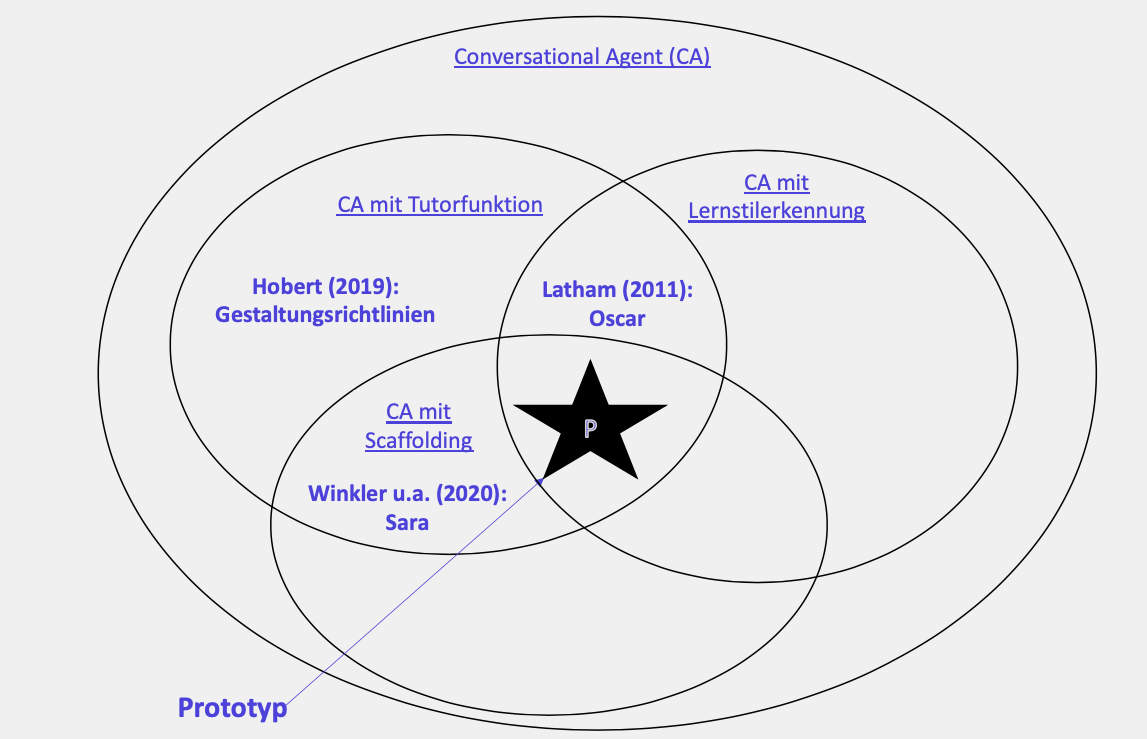
\includegraphics[width=0.9\linewidth]{images/forschung.png}
        \caption[Stand der Forschung]{Stand der Forschung (eigene Darstellung)}
        \label{fig:forschung}
    \end{figure}
    
    In der Literatur kennzeichnet die Hauptaufgabe eines CAs im Education-Bereich die Unterstützung des Lehrbetriebs.
    Hobert (2019) skizziert Gestaltungsrichtlinien zu einem Chatbot basierten Lernsystem, das
    Programmieranfängern beim Lösen von Programmieraufgaben unterstützt, 
    sobald kein menschlicher Lehrassistent verfügbar ist (z.B. am Wochenende).
    Durch diese individuelle Betreuung können Dozenten entlastet werden, sodass
    Programmierkurse auch bei stark steigenden Studierendenzahlen
    durchgeführt werden können. Des Weiteren können die
    meisten Fragen möglicherweise automatisch beantwortet werden, sodass  
    menschliche Lehrassistenten sich auf die Beantwortung der verbleibenden
    schwierigeren Fragen konzentrieren können. \parencite[5 ff.]{Hobert2019SayHT}
    Nach der ersten Designiteration des 
    Coding Tutors wurden Feedbackbögen zu den ersten Skizzen gesammelt.
    Es wurden Studierende in einem Java Anfängerkurs des 
    Studiengangs Wirtschaftsinformatik befragt. Ein auffallender Kommentar war, 
    dass die Befürchtung bestand, dass die \glqq Schritt-für-Schritt-Anleitung\grqq{} den Lerneffekt
    mindern würde, wenn zu viel Anleitung gegeben wird. \parencite[10]{Hobert2019SayHT}
    Der Prototyp der vorliegenden Arbeit gibt beim Quiz-Spiel Hilfestellung zum Lösen der Quiz-Fragen. 
    Dabei wird beachtet, nicht zu viel von der Lösung bei der Hilfestellung zu verraten, sodass 
    der Lernende durch eigene kognitive Anstrengung zur Lösung kommen muss.
        
        Inwiefern CAs den Lehrbetrieb unterstützen können, haben Winkler u.a. (2020) gezeigt und einen CA namens Sara entwickelt, der während einer 
        Online-Vorlesung erscheint. 
        Sara unterbricht den Videovortrag nach jedem Unterkapitel
        und stellt jedem Lernenden eine Reihe von Verständnisfragen, um den gerade gesehenen und gehörten Inhalt zu wiederholen.
        Dabei können die Lernenden mit Sara per Text oder Stimme interagieren.
        Bei einer richtigen Antwort fährt Sara mit der nächsten Frage fort. 
        Wenn Sara eine falsche Antwort erkennt, oder der Lernende nicht weiß,
        wie er antworten soll, öffnet sich ein weiteres Dialogfenster für Erklärungen und Fragen 
        des Lernenden. Nach der Erklärung wird die Frage erneut gestellt, und die Lernenden haben noch einmal die Möglichkeit, 
        die Frage erneut zu beantworten, bevor die Antwort erklärt wird und Sara mit der nächsten Frage fortfährt. \parencite[4 f.]{winkler_hobert_salovaara_söllner_leimeister_2020}
        Mit diesem Mechanismus versucht Sara, das scaffolding Verhalten von Pädagogen in der Interaktion mit ihren Lernenden zu imitieren. 
        Das scaffolding Verhalten von Pädagogen bezeichnet eine Unterstützung des Lernprozesses durch die Bereitstellung einer ersten Orientierungsgrundlage
        in From von Anleitungen oder Denkanstößen. \footnote{\url{https://lexikon.stangl.eu/13399/scaffolding}, aufgerufen am 18.11.2021}
        Der Prototyp dieser Arbeit greift beim Quiz-Spiel auf das Scaffolding Verhalten zurück. Bei einigen 
        Quiz-Fragen werden dem Lernendem  
        Hilfsfragen gegeben, um auf die richtige Lösung zu kommen.
        Die Ergebnisse der Studie zeigen einen positiven Effekt auf die Verwendung eines scaffolding textbasierten CA.
        Lernende, welche mit einem scaffolding textbasierten CA im Lernprozess interagiert haben, haben im Vortest zu der Programmiersprache Python ohne 
        einen scaffolding CA
        39.8 Punkte von 100 Punkten und im Nachtest mit einem scaffolding CA 73,1 Punkte von 100 Punkten erreicht. \parencite[8 f.]{winkler_hobert_salovaara_söllner_leimeister_2020}

        Latham u.a. (2010) haben ein conversational intelligent tutoring system (CITS)  namens Oscar entwickelt, der während eines Nachhilfegesprächs den Lernstil des Lernenden bestimmt und dann sein Lehrformat
        an den identifizierten Lernstil des Lernenden anpasst.
        Ein  intelligentes conversational Tutoringsystem sind Computerlernsysteme, die ihre Lerninhalte für eine Person personalisieren und über eine 
        natürliche Sprachschnittstelle zur Kommunikation per Text oder Sprache verfügen.
        Oscar klassifiziert den Lernstil nach dem Lernstilmodell 
        von Felder und Silverman (1988). Dafür nutzt Oscar den ILS-Fragebogen von Felder und Soloman (1991) (vgl. Kapitel \ref{ATL}).
        Oscar zielt darauf ab, einen menschlichen Tutor nachzuahmen, 
        indem er eine dialogorientierte Problemlösungsunterstützung im Bereich der 
        Datenbank Structured Query Language (SQL) anbietet.
        Zur Unterstützung des Nachhilfegesprächs können Diagramme, Bilder und interaktive Filme angezeigt werden. Aspekte des Verhaltens 
        und des Verständnisses des Lernenden fließen in die dynamische Einschätzung
        des Lernstils ein und ermöglichen es, den Unterrichtsstil so zu personalisieren, dass er am besten zu dem Schüler passt.
        \parencite[4]{Oscar}

        Der ILS-Fragebogen enthält 44 Fragen. Es wurde eine Pilotstudie mit 103 ausgefüllten ILS-Fragebögen durchgeführt,
        um zu untersuchen, welche Fragen die aussagekräftigsten waren, um den Lernstil zu bestimmen. 
        Die Studie ergab, dass 17 Fragen den gesamten Lernstil zu mindestens 75 \% vorhersagen können. 
        Sobald eine begrenzte Anzahl von ILS-Fragen in einen CITS zur Vorhersage des individuellen Lernstils des Lernenden 
        einbezogen werden, ist es am besten, diejenigen Fragen auszuwählen, die den allgemeinen Lernstil am genauesten vorhersagen.
        Für die Beurteilung des allgemeinen Lernstils als auch für dessen Stärke werden alle Fragen des ILS-Instruments benötigt.
        Allerdings sobald das Ausfüllen des ILS-Fragebogens
        durch eine implizite Vorhersage des Lernstils ersetzt wird, so ergibt sich aus den Studienergebnissen ein Ausgangspunkt für die Fragen, die am besten 
        den allgemeinen Lernstil bestimmen können. \parencite[51 f.]{Latham.2011}
        
        Das FS-Modell wurde für die Klassifizierung des Lernstils von Ingenieurstudenten entwickelt.
        In einer weiteren Pilotstudie mit 10 Teilnehmern wurde Oscar auf zwei Arten beurteilt.
        Sowohl wurde die Einschätzung des Lernstils durch Oscar bewertet als auch die Art und Weise, wie Oscar von dem Benutzer 
        während der Interaktion wahrgenommen wurde.
        Während des Tutor-Gesprächs werden die Lernstilwerte in Abhängigkeit vom Gespräch des Lernenden erhöht.
        Am Ende der Tutoring-Sitzung werden die Wertepaare jeder FS-Dimension verglichen, um die allgemeine Lernstiltendenz 
        des Schülers für diese Dimension (d.h. der höhere Wert) anzuzeigen. Die Werte des Lernstils hängen von der individuellen
        Tutorial-Sitzung einer Person ab. Sobald eine Kategorie nicht eindeutig bestimmt werden konnte, die einer bestimmten FS-Dimension nahelag,
        bleibt dieser Lernstil unklassifiziert. 
        Bei der Studie wurden drei Experimente durchgeführt.
        Experiment eins untersuchte die Art und Weise, wie der Lernende mit dem Lernmaterial und mit der Hilfestellungen von Oscar umging.  
        Experiment zwei untersuchte die Anzahl der Interaktionen mit Oscar während des Tutorials.
        Für das zweite Experiment wurde die Anzahl der Interaktionen während der Tutoring-Sitzung gezählt. 
        Die Hypothese lautete: \glqq Je diskursiver ein Schüler 
        ist (d. h. je mehr Interaktionen), desto mehr neigen sie zum verbalen Lernstil\grqq{}.
        Für Experiment drei wurde die 
        durchschnittliche Zeit zum Lesen von zehn Oscar-Wörtern für jeden Schüler berechnet.
        Die Hypothese war, dass \glqq je länger ein Schüler braucht, um Anweisungen zu lesen 
        (d. h. je weniger er mit Wörtern vertraut ist), desto mehr tendieren sie zum visuellen Lernstil\grqq{}. 
        Für die Studie wurden Studierende der Ingenieurswissenschaft ausgewählt, welche einen Pre-Test im Bereich SQL absolviert haben sowie den ILS-Fragebogen ausgefüllt haben.
        Nach dem Gespräch mit Oscar haben die Lernenden einen Post-Test durchgeführt. Der identifizierte Lernstil von Oscar 
        wurde mit dem Lernstil aus dem Fragebogen verglichen.
        Die Ergebnisse der ersten Pilotstudie sind vielversprechend, da in drei Fällen die Genauigkeit der Schätzung des Lernstils bei 70 \% lag und im schlechtesten Fall bei 50 \%.
        Darüber hinaus haben sich die 
        Testergebnisse zwischen Pre- und Post-Test um ca. 21 \% verbessert. Dennoch kann mit dieser kleinen Ausgangsstichprobe keine 
        eindeutige Schlussfolgerungen gezogen werden, daher bedarf es an einer weiteren Studie mit einer größeren Stichprobengruppe. \parencite[6 f.]{Oscar}

        Eine weitere Studie zu Oscar wurde mit 65 Lernenden durchgeführt, die bereits Erfahrung mit einem Bachelor-SQL-Kurs hatten. 
        Dabei wurden zu den drei bestehenden Experimenten noch zwei weitere hinzugefügt. Ferner wurde zusätzlich noch der Stil der 
        Tutorialfragen untersucht, bei denen die Teilnehmer die richtige Antwort gaben.
        Es wurde die Anzahl der richtigen theoretischen und der richtigen praktischen Fragen gezählt.
        Oscar hat den Lernstil als aktiv und sensorisch bei den Lernenden eingestuft, die in theoretischen Fragen bessere Leistungen zeigten. Bei 
        schlechterer Leistung in theoretischen Fragen
        wurden die Lernenden als reflektierend und intuitiv klassifiziert.
        Des Weiteren wurde eine Tutorial-Frage als eine allgemeine \glqq Trick-Frage\grqq{} gestellt, bei
        der die Antwort im erläuternden Text stand. Dadurch wurde die Detailgenauigkeit und Lesefähigkeit des Lernenden getestet. 
        Lernende, welche die Frage nicht richtig beantworteten, wurden als visuelle und intuitive Lerner bestimmt, während diejenigen,
        die richtig antworteten, als verbale und sensorische Lerner eingestuft wurden.
        Die experimentellen Ergebnisse zeigen, dass es möglich ist, einen Lernstil aus einem wechselseitigen Nachhilfegespräch
        in natürlicher Sprache vorherzusagen. Oscar hat alle Lernstile mit einer Genauigkeit zwischen 61-100 \% 
        im Rahmen des Index of Learning Styles erfolgreich klassifiziert.  \parencite[105 ff.]{Latham.2012}
        
        Der Prototyp dieser Arbeit verwendet in seinem Dialog zur Lernstilidentifikation des Lernenden 
        die 17 reduzierten Fragen des ILS-Fragebogens von Latham (2011). Allerdings findet die Klassifikation 
        des Lernstils, nicht während eines Nachhilfegesprächs statt, sondern in einem freundlichen Dialog.
        Dem Lernenden wird der identifizierte Lernstil am Ende des Dialogs mitgeteilt, sodass er sein 
        Lernverhalten diesem anpassen kann. Des Weiteren wendet sich der Prototyp im Gegensatz zu Oscar an allgemein Lernende, unabhängig vom 
        Studiengang. Zusätzlich bestimmt der Prototyp den Lernstil ein weiteres Mal in einer zweiten Interaktion zwischen 
        Lernendem und Prototypen. In einem Quiz-Spiel wird durch die angebotenen Hilfestellungen versucht, den Lernstil 
        des Lernenden zu identifizieren. Dabei wird sich an die Vorgehensweise von Oscars Hilfestellungen und Quiz-Fragen (Experiment 1, 4 und 5) während 
        seines Nachhilfegesprächs zu SQL orientiert. 

        An dieser Stelle soll noch einmal zu der aufgeführten Abbildung \ref{fig:forschung} Bezug genommen werden.
        Der Prototyp adaptiert von allen drei vorgestellten Forschungsansätzen einige Aspekte. Deshalb 
        findet er in der Abbildung dort seinen Platz, wo sich alle Kreise überschneiden. 

    \textbf{Kapitelzusammenfassung} 
    \begin{itemize}
        \item Conversational Agents können auf text- oder sprachbasierter natürlicher Sprache mit dem Benutzer interagieren. Dabei werden textbasierte Conversational Agents oft als Chatbots bezeichnet, mit denen über Textnachrichten interagiert wird. Für die Beantwortung von RQ1 und RQ2 führt der Lernende zwei textbasierte Interaktion mit dem Prototypen durch.
        \item Ein Virtual Companion dient als vertrauenswürdiger Begleiter des Benutzers.
        \item Der Einstieg ins NLP und ML wurde gegeben, um ein Verständnis für die Computerlinguistik zwischen Mensch und Maschine zu bekommen.
        \item NLP bietet eine Möglichkeit für Computer, die menschliche Sprache auf intelligente und nützliche Weise zu analysieren, zu verstehen und Bedeutungen abzuleiten.
        NLP setzt sich aus NLU und NLG zusammen.
        \item Das Hauptziel von NLU besteht darin: beim Prozess der autonomen Gesprächsführung, strukturierte Daten aus unstrukturierten Spracheingaben des Benutzers zu extrahieren.
        Somit extrahiert die NLU Intents und Entities aus Benutzeranfragen.
        Dabei stellen Intents die Benutzerabsicht, Entities die wichtigen Informationen aus der Anfrage und die Utterances die unterschiedlichen Benutzeräußerungen dar.
        \item Der Prototyp muss die Antworten des Lernenden zum richtigen Intent zuordnen und Lernverhaltensmerkmale des Lernenden als Entities identifizieren. Diese identifizierten Entities sind für die Lernstilidentifikation notwendig, wodurch RQ1 beantwortet werden kann.
        \item NLG wandelt die Antwort des CAs in Text um, der von dem Benutzer gelesen werden kann.
        \item Das DMS ist das Kontrollorgan der Mensch-Maschine Interaktion. Die Hauptaufgabe des DMS besteht darin, den gesamten Unterhaltungsfluss zu koordinieren und zu managen. Die 17 Fragen des ILS-Fragebogens werden im Dialog  mithilfe einer Form und Slots ausgeführt. Dies ermöglicht das Sammeln von Lernstilmerkmalen des Lernenden, wodurch die Lernstilklassifikation möglich wird. 
        \item Das ML unterstützt das NLP, indem die Eingabe des Dialogpartners nicht exakt den, in der Maschine hinterlegten Utterances, entsprechen muss. Die Maschine soll die Absicht eines Nutzers ohne zugeordneter Erkennungsregel verstehen und antworten können. Dadurch können die Lernenden auf die Fragen des ILS-Fragebogens unterschiedlich antworten. Des Weiteren wird das Extrahieren von Entities für die Lernstilklassifikation ermöglicht.
        \item Ein Bezug zu anderen Arbeiten sowie deren Abgrenzung wurde mithilfe des aktuellen Forschungsstandes aufgezeigt.
        Die gewonnenen Erkenntnisse, wie zum Beispiel das Scaffolding-Verhalten und die 17 reduzierten ILS-Fragen,
        wurden bei der Implementierung des Prototyps berücksichtigt, welche 
        im nachfolgenden Kapitel bei der Vorstellung des Prototyps näher aufgezeigt werden. 
    \end{itemize}
\chapter{Prototyp eines Conversational Agents zur Identifikation von Lernstilen}
\chaptermark{Prototyp}
Im Folgenden wird eine kurze Erläuterung zu dem Framework gegeben, das der Prototyp dieser Arbeit nutzt (Kapitel \ref{RasaFramework}),
um den groben Funktionsaufbau des Prototyps zu verstehen.
Anschließend wird der Prototyp vorgestellt (Kapitel \ref{VorstellungPrototyp}). Der Lernende durchläuft zwei Interaktionen mit 
dem Prototypen. Zuerst führt der Prototyp mit dem Lernenden ein Dialog. Aufgrund der Antworten des 
Lernenden klassifiziert der Prototyp dessen Lernstil. 
Anschließend führt der Prototyp mit dem Lernenden 
ein Quiz-Spiel durch, bei dem der Lernende aus vier oder acht Quiz-Fragen wählen kann. 
Hierbei wird der Lernstil des Lernenden zu einem weiteren Mal bestimmt. \footnote{Für den weiteren Verlauf der Arbeit gilt, dass die erste Interaktion mit dem Prototypen den Dialog repräsentiert. Zur abwechslungsreicheren Gestaltung wird als Synonym dafür das Wort Gespräch verwendet. Die zweite Interaktion stellt das Quiz-Spiel dar. } 
Die Lernstilklassifikation ist für die Beantwortung von RQ1 relevant.
Das Kapitel \ref{VorstellungPrototyp} unterteilt sich aufgrund der zwei unterschiedlichen Interaktionen 
in zwei Teilkapitel, in denen jeweils eine ausführlichere Erläuterung zur jeweiligen Interaktion gegeben wird.
Außerdem endet jedes Teilkapitel mit visuellen Gesprächsauszügen aus der jeweiligen Interaktion.


\section{Framework Rasa}\label{RasaFramework}
Rasa ist ein Open Source Machine Learning Framework, mit dem CAs und intelligente Systeme gebaut werden können. 
Rasas modulares und flexibles Design bietet Entwicklern leicht die Möglichkeit neue Erweiterungen und Funktionalitäten zu implementieren.
Das Framework unterteilt sich in vier Hauptbestandteile: \textbf{NLU}, \textbf{Core}, \textbf{Channel} und \textbf{Hilfsfunktionen}.
Das \textbf{NLU} befasst sich mit Intents und der Extraktion der Schlüsselinformationen (Entities).
Der \textbf{Core} ist verantwortlich dafür, dass der CA die bestmögliche Antwort zurückgibt sowie die nächste auszuführende Aktion bezüglich des Dialogs bestimmt.
Der \textbf{Channel} stellt die Verbindung zwischen CA und Nutzer dar.
\textbf{Hilfsfunktionen} können beispielsweise als Zugang zum gespeicherten Gesprächskontext dienen. \parencite[25]{Kong.2021} 

Es gibt viele Möglichkeiten einen CA zu bauen. Diese Möglichkeiten lassen sich in Closed-Source-Lösungen und in Open-Source-Lösungen unterteilen.
Closed-Source-Lösungen haben Nachteile wie, z.B. hohe Kosten, eine Bindung an einen bestimmten Anbieter, das Risiko von Datenverlusten und die Schwierigkeit
benutzerdefinierte Funktionen zu implementieren. Bei Open-Source-Lösungen gibt es diese Probleme nicht. Ein Nachteil von Open-Source-Lösungen ist,
dass die Benutzer ein gutes CA-Framework sorgfältig auswählen müssen, welches über eine große Skalierbarkeit und leistungsstarke Funktionen verfügt. Des Weiteren sollte es
einfach zu erlernen sein und eine aktive Community haben. Rasa verfügt über all diese Eigenschaften. \parencite[25]{Kong.2021}

\textbf{System Architektur}

Die System Architektur besteht aus den zwei Hauptteilen Rasa und dem Rasa Software Development Kit (Rasa SDK).
Rasa enthält die oben beschriebenen NLU und Core. 
Rasa NLU wandelt die Eingaben des Benutzers in Intents und Entities (vgl. Kapitel \ref{NLP}) um. 
Rasa Core entscheidet über die nächste Aktion auf der Grundlage von aktuellen und historischen Dialogaufzeichnungen.
Solche Aktionen können die Beantwortung einer bestimmten Nachricht eines Benutzers sein oder der Aufruf einer Aktionsklasse,
die auf den Benutzer zugeschnitten ist. \parencite[26]{Kong.2021} Der Arbeitsprozess von Rasa ist in der Abbildung \ref{fig:Rasa} abgebildet.
\begin{figure}[H]
  \centering
  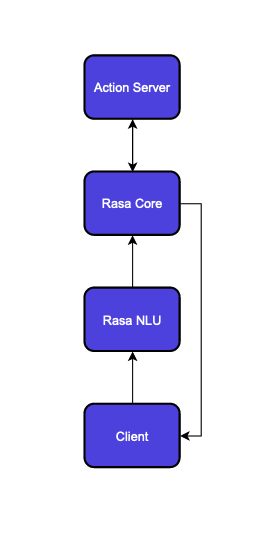
\includegraphics[width=0.25\linewidth]{images/rasa.png}
  \caption[Arbeitsprozess von Rasa]{Arbeitsprozess von Rasa (eigene Darstellung, in Anlehnung an \parencite[26]{Kong.2021})}
  \label{fig:Rasa}
\end{figure} 
Rasa bietet das Rasa SDK an, um Entwicklern bei der Erstellung ihrer benutzerdefinierten Aktionen zu helfen.
Der Prototyp dieser Arbeit benutzt benutzerdefinierte Aktionen unter anderem für die Klassifikation des Lernstils des Benutzers, 
die Erläuterung des klassifizierten Lernstils, die Logik des Quiz-Spiels, die Handhabung von Chitchat und Killerphrasen sowie weiteren kleinen Hilfsfunktionen wie 
z.B. der Namensidentifizierung.
Eine benutzerdefinierte Aktion wird in einem eigenen Server ausgeführt und wird daher auch als Action Server bezeichnet.
Der Action Server kommuniziert mit Rasa Core über das Hyper Text Transfer Protocol (HTTP). \parencite[26]{Kong.2021}

Rasa Core und Rasa NLU arbeiten eng miteinander und sind in einem Package organisiert verbunden.
Rasa SDK liegt in einem anderen individuellen Software Package.
Der Grund für diese Unterteilung ist, dass Rasa NLU und Rasa Core von einem Algorithmen Team entwickelt werden,
während die benutzerdefinierten Aktionen von dem Python
Programmierungs Team entwickeln werden. \parencite[27]{Kong.2021}

\textbf{Pipeline}

Eine Pipeline in Rasa definiert die Abhängigkeitsbeziehung und die Richtung des Datenflusses zwischen den verschiedenen Komponenten.
Die unterschiedlichen Komponenten unterteilen sich in: 
\textbf{Tokenizer}, \textbf{Featurizer}, \textbf{Entity extractor} und \textbf{Intent classifier}.
Der \textbf{Tokenizer} zerlegt den Text in kleine Textabschnitte, welche als Tokens bezeichnet werden.
Der \textbf{Featurizer} ist dafür verantwortlich, dass Merkmale aus Token-Sequenzen extrahiert werden.
Der \textbf{Entity extractor} führt eine Entity Extraktion auf dem Text durch und verwendet dabei
 die von den vorherigen Komponenten bereitgestellten Merkmalen.
Der \textbf{Intent classifier} sorgt dafür, dass der Text je nach Kontext in verschiedene Benutzerabsichten unterteilt wird. \parencite[39]{Kong.2021} 

Als Tokenizer nutzt der Prototyp, welcher die englische Sprache verwendet, den WhitespaceTokenizer. Dieser erzeugt ein Token für jede durch ein Leerzeichen getrennte Zeichenfolge. \footnote{\url{https://rasa.com/docs/rasa/components}, aufgerufen am 19.12.2021}
Zudem wird dieser Tokenizer bei der Verwendung der englischen Sprache empfohlen. \parencite[40]{Kong.2021}\\
Als Featurizer Komponente wurde der Regex Featurizer genutzt. Während des Trainings erstellt dieser eine Liste von regulären Ausdrücken,
die im Trainingsdatenformat definiert sind. Für jedes Regex wird ein Merkmal gesetzt, das angibt, ob dieser Ausdruck in der Benutzernachricht
gefunden wurde oder nicht. \footnote{\url{https://rasa.com/docs/rasa/components}, aufgerufen am 20.12.2021}
Beim Prototypen wurden Antworten als Regex hinterlegt, um mathematische Antworten beim Quiz-Spiel, welches die zweite Interaktion
zwischen Lernendem und Prototypen darstellt, zu erkennen und zu validieren.
Als eine weitere Featurizer Komponente wurde der Count Vector genutzt, um Rechtschreibfehler des Benutzers abzufangen.
Des Weiteren wurde auf den Lexical Syntatic Featurizer zurückgegriffen, dadurch werden lexikalische und syntaktische Merkmale
für eine Benutzernachricht zur Unterstützung der Entity Extraktion erstellt. Zum Beispiel wird ein Merkmal erstellt, um zu erkennen, ob der Anfangsbuchstabe des Wortes 
groß oder klein geschrieben ist. \footnote{\url{https://rasa.com/docs/rasa/components}, aufgerufen am 20.12.2021}\\
Als Entity extractor und Intent classifier wird DIET (Dual Intent and Entity Transformer) genutzt. Dies ist eine Multi-Task-Architektur zur Klassifizierung von Intents
und zur Erkennung von Entities. So kann aus der Utterance \glqq I want to play soccer\grqq{} der Intent \textit{PlayGame} klassifiziert werden und
die Entity \textit{Game:} \glqq soccer\grqq{} extrahiert werden. Auf den basierenden Erfahrungen von Kong und Wang, wird die Verwendung von 
DIET aus Performancegründen empfohlen. \parencite[47]{Kong.2021}
Außerdem wurde ein Fallback classifier genutzt, um Nutzernachrichten abzufangen, die einem Intent nicht eindeutig zuzuordnen sind. 
Ebenfalls bietet der verwendete Entity Synonym Mapper die Möglichkeit Synonyme für einzelne Entitäten in den Trainingsdaten zu verwenden. \footnote{\url{https://rasa.com/docs/rasa/components}, aufgerufen am 20.12.2021}
Zum Beispiel kann der Lernende bei der Frage des Prototyps: \glqq Do you prefer the idea of certainty or theory?\grqq{}  
Anstatt \glqq I prefer the idea of certainty.\grqq{} mit \glqq I prefer the idea of truth.\grqq{} antworten. Somit stellt \textit{truth} ein Synonym für \textit{certainty} dar.


\section{Vorstellung des Prototyps}  \label{VorstellungPrototyp}

Der Prototyp \footnote{Der Source-Code ist auf dem beigelegten USB-Stick zu finden. Eine Anleitung zum Aufruf befindet sich im  Anhang \ref{Source-Code}.} hat zwei implementierte Interaktionen. Zuerst durchlebt der Lernende ein Dialog mit dem Prototypen.
Der Dialog wird aktiv von dem Prototypen geführt. Während des Dialogs werden 17 Fragen des ILS-Fragebogen gestellt, und 
anhand der Antworten des Benutzers wird der Lernstil klassifiziert. 
Anschließend kann der Lernende zwischen einem vier oder acht Fragen Quiz-Spiel wählen. Nach der zweiten Interaktion
bestimmt der Prototyp den Lernstil des Benutzers erneut.

\subsection{Interaktion: Dialog}
Das Problem bei Fragebögen besteht darin,
dass das Ausfüllen für die Lernenden zeitaufwändig und mühsam ist.
Aufgrund dessen füllen sie diese nicht genau aus,
was zu einer falschen Bewertung 
des Lernstils führt \parencite[189 f.]{Popescu.2009}
Der ILS ist ein Fragebogen zur Selbsteinschätzung (vgl. Anhang \ref{44ILS}), 
der 44 Fragen enthält, wobei sich jeweils elf Fragen auf eine der vier FS-Dimensionen beziehen.
Für jede Frage gibt es zwei mögliche Antworten a und b. Treffen beide Antwortmöglichkeiten
auf den Lernenden zu, muss er eine der Antworten wählen, die auf ihn am meisten zutrifft. \footnote{\url{https://www.webtools.ncsu.edu/learningstyles/}, aufgerufen am 23.12.2021} 
Nachdem alle Fragen beantwortet wurden, wird die Gesamtzahl der a- und b-Antworten
für jede FS-Dimension verglichen, und die höhere Summe repräsentiert den Lernstil.
Für die Dimension aktiv/reflektierend ist der Gesamtlernstil beispielsweise 
reflektierend, wenn die Gesamtsumme des Fragebogens a = 3 und b = 8 ist,
da die Gesamtzahl der b-Antworten höher ist.  

Wenn Bewertungsfragen aus dem ILS-Fragebogen in ein CA-Gespräch integriert werden sollen,
muss die Anzahl der Fragen reduziert werden. \parencite[49 f.]{Latham.2011}
Daher hat Latham (2011) eine Studie zur Reduktion der Fragen des Fragebogens durchgeführt.
Die Ergebnisse zeigen, dass einige Fragen den Lernstil
genauer vorhersagen als andere, sodass die Anzahl der Fragen reduziert werden kann.
17 der 44 Fragen wurden mit einer Genauigkeit von 75 Prozent oder besser bei der Vorhersage des gesamten Lernstils identifiziert. \parencite[62]{Latham.2011}
Es werden sowohl sechs von den 17 Fragen der FS-Dimension 
visuell/aktiv zugeordnet als auch sechs zu der FS-Dimension sensorisch/intuitiv. 
Zu der FS-Dimension aktiv/reflektiv gehören zwei von den ausgewählten 17 Fragen.
Die verbleibenden drei Fragen werden der FS-Dimension 
sequentiell/global zugeordnet.
Um den Gesprächsfluss zu strukturieren, wurden die 17 ausgewählten Fragen des ILS-Fragebogens
in drei Themenbereiche eingeteilt. 
Die Tabelle ist im Anhang \ref{17-ILS-Fragebogen} vorzufinden.
Die Fragen Q1-Q3 werden der Kategorie \textbf{Smalltalk} zugeordnet. Der Dialog zur Lernstilklassifikation  
startet nach der Begrüßung mit einer offenen Frage \glqq What did you do yesterday in the evening?\grqq{}
und stellt den Übergang zur Frage Q1 dar.\\ 
Die Fragen Q4-Q6 repräsentieren die Kategorie \textbf{Persönlichkeit}. Nachdem die erste Kategorie abgeschlossen wurde, 
wird der Prototyp im Dialog konkret, indem der Prototyp die Fragen der zweiten Kategorie durch 
\glqq I´m interested in your personality.\grqq{} einläutet.\\
Die dritte Kategorie \textbf{Studienleben} wird durch die Fragen Q7-Q17 dargestellt.
Mit dem Ausdruck \glqq Let´s talk about your study life.\grqq{} wird dem Lernenden der Wechsel des Themas
mitgeteilt. Für die Storyline des Dialogs mussten die originalen ILS-Fragen leicht abgeändert werden.
Dies war nötig, um erstens eine flüssige Storyline zu erstellen und zweitens die Gefahr bestand, bei einigen originalen ILS-Fragen gleich zu antworten. 
Zum Beispiel bei der Frage mit dem Index Q1 und bei der Frage mit dem Index Q14 kann in beiden Fällen mit \glqq picture\grqq{} geantwortet 
werden (vgl. Anhang \ref{17-ILS-Fragebogen}). Die NLP-Komponente von Rasa bekommt Schwierigkeiten bei der Klassifizierung des richtigen Intents,
sobald auf unterschiedliche Intents die gleiche 
Antwort gegeben werden kann. Deshalb mussten die Fragen so angepasst werden, dass auf jede Frage 
unterschiedlich geantwortet werden kann.  


Mit der Hilfe der Wizard of Oz (WoZ) Methode wurde
eine erste erstellte Storyline getestet und angepasst. Bei der WoZ Methode interagieren Testpersonen 
mit einem autonomen System, bei dem jedoch ein menschlicher Akteur die Befehle ausführt 
und sich dabei so verhält, als wäre er die Software. \parencite[27]{Kelley.1984}
Das Ziel war es dabei, die Struktur und das Verständnis der gestellten Fragen zu prüfen und anschließend anzupassen.
Des Weiteren diente es zur Aufnahme von Trainingsdaten, um mögliche Eingaben des Benutzers auf die gestellten Fragen des Prototyps zu sammeln.
Das dokumentierte Gespräch befindet sich im Anhang \ref{tab:/Anhang_Dialogflow/G}.

Wie auch beim Ausfüllen des ILS-Fragebogens (siehe oberer Abschnitt) darf der Lernende für jede Frage nur eine Antwort wählen und muss alle Fragen beantworten. Wenn sowohl 
die eine Antwortmöglichkeit als auch die andere auf den Lernenden zu trifft, sollte er diejenige wählen, 
die auf ihn häufiger zutrifft. \footnote{\url{https://www.webtools.ncsu.edu/learningstyles/}, aufgerufen am 23.12.2021} 
In Abhängigkeit von der gewählten Antwort erhöht sich die Tendenz des Lernenden zu einem Lernstil, welcher die Antwortmöglichkeit 
gerade repräsentiert, dies merkt sich der Prototyp.



\textbf{Vorstellung Dialog} 

Die nachfolgende Abbildung enthält einen beispielhaften Gesprächsverlauf zwischen einem 
Lernenden und dem Prototypen namens Vicky. Die rote Markierung stellt den Bezug von Vickys gestellter Frage zur der
ausgehenden ILS-Frage (vgl. Anhang \ref{17-ILS-Fragebogen}).
\begin{figure}[H]
  \centering
  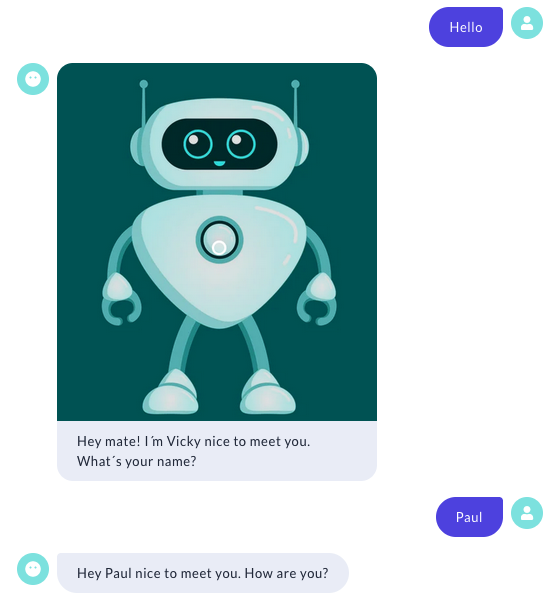
\includegraphics[width=0.7\linewidth]{images/Talk_roterMarker/T0.PNG}
  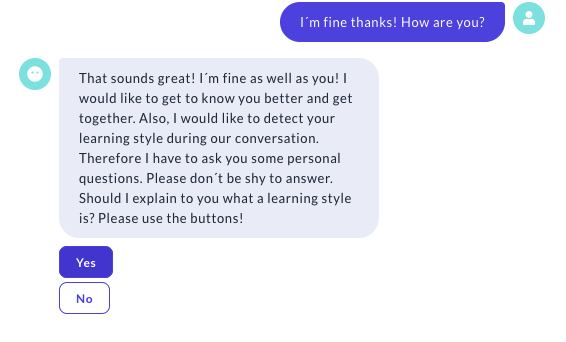
\includegraphics[width=0.7\linewidth]{images/Talk_roterMarker/T0.2.png}
 \end{figure} 
  \begin{figure}[H]
    \centering
    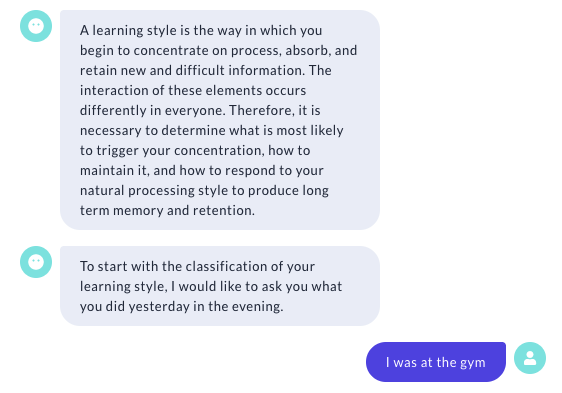
\includegraphics[width=0.7\linewidth]{images/Talk_roterMarker/T0.3.PNG}
    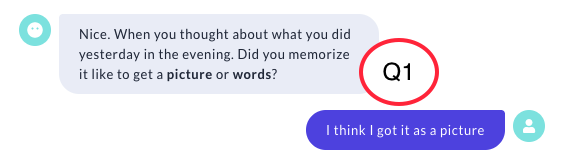
\includegraphics[width=0.7\linewidth]{images/Talk_roterMarker/T1.PNG}
    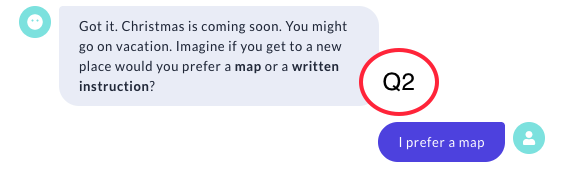
\includegraphics[width=0.7\linewidth]{images/Talk_roterMarker/T2.png}
    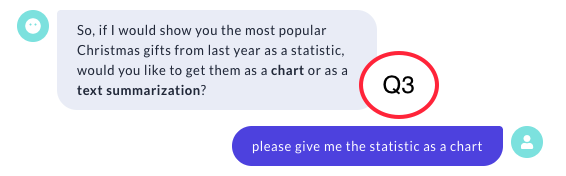
\includegraphics[width=0.7\linewidth]{images/Talk_roterMarker/T3.png}
    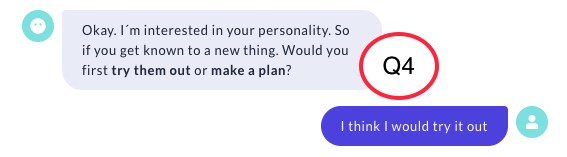
\includegraphics[width=0.7\linewidth]{images/Talk_roterMarker/T4.png}
    \label{fig:GesprächI}
\end{figure} 
\begin{figure}[H]
  \centering
  
\includegraphics[width=0.7\linewidth]{images/Talk_roterMarker/T5.png}
  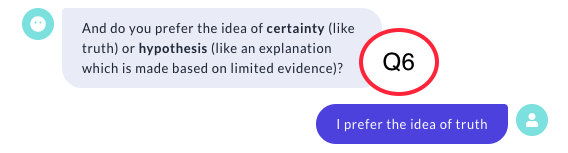
\includegraphics[width=0.7\linewidth]{images/Talk_roterMarker/T6.png}
  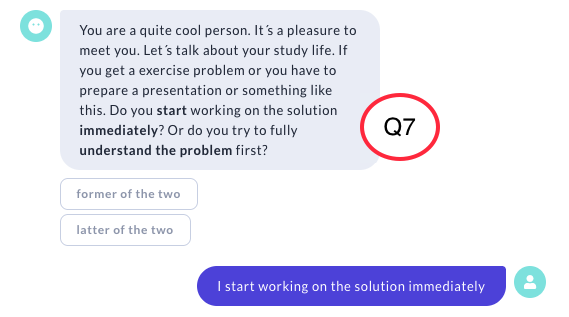
\includegraphics[width=0.7\linewidth]{images/Talk_roterMarker/T7.png}
  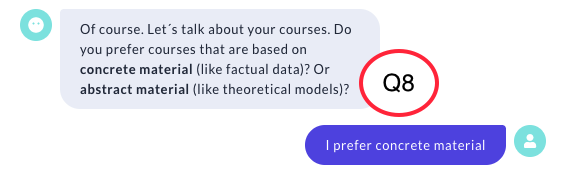
\includegraphics[width=0.7\linewidth]{images/Talk_roterMarker/T8.png}
  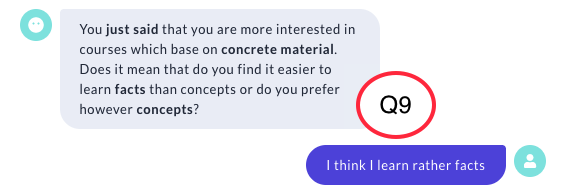
\includegraphics[width=0.7\linewidth]{images/Talk_roterMarker/T9.png}
  \label{fig:GesprächII}
\end{figure} 
\begin{figure}[H]
  \centering
  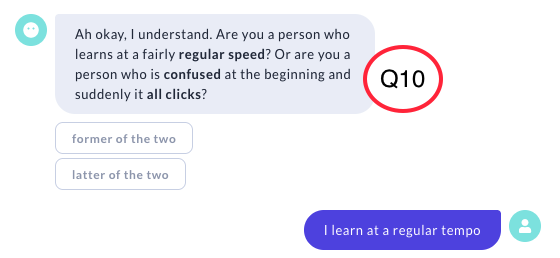
\includegraphics[width=0.7\linewidth]{images/Talk_roterMarker/T10.png}
  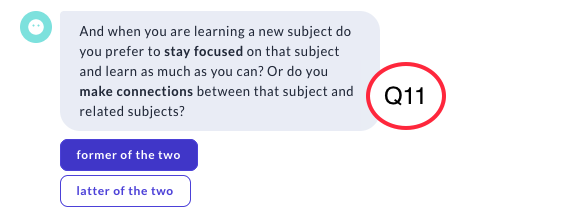
\includegraphics[width=0.7\linewidth]{images/Talk_roterMarker/T11.png}
  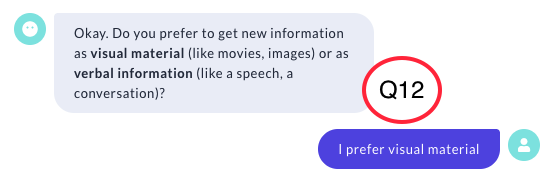
\includegraphics[width=0.7\linewidth]{images/Talk_roterMarker/T12.png}
  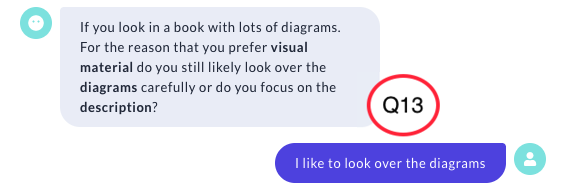
\includegraphics[width=0.7\linewidth]{images/Talk_roterMarker/T13.png}
  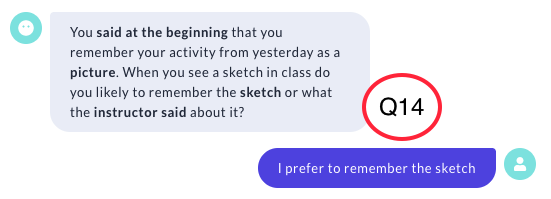
\includegraphics[width=0.7\linewidth]{images/Talk_roterMarker/T14.png}
  \label{fig:GesprächIII}
\end{figure} 
\begin{figure}[H]
  \centering
  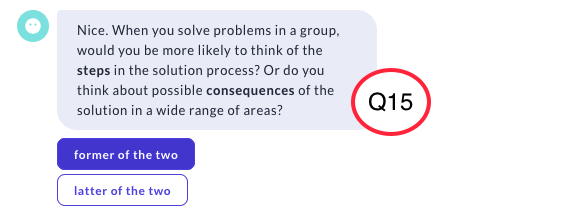
\includegraphics[width=0.7\linewidth]{images/Talk_roterMarker/T15.png}
  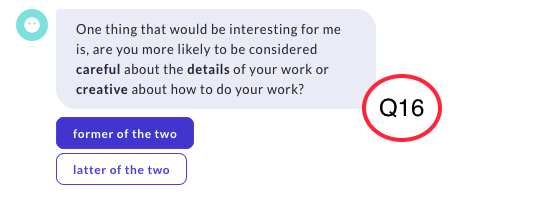
\includegraphics[width=0.7\linewidth]{images/Talk_roterMarker/T16.png}
  
\includegraphics[width=0.7\linewidth]{images/Talk_roterMarker/T17.png}
  \caption[Dialog (1. Interaktion)]{Dialog (1. Interaktion)}
  \label{fig:GesprächIV}
\end{figure} 
Im Folgenden wird eine Übersicht über die von dem Prototypen verwendeten Gestaltungsrichtlinien gegeben.


\textbf{Vorstellung Gestaltungsrichtlinien}  \label{Gestaltungsrichtlinien}

Die folgende Tabelle zeigt die  Gestaltungsrichtlinien, die für die Erstellung des Prototyps, festgelegt wurden.

\begingroup
  \footnotesize                      
  \setlongtables
  \useunder{\uline}{\ul}{}
  \begin{longtable}{|m{4.75cm}|m{3.5cm}|m{1cm}|m{4.75cm}|}
  \hline     
  \rowcolor[HTML]{EFEFEF}  
  
  \centering \textbf{Anforderung} & \centering \textbf{Literaturnachweis} & \centering \textbf{Index} & \centering \arraybackslash \textbf{Gestaltungsrichtlinie}\\ 
  \hline  \hline 

1. Der Prototyp braucht eine Persönlichkeit (z.B. einen Namen). & \parencite[158]{Silvervarg.2012}&GR1& Der Prototyp soll einen heterogenen Namen verwenden.\\ \hline

  2. Der Prototyp benötigt eine visuelle Darstellung. & \parencite[71]{Pearl.2016} &GR2& Der Prototyp soll eine abstrakte und nicht menschenähnliche Visualisierung verwenden. \\ \hline
 
  3. Der Prototyp sollte den Lernenden persönlich ansprechen. & \parencite[60]{Liebrecht.2020} &GR3 & Der Prototyp soll die Lernenden mit ihrem Namen ansprechen.\\ \hline

  4. Der Prototyp sollte menschenähnliche Charackterzüge aufweisen. & \parencite[60]{Liebrecht.2020}, \parencite[9]{Jain.2018} &GR4 & Der Prototyp soll eine alltägliche, informelle und sympathische Sprache imitieren.\\ \hline

  5. Der Prototyp sollte freundlich sein. &\parencite[7]{Wambsganß.2020} &GR5& Der Prototyp soll eine freundliche Ausdrucksweise haben, sodass der Lernende motiviert bleibt. \\ \hline

  6. Der Prototyp benötigt Transparenz und eine verständliche Formulierung. & \parencite[10 f.]{Wambsganß.2021} &GR6& Der Prototyp kann bei Verständnisproblemen des Lernenden seine Aussage anders formulieren. \\ \hline

 7. Der Prototyp sollte eine breite Zugänglichkeit und Benutzerfreundlichkeit sicherstellen, damit Nutzer mit unterschiedlichem Sprach- und Altershintergrund problemlos mit dem CA interagieren können.& \parencite[10 f.]{Wambsganß.2021}, \parencite[9]{Jain.2018} &GR7&Intuitive Kommunikation mit dem CA. Der Prototyp vermittelt dem Lernenden, welche Skills er besitzt.\\ \hline

8. Der Prototyp sollte nicht vorgeben ein Mensch zu sein. & \parencite[1]{villar.2017}, \parencite[1]{neill.2018}&GR8& Der Prototyp soll ehrlich vermitteln, dass er kein Mensch ist. \\ \hline

9. Einbettung eines kausalen Chat-Modus (z.B. über Witze, Wetter) &\parencite[7]{Wambsganß.2020}, \parencite[9]{Jain.2018}&GR9& Sobald der Lernende die Interaktion der Lernstilklassifikation oder die Interaktion des Quizspiels kurz unterbrechen möchte, soll der Prototyp über Chitchatkontexte (Small Talk) verfügen. \\ \hline

10. Der Prototyp sollte über Buttons verfügen. &\parencite[8]{Jain.2018}&GR10&  Der Benutzer soll die Möglichkeit haben über Buttons zu antworten. \\ \hline

11. Der Prototyp sollte eine responsive, einfache und funktionale UX verwenden, damit Studenten das Tool intuitiv nutzen können & \parencite[7]{Wambsganß.2020} &GR11& Die Kommunikation mit dem Prototypen soll über eine dialogbasierte, interaktive, aber einfache, intuitive und übersichtliche Oberfläche laufen.\\ \hline

12. Das Design sollte über einen Typing-Indikator verfügen. & \parencite[10 f.]{Wambsganß.2021} &GR12&  Das Design soll über einen Typing-Indikator verfügen, der die Einhaltung demokratischer sowie moralischer und ethischer Werte signalisiert, um das Fairnessempfinden der Nutzer zu verbessern.  \\ \hline

13. Der Prototyp sollte versuchen beim Quiz-Spiel das scaffolding Verhalten zu imitieren.& \parencite[4 f.]{winkler_hobert_salovaara_söllner_leimeister_2020} &GR13& Der Prototyp soll beim Quiz-Spiel nicht direkt die Antwort verraten, sondern den Lernenden zur Lösung hinführen (scaffolding Verhalten).\\ \hline

\caption[Gestaltungsrichtlinien Prototyp]{Gestaltungsrichtlinien Prototyp (eigene Darstellung)} 
\label{tab:/Gestaltungsrichtlinien_Prototyp} 
\end{longtable}
\endgroup

Die aufgeführten Gestaltungsrichtlinien werden anhand der 
einzelnen Ausschnitte aus dem Dialog
mit dem Prototypen dargestellt. Zum Schluss folgen weitere Gesprächsauszüge zu dem 
Featurizer Count Vector und dem Fallback classifier, welche im Kapitel 4.1 genannt wurden.
Der erste Gesprächsausschnitt verdeutlicht GR1, GR2, GR3 und GR11.
\floatstyle{plain}
\restylefloat{figure}
\begin{figure}[H]
  \centering
  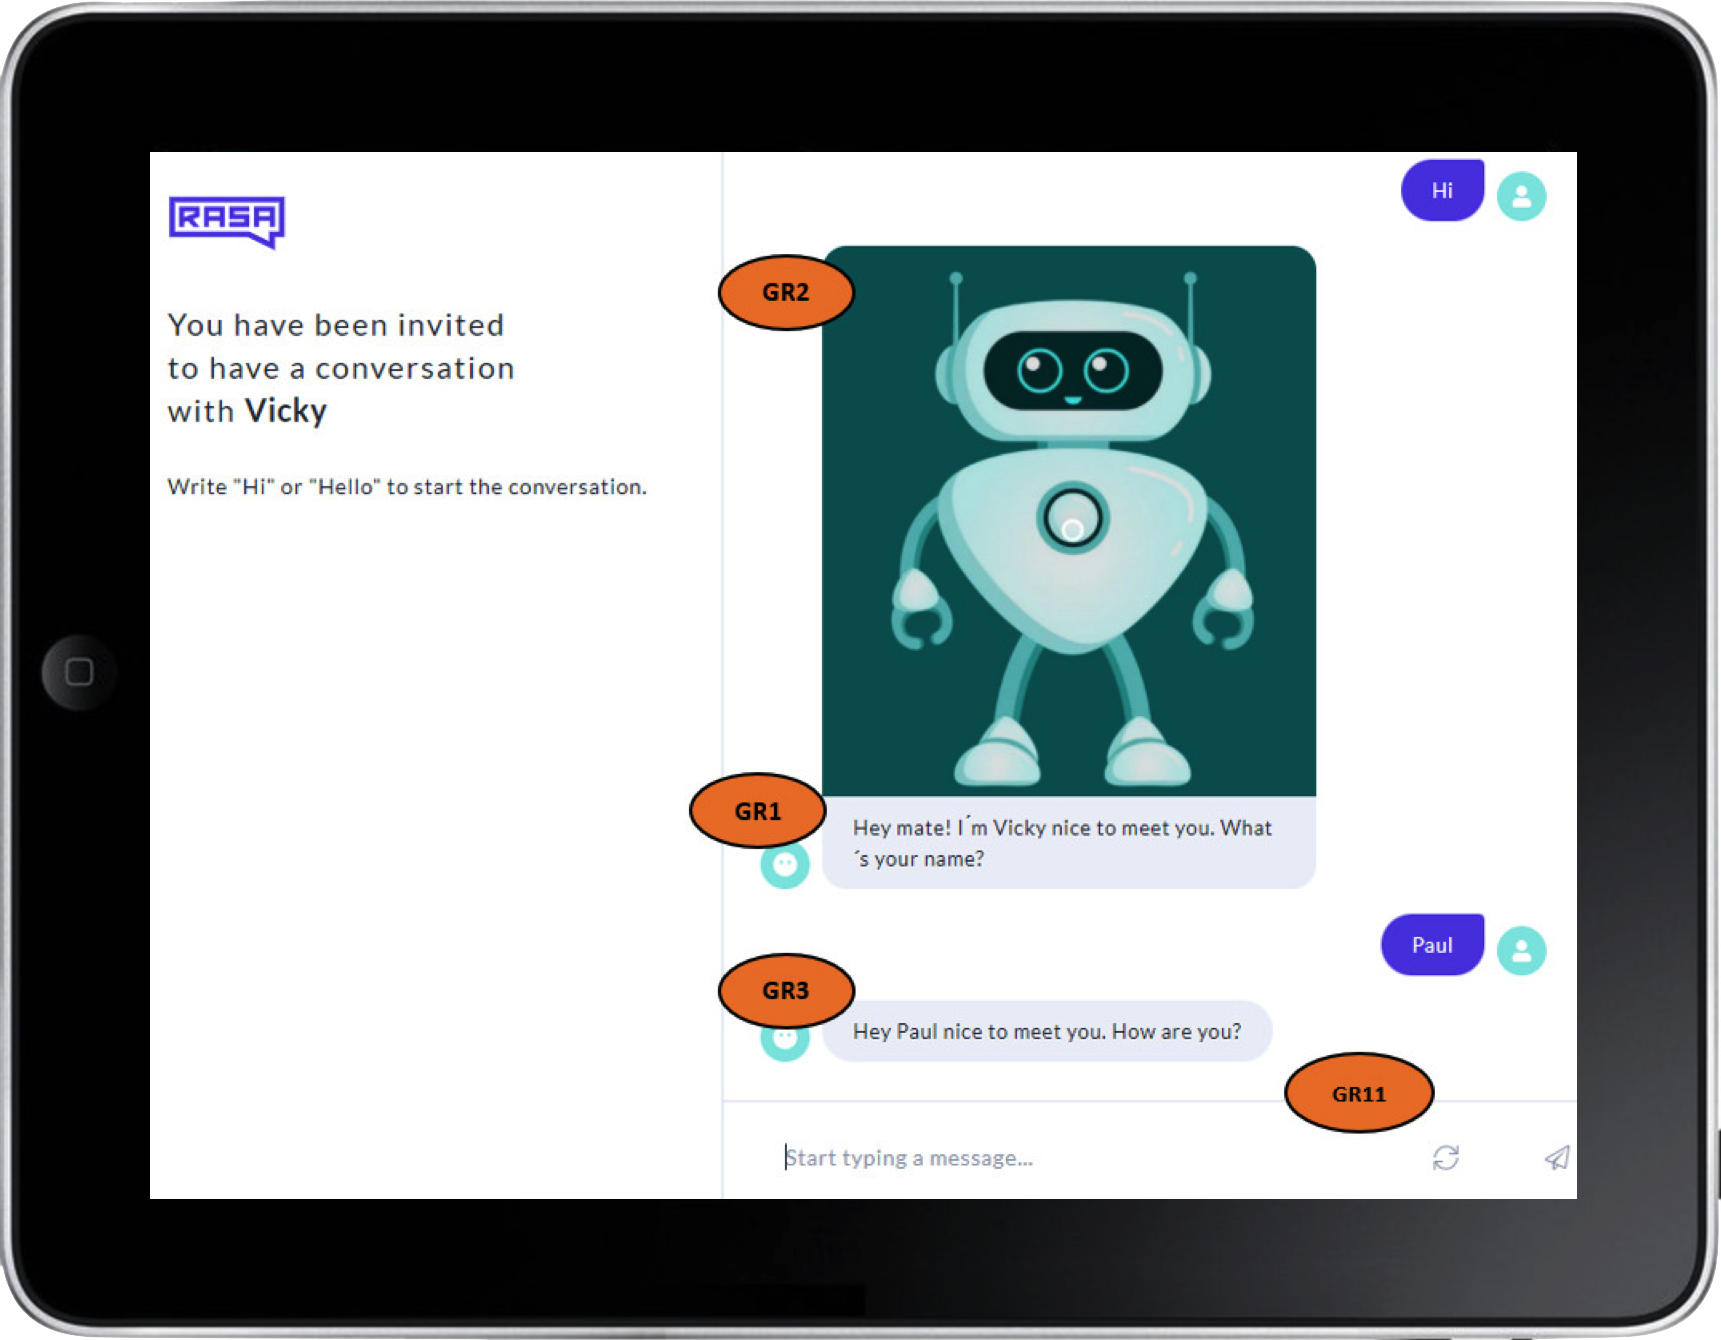
\includegraphics[width=0.85\linewidth]{images/GR1-GR11.png}
  \caption[GR1, GR2, GR3 und GR 11]{GR1, GR2, GR3 und GR11}
  \label{fig:GR1_GR2_GR3_GR11}
\end{figure}
Das erste persönliche Kennzeichen des Prototyps ist, dass er einen heterogen Namen: \textit{Vicky} \footnote{Im Folgenden wird anstelle des Begriffs Prototyp der Name Vicky verwendet.} (GR1) trägt, da Silvervarg u.a. (2012)
herausfanden, das CAs mit einem weiblichen Namen respektloser behandelt und verbal missbraucht werden. \parencite[158]{Silvervarg.2012} 
GR2 fordert eine visuelle Darstellung. Vicky zeigt beim Gesprächsbeginn ein abstraktes und nicht menschenähnliches 
Bild von sich und spricht den Lernenden mit seinem Namen persönlich an (GR3).
Des Weiteren läuft die Kommunikation mit Vicky über eine einfache, 
intuitive und übersichtliche Oberfläche (GR11).

Der nächste Gesprächsausschnitt repräsentiert GR4 und GR10.
\begin{figure}[H]
  \centering
  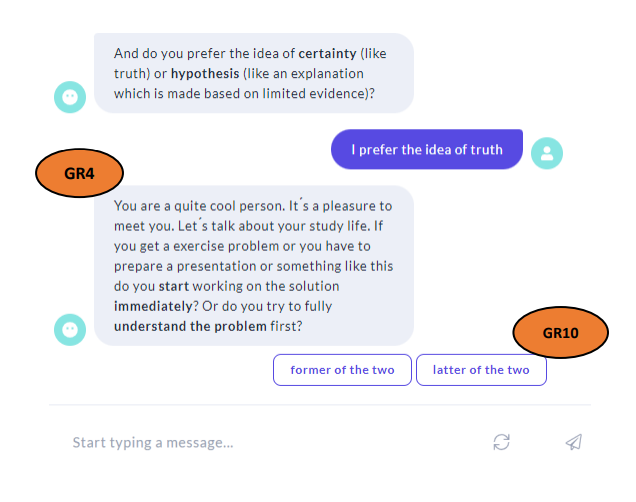
\includegraphics[width=0.7\linewidth]{images/GR4_GR10.png}
  \caption[GR4, GR5 und GR8]{GR4 und GR10}
  \label{fig:GR5_GR4_GR10}
\end{figure}  
Vicky imitiert eine alltägliche, informelle und sympathische 
Sprache (GR4), die beispielsweise durch den Satz: 
\glqq You are a quite cool person ...\grqq{} 
dargestellt wird. Außerdem wird hier das  im Abschnitt 4.1 genannte Beispiel der Synonymverwendung deutlich. 
Es wird nach der \glqq idea of certainty or hypothesis\grqq{} gefragt und 
der Lernende beantwortet die Frage mit  \glqq I prefer the idea of truth\grqq{}.
Das Wort \textit{truth} stellt ein Synonym für \textit{certainty} dar. 
Eine komplette Übersicht über alle verwendeten Synonyme befindet sich im Anhang \ref{SynonymeAnhang}.
Darüber hinaus wird dem Lernenden die Möglichkeit 
gegeben, die letzte dargestellte Frage 
mit der Hilfe von Buttons zu beantworten (GR10). 
\glqq Former of the two \grqq{} bezieht sich auf \glqq I start working on the solution immediately\grqq{}
und \glqq Latter of the two \grqq{} auf \glqq I try to fully understand the problem first\grqq{}.

Ein weiterer Gesprächsausschnitt stellt GR4, GR5 und GR8 dar. 
\begin{figure}[H]
  \centering
  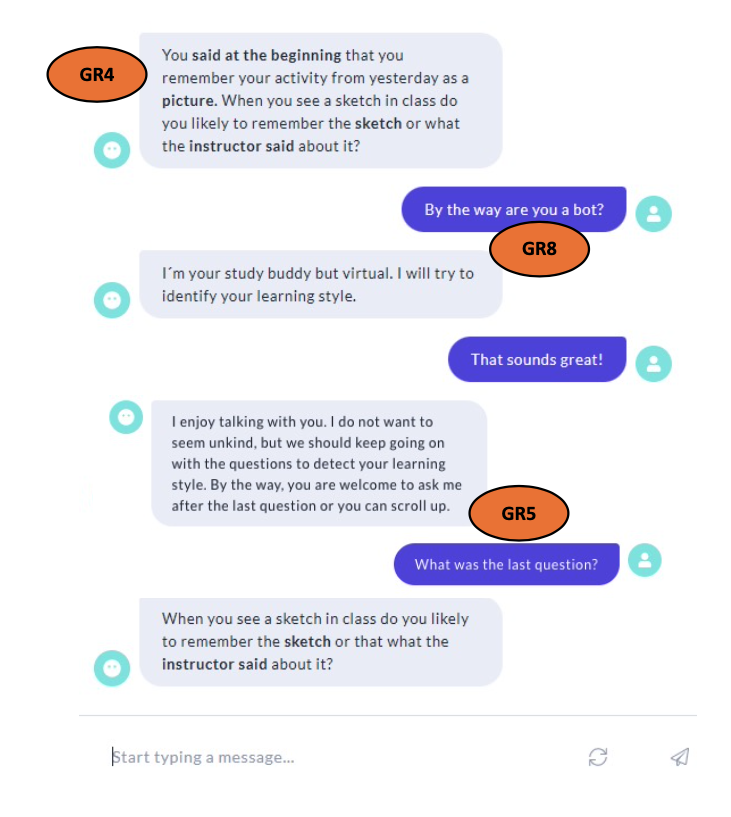
\includegraphics[width=0.7\linewidth]{images/GR4_GR5_GR8.png}
  \caption[GR4, GR5 und GR8]{GR4, GR5 und GR8}
  \label{fig:GR5_GR8_GR4}
\end{figure} 
Vicky beginnt die Frage mit \glqq You said at the beginning that you 
remember your activity from yesterday as a picture.\grqq{}
Hiermit zeigt Vicky Sympathie und  weist ein aktives Zuhören auf (GR4). 
Die gestellt Frage von Vicky bezieht sich auf Q14 (vgl. Tabelle \ref{tab:/Kategorisierung der ILS-Fragen}).
Des Weiteren stellt der Lernende eine Zwischenfrage:
\glqq Are you a bot?\grqq{}, worauf Vickys Antwort verdeutlicht, 
dass Vicky kein realer Mensch ist (GR8). 
Zum Schluss weist Vicky den Lernenden freundlich auf den Hauptdialog
für die Lernstilidentifikation zurück, sodass der 
Lernende weiter motiviert bleibt, die Interaktion mit Vicky
fortzuführen (GR5).
Durch die Möglichkeit, dass der Lernende 
Vicky nach der zuletzt gestellten Frage fragen kann, muss der Lernende 
nicht den Chatverlauf nach oben scrollen.

GR5 und GR9 werden im nächsten Gesprächsausschnitt dargestellt.
\begin{figure}[H]
  \centering
  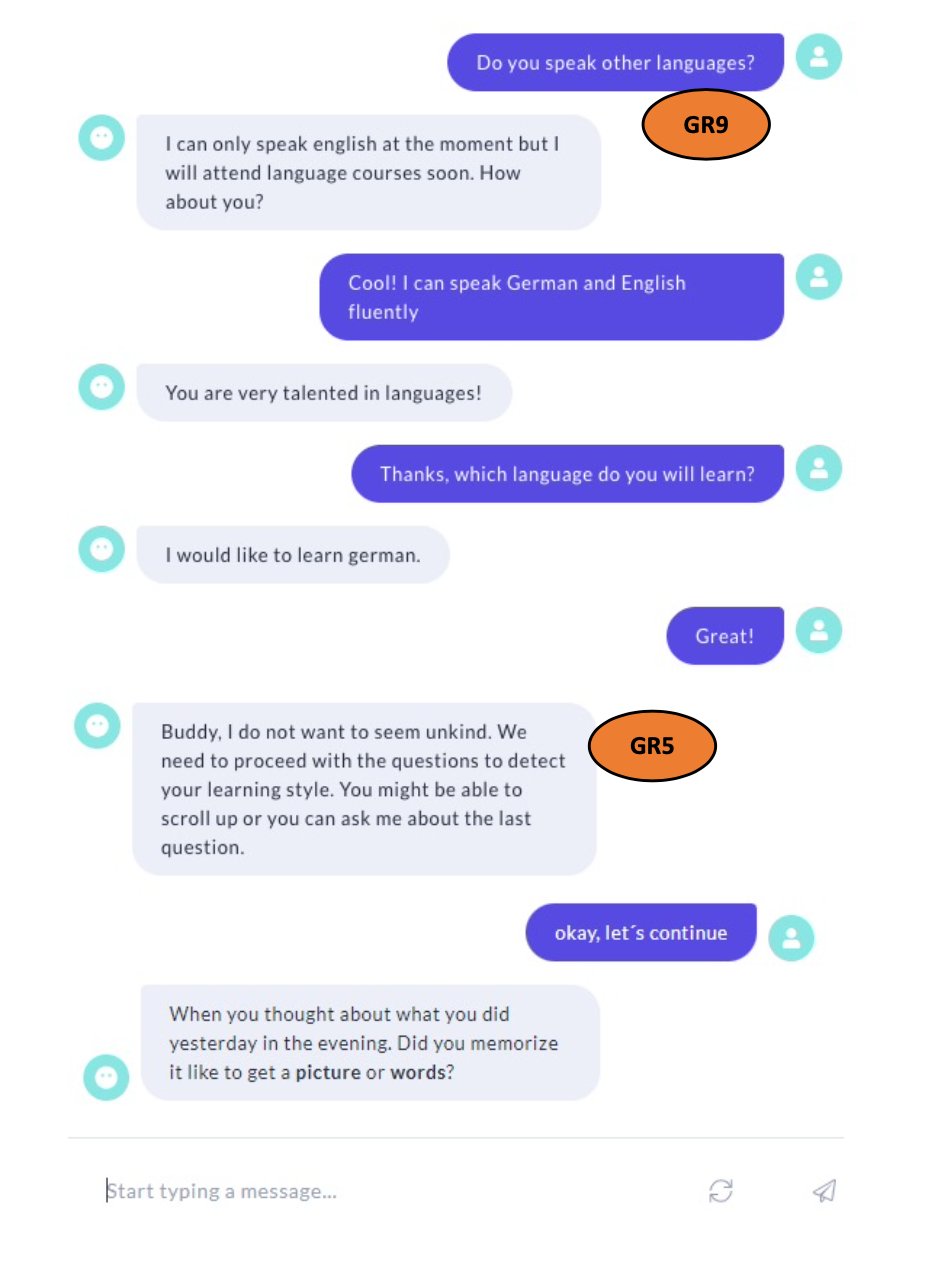
\includegraphics[width=0.7\linewidth]{images/GR5_GR9.png}

  \caption[GR5 und GR9]{GR5 und GR9}
  \label{fig:GR5_GR9}
\end{figure} 
Der Lernende hat die Möglichkeit vom eigentlichen Hauptdialog 
für die Lernstilidentifikation abzuweichen. Er kann kleine Smalltalk-Gespräche mit Vicky führen, sodass er die Gesprächsinteraktion
zur Lernstilklassifikation oder die Interaktion des Quiz-Spiels 
kurz pausieren kann (GR9).
Anschließend führt Vicky den Lernenden wieder freundlich zurück 
auf den Hauptdialog (GR5). Der nächste Gesprächsauszug zeigt GR6 und GR7. 

\begin{figure}[H]
  \centering
  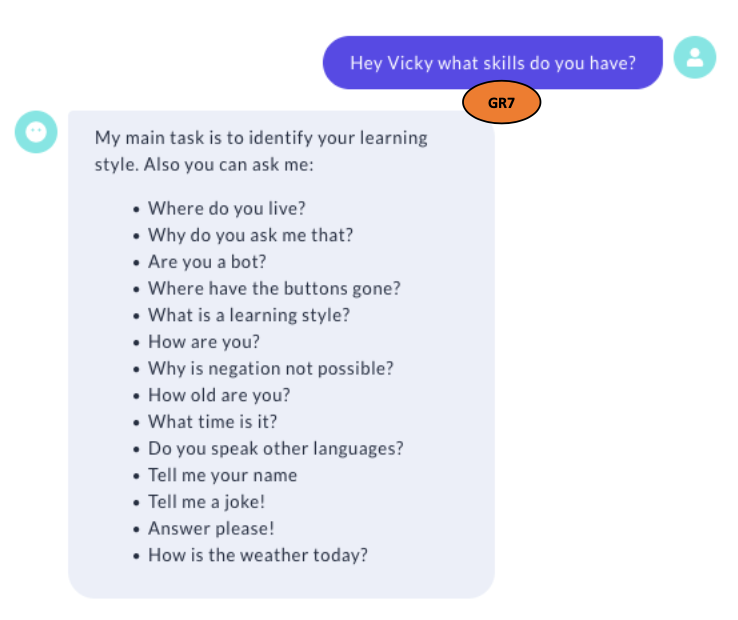
\includegraphics[width=0.7\linewidth]{images/GR67I.png}
  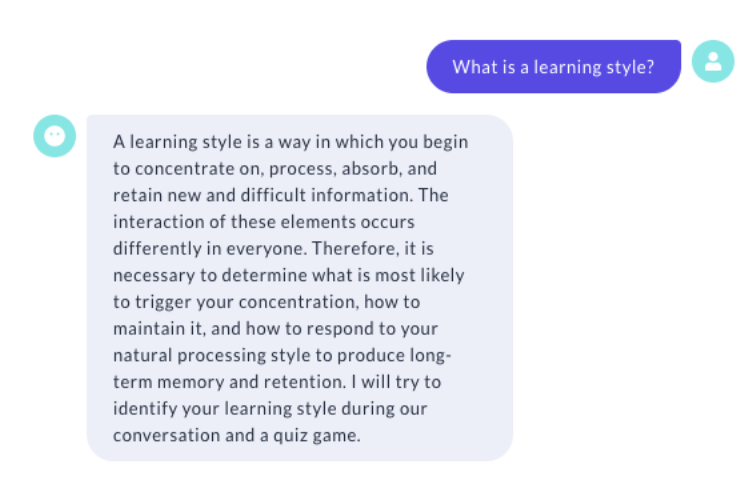
\includegraphics[width=0.7\linewidth]{images/GR67II.png}
  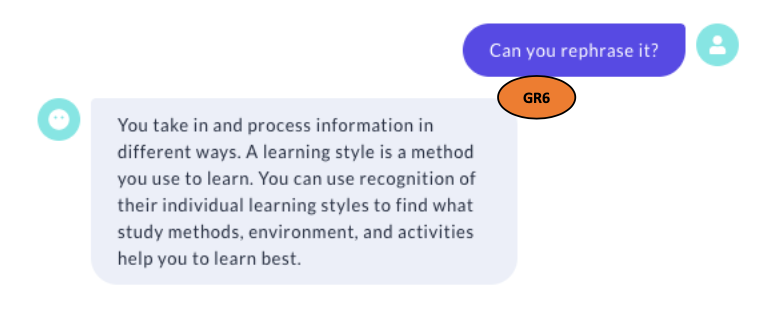
\includegraphics[width=0.7\linewidth]{images/GR67III.png}
  \caption[GR6 und GR7]{GR6 und GR7}
  \label{fig:GR6_GR7}
\end{figure} 


Vicky gibt dem Lernenden eine transparente Auskunft, 
welche Hauptfunktion Vicky hat und auf welche Fragen
Vicky antworten kann. Damit stellt Vicky eine breite Zugänglichkeit 
und Benutzerfreundlichkeit sicher, sodass Lernende mit unterschiedlichem
Sprach- und Altershintergrund problemlos mit Vicky 
interagieren können (GR7). 
Des Weiteren bietet Vicky dem Lernenden die Möglichkeit 
einer Erläuterung zum Lernstil. Ist diese nicht verständlich,
kann der Lernende Vicky fragen, die Antwort anders zu formulieren
(GR6).

Vicky verfügt über einen Typing-Indikator, damit 
der Lernende sieht, ob Vicky aus Fairnessgründen gegenüber 
dem Lernenden antwortet (GR12).
\begin{figure}[H]
  \centering
  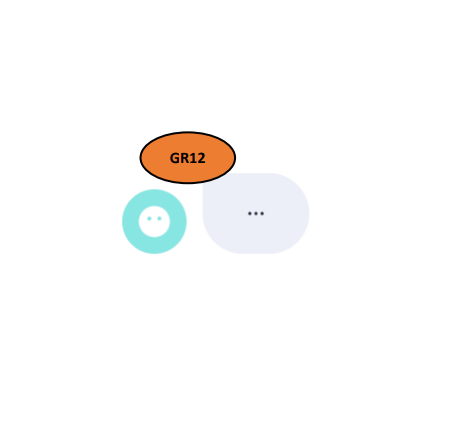
\includegraphics[width=0.35\linewidth]{images/typing.png}
  \caption[GR12]{GR12}
  \label{fig:Typing-Indikator}
\end{figure} 

Die Abbildung \ref{fig:Rechtschreibfehler} zeigt die Rechtschreibfehlerfunktion des Featurizers Count Vectors.
\begin{figure}[H]
  \centering
  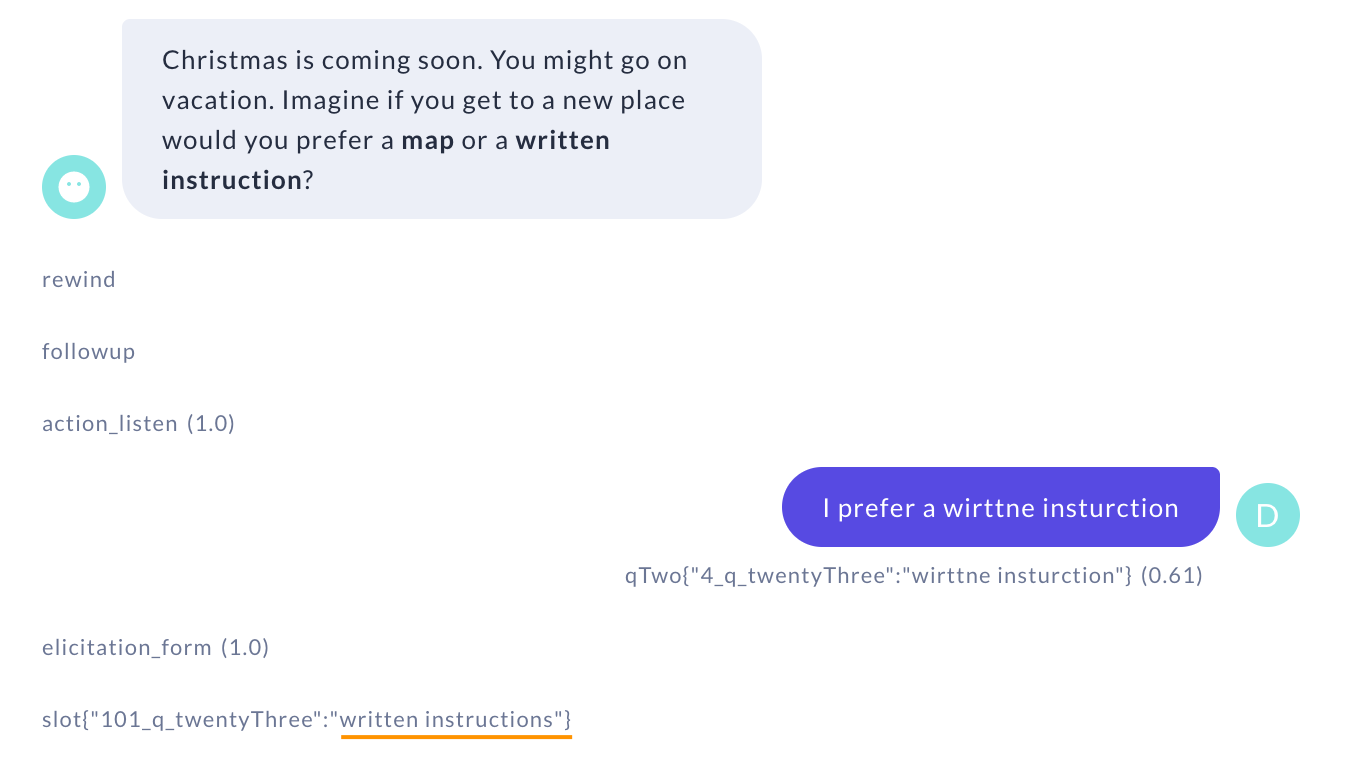
\includegraphics[width=0.8\linewidth]{images/Rechtschreibfehler.png}
  \caption[Rasa X UI (Entwicklersicht): Rechtschreibfehler]{Rasa X UI (Entwicklersicht): Rechtschreibfehler}
  \label{fig:Rechtschreibfehler}
\end{figure} 
Trotz des verschriebenen Wortes \textit{wirttne insturction}, wird die Entity
 \textit{written instructions} identifiziert und als Slot gespeichert, wie 
das orange unterstrichene Wort zeigt. 

Der Fallback classifier
wird in dem folgenden Gesprächsausschnitt dargestellt.
\begin{figure}[H]
  \centering
  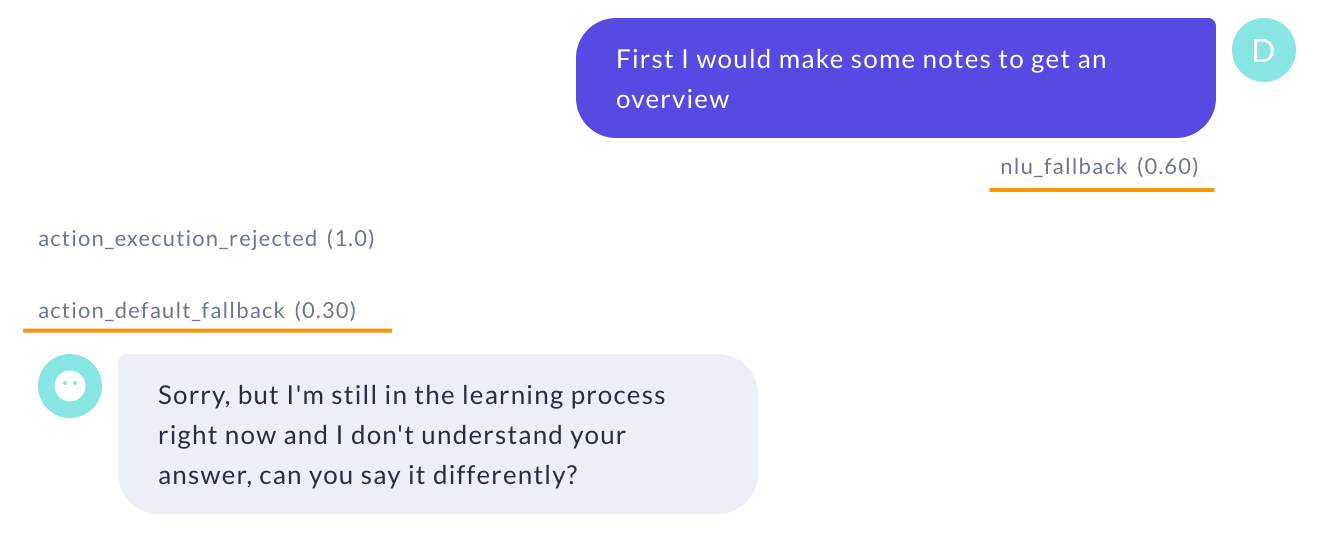
\includegraphics[width=0.85\linewidth]{images/Fallback.png}
  \caption[Rasa X UI (Entwicklersicht): Fallback]{Rasa X UI (Entwicklersicht): Fallback}
  \label{fig:Fallback}
\end{figure} 
Da diese oder ähnliche Formulierung des Satzes 
\glqq First I would make some notes to get an overview\grqq{} 
noch nicht in den Trainingsdaten 
enthalten ist, wird die Fallback Action ausgelöst, welche in der Darstellung 
orange hinterlegt ist. Vicky antwortet anschließend mit einem Ausdruck, der den
Lernenden dazu auffordert, den Satz anders zu formulieren. 
Die Formulierungen \glqq Sorry I didn´t get that. Can you rephrase please?\grqq{}  und \glqq Sorry I didn´t understand, my vocabulary isn´t that developed for that yet. Can you say it in another way?\grqq{} 
stellen weitere Ausdrücke dar, die Vicky bei einer Fallback Action sagen kann. 
Welche Formulierungen Vicky auswählt, wird zufällig von Rasa entschieden.

\subsection{Interaktion: Quiz-Spiel}
Für die Lernstilidentifikation durch eine Art spielerische Komponente (Gamification) wurden
logische Regeln aufgestellt, die helfen, den Lernstil des Lernenden zu klassifizieren.
Im Folgenden werden die Herleitung dieser logischen Regeln, die Fragetypen des 
Quiz-Spiels sowie die ausgewählten Fragen für das Quiz-Spiel und die implementierten
Fragetemplates ausführlich dargestellt.
\pagebreak

\textbf{Logische Regeln}

Latham (2011) hat aus einer Untersuchung 
des ILS-Fragebogens (vgl. Anhang \ref{44ILS}) und der 17 reduzierten Fragen (vgl. Anhang \ref{17-ILS-Fragebogen}) 
herausgefunden, dass 
die Fragen so konzipiert wurden, dass sie die in der Tabelle \ref{tab:/Lernverhaltensmerkmale}
zusammengefassten Verhaltensaspekte testen. Eine vollständige Tabelle der Lernverhaltensmerkmale ist im Anhang \ref{Prototyp_Anhang} zu finden.

\begingroup
\footnotesize 
\begin{longtable}{|m{7.5cm}|m{7.5cm}|}
\hline     
\rowcolor[HTML]{EFEFEF}                                         
\centering \textbf{Lernverhalten beim Lernstil} & \centering \arraybackslash \textbf{Folgerung auf den Lernstil} \\ 
\hline  \hline 
\multicolumn{2}{|c|}{\textbf{sensorisch}} \\ \hline \hline 
Bevorzugen Fakten, Daten, Experimente & Besseres Abschneiden bei Fragen mit Fakten und Beispielen  \\ \hline
Abneigung gegen Überraschungen & Bevorzugen Einführungen in das Thema, Übersichten und die Arbeit in einer sequentiellen vorhersehbaren Reihenfolge \\ \hline
Sorgfältig, aber langsam & Berücksichtigung der Anzahl der Flüchtigkeitsfehler \\ \hline
Vertraut mit Symbolen (z.B. Wörtern) & Umfang der Diskussion mit dem Tutor berücksichtigen\\ \hline  \hline 

\multicolumn{2}{|c|}{\textbf{visuell}} \\ \hline \hline 
Erinnern sich an das, was sie sehen & Besseres Abschneiden bei Fragen mit Diagrammen und Bildern, Filmen \\ \hline
Bevorzugen Bilder und Diagramme & Besseres Abschneiden bei Fragen mit Bildern und Diagrammen \\ \hline
Bevorzugen visuelle Präsentationen & Besseres Abschneiden bei Fragen mit visuellen Erklärungen \\ \hline  \hline   
 

\multicolumn{2}{|c|}{\textbf{verbal}} \\ \hline \hline 
Erinnern sich an das, was sie hören, oder was sie hören und dann sagen & Besseres Abschneiden bei Fragen mit Filmen und Soundclips \\ \hline
Bevorzugen mündliche Erklärung  & Erklärungen des Tutors\\ \hline  \hline   

\multicolumn{2}{|c|}{\textbf{sequentiell}} \\ \hline \hline 
Verfolgen einen linearen Denkprozess, Informationen sollten in einer stetigen Progression von Komplexität gegeben werden &
Bessere Leistung, wenn die Informationen in einem stetigen Grad von Komplexität ansteigen \\ \hline \hline   
 

\multicolumn{2}{|c|}{\textbf{global}} \\ \hline \hline 
Springen direkt zu komplexerem und schwierigem Material &
Sie sind besser, wenn die Informationen zusammengefasst sind, und wenn sie die Aufgaben in einem Durchgang lösen können. \\ \hline
\caption[Lernverhaltensmerkmale und Lernstil (Auszug)]{Lernverhaltensmerkmale und Lernstil (Auszug) (eigene Darstellung, in Anlehnung an \parencite[56]{Latham.2011}) } 
\label{tab:/Lernverhaltensmerkmale} 
\end{longtable}
\endgroup
 

Bei der Betrachtung der Lernverhaltensmerkmale zur Ermittlung des Lernstils  (vgl. Tabelle \ref{tab:/Lernverhaltensmerkmale} \& Anhang \ref{Prototyp_Anhang}) wurde deutlich,
dass jeder Lernstil durch eine kleine Anzahl von Verhaltensweisen kategorisiert werden kann. Zum Beispiel sind sequenzielle Lernende erfolgreicher,
wenn die Informationen schrittweise und mit steigendem 
Schwierigkeitsgrad präsentiert werden, während globale Lernende effektiver lernen, wenn die Informationen zusammengefasst werden und sie 
schwierige Probleme sofort angehen können. Wird dieses Verhalten auf Oscars Nachhilfegespräch angewendet, indem z.B. Fragen eingebaut werden, die den 
Lernenden die Wahl lassen, eine Lösung sofort zu versuchen oder durch Lösungsschritte geführt zu werden, kann der Lernstil 
auf der FS-Dimension sequentiell/global vorhergesagt werden.  \parencite[57]{Latham.2011} 
Die Logik der Klassifikation des Lernstils mithilfe des Quiz-Spiels orientiert sich ebenfalls 
an diesem Vorgehen von Oscar. 

Um die Verhaltensmerkmale in der Tabelle \ref{tab:/Lernverhaltensmerkmale} und in dem Anhang \ref{Prototyp_Anhang} auf Oscars Nachhilfegespräch zur Vorhersage vom persönlichen Lernstil des Lernenden abzubilden,
hat  Latham (2011) die Verhaltensaspekte aus der Tabelle \ref{tab:/Lernverhaltensmerkmale} und aus dem Anhang \ref{Prototyp_Anhang}, je nach Verhalten neu geordnet, 
wobei ähnliche Verhaltensweisen in Gruppen zusammengefasst wurden (vgl. Tabelle \ref{tab:/Lernverhaltenshinweise}). \parencite[57 f.]{Latham.2011}
Anzumerken ist, dass nur die Verhaltenshinweise von Latham (2011) ausgewählt wurden, die für die Logik des
Quiz-Spiels relevant sind.
   

\begingroup
  \footnotesize    
\useunder{\uline}{\ul}{}
\begin{longtable}{|m{7.5cm}|m{7.5cm}|}
  \hline     
  \rowcolor[HTML]{EFEFEF}                                         
  \centering \textbf{Lernverhalten} & \centering \arraybackslash \textbf{ Lernstil} \\ 
  \hline  \hline 
  Richtige Antwort nach dem Betrachten eines Bildes  & visuell                                                       \\ \hline
  Richtige Antwort nach Anschauen eines Videos         & visuell, verbal \\ \hline
  Richtige Antwort nach einer theoretischen Erklärung & intuitiv                                                     \\ \hline
  Richtige Antwort nach dem Betrachten eines Beispiels & sensorisch                                                    \\ \hline
  Schrittweise zur Lösung eines Problems führen lassen & reflektiv, sequentiell \\ \hline
  Direktes Lösen                                                                                 & intuitiv, global   \\ \hline
  Praktische Frage richtig gelöst                                                              & aktiv, sensorisch  \\ \hline
  Theoretische Frage richtig gelöst                                                                & reflektiv, intuitiv \\ \hline
\caption[Lernverhaltenshinweise und Lernstil]{Lernverhaltenshinweise und Lernstil (eigene Darstellung, in Anlehnung an \parencite[58]{Latham.2011})} 
\label{tab:/Lernverhaltenshinweise} 
\end{longtable}
\endgroup     

Zum Beispiel wurde der visuelle und verbale Lernstil dem Lernverhalten \glqq Richtige Antwort nach Anschauen eines Videos\grqq{} 
zugeordnet, da 
sowohl verbale als auch visuelle Lernende bei Fragen mit Filmen besser abschneiden (vgl. Tabelle \ref{tab:/Lernverhaltensmerkmale}).
Ein weiteres Beispiel ist, dass der sensorische Lernstil bei einem Lernverhalten: \glqq Richtige Antwort 
nach dem Betrachten eines Beispiels \grqq{} klassifiziert werden kann, da der sensorische Lerner bei Fragen 
mit Fakten und Beispielen besser abschneidet  (vgl. Tabelle \ref{tab:/Lernverhaltensmerkmale}).

In einem weiteren Schritt hat Latham (2011) diese Verhaltenshinweise in eine Reihe von Logikregeln umgewandelt.
Das Ziel der Logikregeln besteht darin, die Tendenz des Lernstils der Lernenden nach einer Quiz-Frage zu erhöhen. \parencite[70]{Latham.2011}
Es wurden elf Regeln auf Basis von Lathams erstellten logischen Regeln für das Quiz-Spiel erstellt. \parencite[215 f.]{Latham.2011}
Eine vollständige Liste der logischen Regeln ist im Anhang \ref{LogicRulesAnhang} zu finden.
Im Folgenden zeigt das Beispiel die grundsätzliche Idee. 

\begingroup
  \footnotesize  
\begin{enumerate} 
  \item[3)] Bildhilfe:\\
  IF(answer IS(wrong OR don´t know) AND show-image)\\
  THEN\\
  IF(next-answer = right)\\
  THEN\\
  (INCREMENT VISUAL);
\end{enumerate}
\endgroup  

Zum Beispiel repräsentiert die Regel drei, dass der Verhaltenshinweis 
\glqq Richtige Antwort nach Betrachten eines Bildes\grqq{} (vgl. Tabelle \ref{tab:/Lernverhaltenshinweise}) 
mit dem visuellen Lernstil verknüpft wurde.
Weiß der Lernende die Antwort nicht, bekommt aber ein Bild vorgezeigt, welches ihn
auf die richtige Lösung der Frage bringt, bedeutet das, dass diese visuelle Präsentation zum Verständnis
beigetragen hat und sich die Tendenz des Lernenden zu einem visuellen Lernstil erhöht.

In den folgenden Textabschnitten werden die Logischen Regeln weiter erläutert.

\textbf{Fragetypen} \label{Fragetypen}

Latham (2011) verwendet bei Oscars Nachhilfegespräch
vier generische Arten von Fragen. \parencite[70f.]{Latham.2011}
Diese werden ebenfalls für das Quiz-Spiel verwendet:

\begin{minipage}[t]{0.5\textwidth}
\begin{itemize}
  \item Praktischer Typ
  \item Theoretischer Typ
\end{itemize}
\end{minipage}
\begin{minipage}[t]{0.5\textwidth}
  \begin{itemize}
  \item Prozess Typ
  \item Trick Typ \\
\end{itemize}
\end{minipage}

Eine Frage des \textbf{praktischen Typs} bezieht sich auf praktische Probleme und Übungen (z.B. eine Mathematikaufgabe). \parencite[74]{Latham.2011}
Dieser Fragetyp eignet sich für die Bestimmung des aktiven und sensorischen Lernstils (vgl. Tabelle \ref{tab:/Lernverhaltenshinweise}),
da Lernende, welche praktische Aufgaben lösen, dem aktiven Lernstil zugeordnet werden (vgl. Anhang \ref{Prototyp_Anhang}).
Des Weiteren zeigen Lernende mit einem sensorischen Lernstil 
bei Fragen mit Daten und Fakten eine bessere Leistung (vgl. Anhang \ref{Prototyp_Anhang}).
Sobald Lernende eine praktische Frage richtig gelöst haben, erhöht sich die Tendenz zu dem Lernstil aktiv und sensorisch (vgl. Regel 11, Anhang \ref{LogicRulesAnhang}).

Fragen des \textbf{theoretischen Typs} testen das Wissen und das Verständnis der Lernenden. \parencite[74]{Latham.2011} Dieser Fragetyp repräsentiert den 
Lernstil reflektiv und intuitiv (vgl. Tabelle \ref{tab:/Lernverhaltenshinweise}), da Lernende mit diesem Lernstil theoretische Fragen aufgrund einer Affinität zur
Theorie und zu Konzepten besser beantworten können (vgl. Anhang \ref{Prototyp_Anhang}). 
Bei einer richtigen Antwort auf eine theoretische Frage klassifiziert Vicky
die Lernenden in Richtung des reflektiven und intuitiven Lernstils (vgl. Regel 11, Anhang \ref{LogicRulesAnhang}).

Der \textbf{Prozess Typ} zeichnet sich durch Fragen aus, bei denen die Lernenden entweder durch einen Prozess geführt werden oder bei denen sie versuchen können, die Frage im ersten Ansatz zu lösen. \parencite[74]{Latham.2011}
Im ersten Aspekt kann der Lernstil sequentiell und reflektiv klassifiziert werden (vgl. Tabelle \ref{tab:/Lernverhaltenshinweise}), da die Lernenden einen höheren Lerneffekt haben, wenn die Informationen 
in einem stetigen Anstieg von Komplexität und Schwierigkeit präsentiert werden, und sie so die Möglichkeit haben, die Informationen selbständig zu bearbeiten (vgl. Tabelle \ref{tab:/Lernverhaltensmerkmale}, Regel 8, Anhang \ref{LogicRulesAnhang}).
Im zweiten Aspekt kann Vicky den Lernstil intuitiv und global identifizieren (vgl. Tabelle \ref{tab:/Lernverhaltenshinweise}), da die 
Lernenden eine höhere Lernkurve haben, wenn sie auf der Basis von
zusammengefassten Informationen komplexe und schwierige Aufgaben direkt lösen können (vgl. Tabelle \ref{tab:/Lernverhaltensmerkmale}, Regel 7, Anhang \ref{LogicRulesAnhang}).

Bei Fragen des \textbf{Trick Typs} ist die Antwort zum Teil im Beschreibungstext enthalten.
Es soll getestet werden, wie aufmerksam die Lernenden lesen. \parencite[74]{Latham.2011}
Vicky kann durch diesen Fragetyp zum einen den sensorischen und verbalen und zum anderen 
den intuitiven und visuellen Lernstil klassifizieren (vgl. Regel 10, Anhang \ref{LogicRulesAnhang}).
Die erste Annahme trifft zu, wenn die Lernenden die Frage des Trick Typs im ersten Versuch richtig beantworten, 
da Lernende dieser Lernstilkategorie einen aufmerksamen und sorgfältigen Bearbeitungsstil bevorzugen. Außerdem
zeigen sie eine Affinität zu Wörtern (vgl. Anhang \ref{Prototyp_Anhang}).
Die zweite Annahme trifft zu, wenn die Lernenden mehrere Versuche für die richtige Antwort benötigen, 
da sie keinen sicheren Umgang mit unbekannten Wörtern aufweisen, sondern eher eine starke Affinität zu visuellen Materialien (z.B. Diagrammen oder Bildern) aufzeigen (vgl. Anhang \ref{Prototyp_Anhang}).

Latham (2011) absolvierte weitere Experimente, um unter anderem die Lernstilklassifikation durch 
die Fragestile sowie die aufgestellten logischen Regeln
zu validieren. Vor der Interaktion mit Oskar haben die Teilnehmer den ILS-Fragebogen 
ausgefüllt. Drei der vier FS-Dimensionen waren ungefähr gleich verteilt. Bei der Dimension visuell/verbal gab es 
viel mehr visuelle als verbale Lernende. Dies hatte auf die Ergebnisse der weiteren Analyse Auswirkungen.
An den Ergebnissen des ILS-Fragebogens konnte dann geprüft werden, ob Oscar den Lernstil erfolgreich klassifizieren konnte. \parencite[118]{Latham.2011}
Mit dem Experiment wird der Erfolg eines Teilnehmers bei der Beantwortung verschiedener Arten von Übungsfragen
betrachtet um so einen Lernstil vorauszusagen. 
Teilnehmer, die bei theoretischen Fragen besser abschneiden, werden als reflektiv und intuitiv eingestuft, Probanden, die
bei praktischen Fragen ihre Stärke haben, werden als aktiv und sensorisch eingestuft (vgl. Regel 11, Anhang \ref{LogicRulesAnhang}).
Es gab 70 Teilnehmer, die eine Vorliebe für praktische oder theoretische
Übungsfragen zeigten. Die Teilnehmer, die bei beiden Fragestilen gleich erfolgreich waren, blieben unklassifiziert.
Oscar  war nicht in der Lage, den sensorischen Lernstil vorherzusagen. Der erfolgreichste Faktor bei der Vorhersage
war der reflektive Lernstil. \parencite[123]{Latham.2011} \\
Bezüglich der Validierung der logischen Regeln konnte Oscar den globalen und reflektiven Lernstil nicht klassifizieren.
Die Merkmale des reflektierenden Lerners legen nahe, dass sie nach dem Lernen Zeit aufwenden müssen, um über
das neue Wissen nachzudenken.
Da diese Aktivität nach dem Lernen stattfindet, ist es nicht möglich, einen reflektierenden Lernstil während eines Tutoriums vorherzusagen.
Dennoch war die Vorhersage von intuitiv, aktiv und sequentiell erfolgreich. Aufgrund von einer ungleichen Verteilung der Teilnehmer 
für die FS-Dimension visuell/verbal war eine Klassifikation nicht möglich. \parencite[121 f.]{Latham.2011}
Somit wird erstes Potenzial für die Lernstilklassifikation mithilfe der Fragestile und der logischen Regeln nachgewiesen.

\textbf{Fragenauswahl für das Quiz-Spiel}\label{Fragenauswahl}

Für die Beantwortung der Fragestellung RQ1 wird auf alle Lernenden verwiesen, sodass Vicky den Lernstil nicht 
von Lernenden eines bestimmten Studiengangs klassifizieren soll, sondern allgemein Lernende sollen als Zielgruppe 
betrachtet werden, Lernende in einer beruflichen Weiterentwicklung, Schüler oder Studierende.  
Um die passenden Fragen für diese Zielgruppe zu finden, wurde auf Knobelaufgaben und Fragen zum Allgemeinwissen 
zurückgegriffen. Dadurch soll eine Unabhängigkeit zum Studiengang des Lernenden geschaffen werden. 
Auf Basis der Literatur wurden Fragen ausgewählt und zum Teil abgeändert. Beispielsweise wurden bei mathematischen Aufgaben 
anstatt normaler Zahlen 
römische Zahlen genutzt. Solche Änderungen wurden vorgenommen, damit zum einen Vicky bessere Hilfestellung 
während des Quiz-Spiels geben kann und
zum anderen hätten mehrere Fragen, bei denen die Antworteingaben mit numerischen Zahlen erforderlich waren,
zu einer schlechteren Klassifikation der Intents von Vicky geführt. Eine vollständige Liste 
der ausgewählten Fragen sind im Anhang \ref{FragenQuizSpiel} vorzufinden.
Auf der Meta-Ebene werden die Fragen zwischen theoretischem und praktischem Typ unterschieden.
Die Fragen 1, 4, 5 und 8 werden dem theoretischen Typen zugeordnet. Dabei sind Frage 1 und 5 ebenfalls von der Kategorie Trick Fragen.
Die Fragen 2, 3, 6 und 7 werden als Fragen des praktischen Typs kategorisiert. Darunter sind die Fragen 3 und 6 ebenfalls Fragen des Prozesstyps.

\textbf{Fragetemplates} 

Für das Quiz-Spiel wurden zwei verschiedene Fragetemplates entwickelt. 
Die folgende Abbildung \ref{fig:Fragetemplate_I} zeigt das erste Fragetemplate mit Lösungshinweisen, welche die Fragen eins, zwei, vier, fünf,
sieben und acht betreffen (vgl. Anhang \ref{FragenQuizSpiel}). 
\begin{figure}[H]
  \centering
  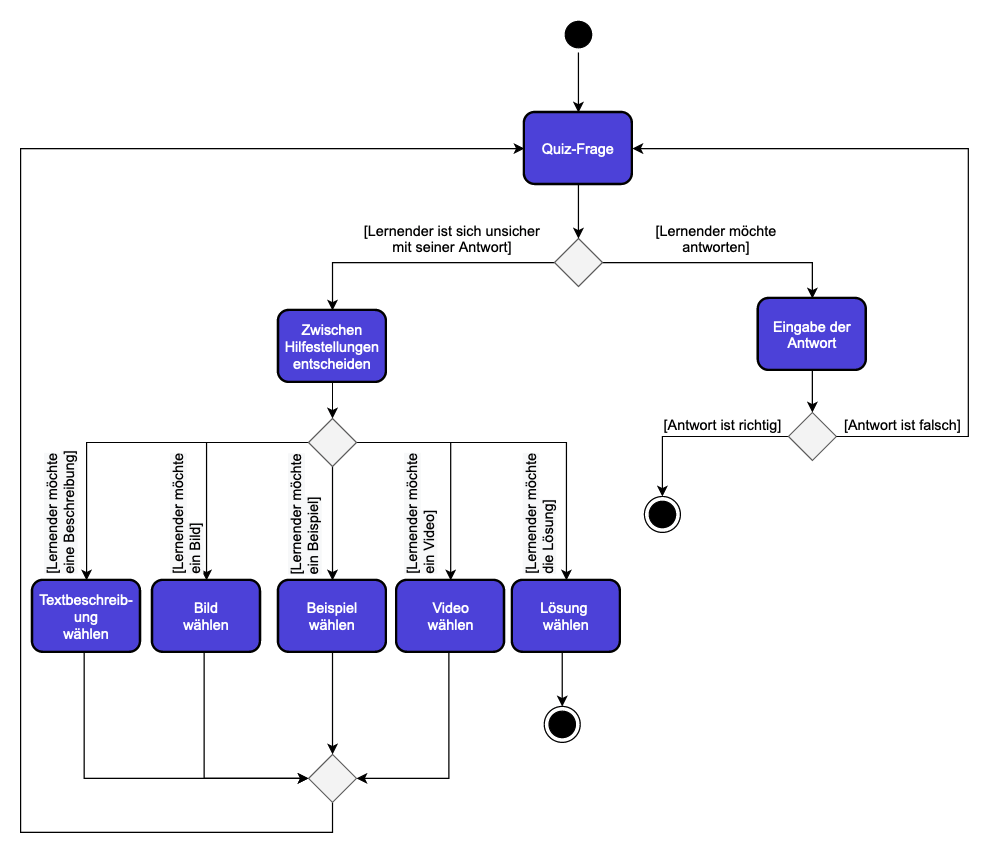
\includegraphics[width=0.85\linewidth]{images/temI.png}
  \caption[Fragetemplate I]{Fragetemplate I  (eigene Darstellung)}
  \label{fig:Fragetemplate_I}
\end{figure} 


Zu Beginn stellt Vicky dem Lernenden die Quiz-Frage. 
Der Lernende kann entweder direkt antworten oder er fordert Unterstützung von Vicky über einen 
Hilfsbutton an.
Möchte der Lernende direkt antworten, kann er die Antwort im Textfeld eintippen.
Anschließend wird geprüft, ob die Frage korrekt beantwortet wurde. Im Falle einer richtigen Antwort teilt Vicky dem Lernenden mit,
dass er die Frage richtig beantwortet hat und fügt eine kleine Erklärung dazu, warum die Antwort richtig ist. Anschließend 
fährt Vicky mit der nächsten Frage fort.
Im Falle einer falschen Antwort sagt Vicky dem Lernenden, dass er die Frage falsch beantwortet hat und 
stellt die Frage nochmal. Nun kann der Lernende sich wieder zwischen einer direkten Antwort oder einer Reihe von 
verschiedenen Hilfestellungen entscheiden. Möchte der Lernende Hilfe von Vicky bekommen, kann der Lernende
zwischen verschiedenen Buttons mit unterschiedlicher Hilfsfunktion wählen. 
Wählt der Lernende den Button mit der Hilfe der Textbeschreibung, bekommt der Lernende eine 
überschaubare textuelle Beschreibung als Lösungshinweis zur Frage. 
Bei einer Wahl des Buttons mit einer Beispielvorlage wird dem Lernenden bezüglich der Frage
ein ähnliches Beispiel gezeigt. Anhand dieses Beispiels kann der Lernende die Antwort von der Ausgangsfrage
ableiten.
Sofern der Lernende den Button mit einer Hilfestellung als Bild oder als Video gewählt hat, schickt Vicky dem Lernenden 
einen visuellen Lösungshinweis. 
Nach der Auswahl eines der vier Hilfestellungen wird dem Lernenden die Ursprungsfrage angezeigt und dieser kann erneut 
entweder direkt antworten oder eine andere Hilfsoption wählen. 
Beantwortet der Lernende die Frage nach der letzten ausgewählten Hilfsoption richtig, bestimmen die aufgestellten 
Regeln (vgl. Anhang \ref{LogicRulesAnhang}), welche Lernstiltendenz sich erhöht hat.\\
Die \textbf{Quiz-Frage eins} ist dem Typen Theorie und Trick zugeordnet, 
beantwortet der Lernende nun die Quiz-Frage falsch, kann er
z.B. die Hilfestellung \textit{Bild} wählen und bekommt eine bildliche Darstellung
des Problems.
Beantwortet der Lernende nach dem visuellen Hinweis die Frage jedoch richtig, 
gelten die Regeln drei, zehn und elf,
da erstens die letzte Hilfsoption, die der Lernende ausgewählt hat, von visueller Art war, zweitens 
die Frage vom theoretischen und Trick Typ ist. 
Somit steigt die Tendenz des Lernenden zum Lernstil zweimal visuell, zweimal intuitiv und reflektiv. 

Je nachdem mit welcher Hilfsoption der Lernende die Antwort beantwortet hat, gilt die dazugehörige Regel.
In diesem Beispiel war es die Hilfestellung per Bild und somit galt die Regel drei. Hätte der Lernende 
die Frage aufgrund einer Hilfestellung per textueller Beschreibung beantwortet, hätte anstatt der Regel drei die Regel eins 
gezählt, per Video die Regel zwei und per Beispiel die Regel vier.
Beantwortet der Lernende die Frage im ersten Versuch ohne jegliche Hilfestellung, würde anstatt der Regel drei die Regel sieben gelten.

Die Abbildung \ref{fig:Fragetemplate_II} zeigt das zweite Fragetemplate für die Quiz-Fragen drei und sechs, welche vom praktischem und Prozess Typ sind
(vgl. Anhang \ref{FragenQuizSpiel}). 
\begin{figure}[H]
  \centering
  \includegraphics[width=0.9\linewidth]{images/templateII.png}
  \caption[Fragetemplate II]{Fragetemplate II  (eigene Darstellung)}
  \label{fig:Fragetemplate_II}
\end{figure} 
Nachdem die Quiz-Frage gestellt wurde, kann der Lernende entweder direkt antworten oder er fordert über den 
Hilfsbutton einen geführten Prozess zur Lösung an. Bei einer direkten Antwort des Lernenden wird die Antwort geprüft,
und Vicky gibt dem Lernenden eine Rückmeldung, ob seine Antwort richtig oder falsch war. Bei einer richtigen Antwort 
fährt Vicky nach der Erklärung, warum die Antwort richtig ist, mit der nächsten Frage fort. 
Bei einer falschen Antwort kehrt er zur Frage zurück und kann erneut zwischen direkter Antwort oder der Hilfestellung von 
Vicky wählen. 
Bei der Wahl über die Hilfestellung gibt Vicky dem Lernenden einen Hinweis sowie eine Zwischenfrage, welche die 
Ermittlung der Antwort auf die Ausgangsfrage unterstützt. Im Falle einer richtigen Antwort zur Zwischenfrage wird der Lernende 
zur Ausgangsfrage zurückgeleitet und kann auf diese antworten. 
Im Falle einer falschen Antwort gibt Vicky dem Lernenden einen weiteren Lösungshinweis und stellt die Zwischenfrage erneut.
Nachdem der Lernende erneut eine Antwort auf die Zwischenfrage gegeben hat, unabhängig von einer richtigen oder falschen Antwort,
kommt er nach der Erklärung der Antwort auf die Zwischenfrage zur Ausgangsfrage zurück und kann die Ausgangsfrage beantworten.\\
Zum Beispiel ist \textbf{Quiz-Frage drei} als praktischer und Prozess Fragetyp kategorisiert.
Beantwortet der Lernende die Frage direkt richtig, 
gelten die Regeln sechs, sieben und elf, da er erstens die Frage im ersten Ansatz richtig beantwortet hat, zweitens er sich dafür entschieden hat, die Frage ohne Hilfestellung
zu beantworten und drittens die Ausgangsfrage vom praktischen Prozess Fragetyp ist. Daher erhöht sich seine Tendenz zum Lernstil zweimal intuitiv, zweimal global, 
aktiv und sensorisch (vgl. Anhang \ref{LogicRulesAnhang}).
Beantwortet der Lernende zuerst die Ausgangsfrage falsch und wählt die Hilfsoption,
wird der Lernende durch einen Hinweis und eine Zwischenfrage zur Lösung der Ausgangsfrage 
geführt. Beantwortet er durch diese Hilfeleistung die Ausgangsfrage richtig, gelten die Regeln acht, neun und elf, da
der Lernende sich für einen schrittartigen und geführten 
Prozess entschieden hat sowie die Ausgangsfrage vom praktischem und Prozess Fragetyp ist. 
Also erhöht sich die Tendenz des 
Lernenden zum Lernstil zweimal sequentiell, reflektiv, sensorisch, verbal und aktiv (vgl. Anhang \ref{LogicRulesAnhang}).


Allgemein soll Vicky nicht sofort die richtige Antwort geben, sondern versuchen dem Lernenden zu helfen, 
das fehlende Wissen aufzubauen und selbständig die Lösung zu finden.
Dies wird auch als scaffolding Verhalten bezeichnet, 
was der CA Sara von Winkler u.a. (2020) ebenfalls versucht zu imitieren.
Des Weiteren gilt für beide Fragetemplates, dass sobald der Lernende die Frage nicht im ersten Versuch richtig beantwortet, die Regel sechs entfällt und beim 
zweiten Fragetemplate die Regel neun ergänzt wird, da bei mehreren Versuchsantworten sich eine Tendenz zu dem Lernstil sequentiell und verbal aufbaut.
Regel fünf \glqq Kleine Fehler\grqq{} ist nur bei der Quiz-Frage sieben von Bedeutung, da der Lernende dort drei Antworten geben muss.
Der Prototyp gibt dem Lernenden Rückmeldung, welcher Antwortenteil richtig ist, und kann anschließend versuchen die Aufgabe 
nochmal zu beantworten. Gilt Regel fünf, erhöht sich die Lernstiltendenz des Lernenden zu intuitiv aufgrund der Neigung
zu flüchtigem Arbeiten des Lernenden (vgl. Anhang \ref{Prototyp_Anhang}).
Darüber hinaus erklärt Vicky immer die Antwort auf die Frage unabhängig davon, ob der Lernende 
die Frage richtig oder falsch beantwortet hat. Dies ist ein weiteres Kennzeichen des scaffolding Verhaltens. \parencite[4 f.]{winkler_hobert_salovaara_söllner_leimeister_2020}
Des Weiteren stellt Vicky zu jedem Fragetemplate einen Lösungsbutton. Allerdings wird beim Drücken des Lösungsbuttons kein 
Lernstil für diese Frage ermittelt. 

\textbf{Vorstellung Quiz-Spiel}

Der Lernende startet das Spiel durch das Klicken auf den Button \glqq Let´s play!\grqq{}.
Vicky stellt ihm zu Beginn vier Fragen. Jede Frage spiegelt einen bzw. zwei Fragetypen (siehe Teilabschnitt: Fragetypen, S. \pageref{Fragetypen})
wider. Nachdem Vicky dem Lernenden vier Fragen gestellt hat, fragt Vicky ihn, ob er das Spiel beenden möchte
oder noch weiterspielen möchte. Im ersten Fall ist die zweite Interaktion Quiz-Spiel zwischen dem Lernenden und 
Vicky beendet. Im zweitem Fall stellt Vicky dem Lernenden vier weitere Fragen. 
Die nächste Abbildung zeigt einen Auszug vom Spielbeginn sowie der ersten Quiz-Frage (vgl. Anhang \ref{FragenQuizSpiel}).
\begin{figure}[H]
  \centering
  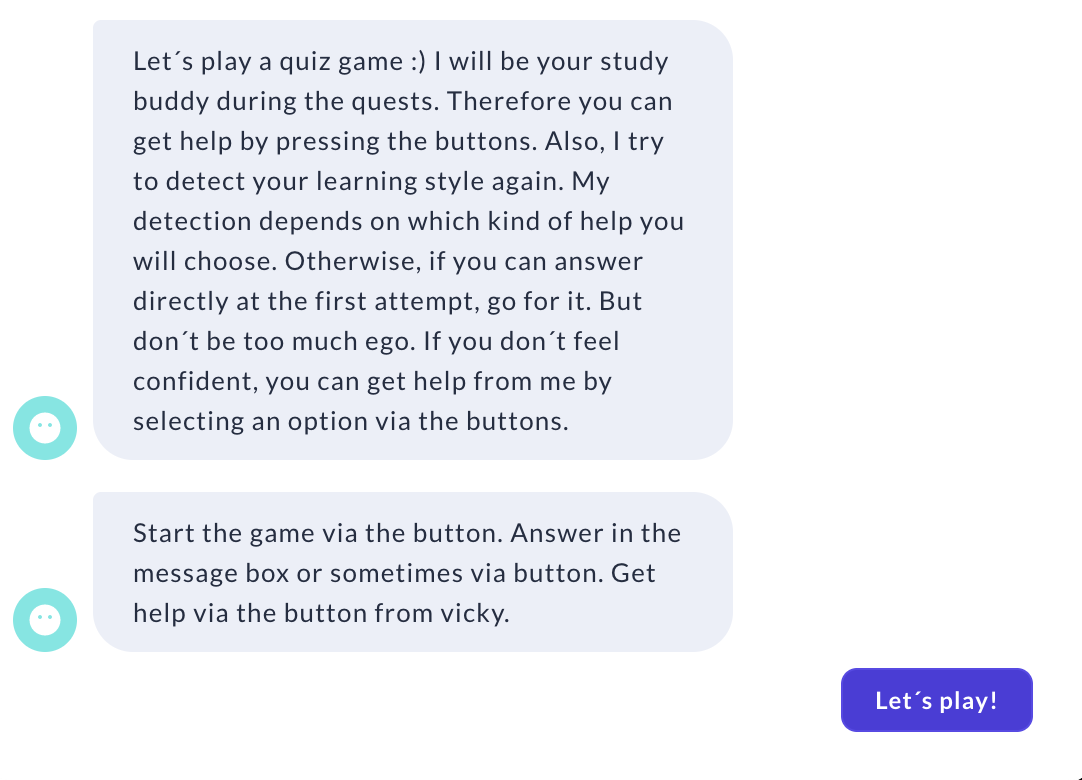
\includegraphics[width=0.65\linewidth]{images/VickyQuiz/gamestart.png}
  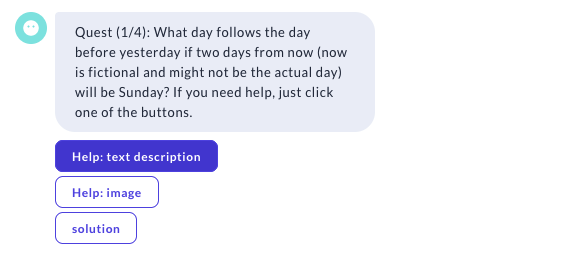
\includegraphics[width=0.65\linewidth]{images/game/q1.png}

\end{figure}
\begin{figure}[H]
  \centering 
  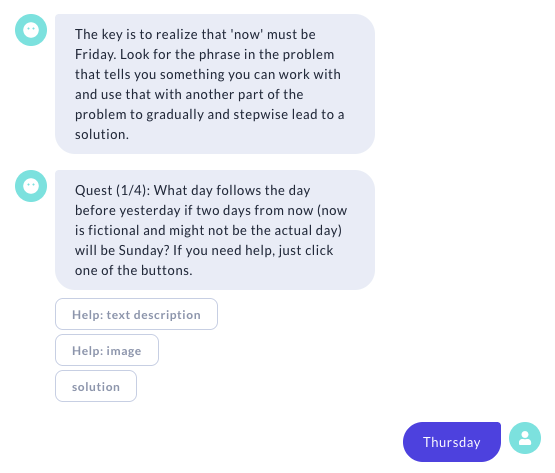
\includegraphics[width=0.7\linewidth]{images/game/q1.1.png}
  
\includegraphics[width=0.7\linewidth]{images/game/q1.2.png}

  \caption[Quiz-Spiel: Spielbeginn und 1. Quiz-Frage]{Quiz-Spiel: Spielbeginn und 1. Quiz-Frage}
  \label{fig:Spielbeginn_und_1._Quiz-Frage}
\end{figure} 
Nachdem der Lernende das Spiel gestartet hat, stellt Vicky ihm die erste Quiz-Frage.
In diesem Fall wählt der Lernende eine Hilfestellung per textueller Beschreibung.
Nachdem er den Hinweis gelesen hat, beantwortet er die Frage. Anschließend 
gibt Vicky ihm eine Rückmeldung über seine Antwort und erklärt die richtige Antwort,
unabhängig davon, ob er die Frage richtig oder falsch beantwortet hat.
Aufgrund der richtigen Antwort im ersten Anlauf des Lernenden, der Hilfestellung per textueller
Beschreibung und der Art der Frage (theoretischer und Trick Typ) erhöht sich die 
Lernstiltendenz des Lernenden zu viermal intuitiv, global, visuell und reflektiv (vgl. Anhang \ref{LogicRulesAnhang}, Regeln 1, 6, 10 und 11).

Der zweite Auszug aus dem Quiz-Spiel zeigt die dritte Quiz-Frage (vgl. Anhang \ref{FragenQuizSpiel}).
\begin{figure}[H]
  \centering
  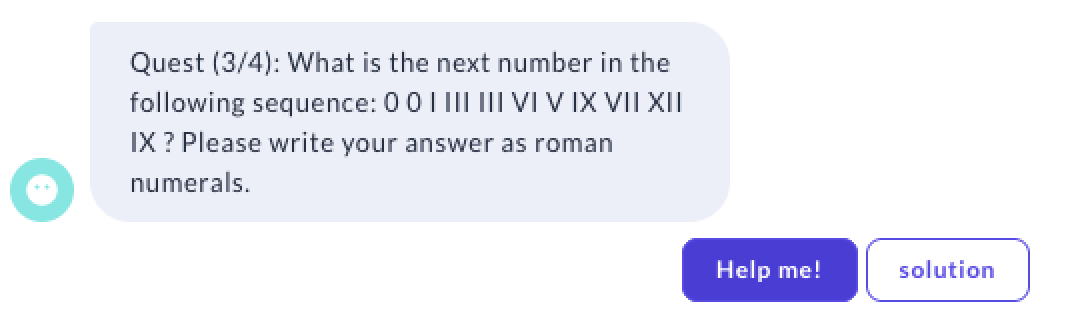
\includegraphics[width=0.7\linewidth]{images/VickyQuiz/Q2.2.png}
  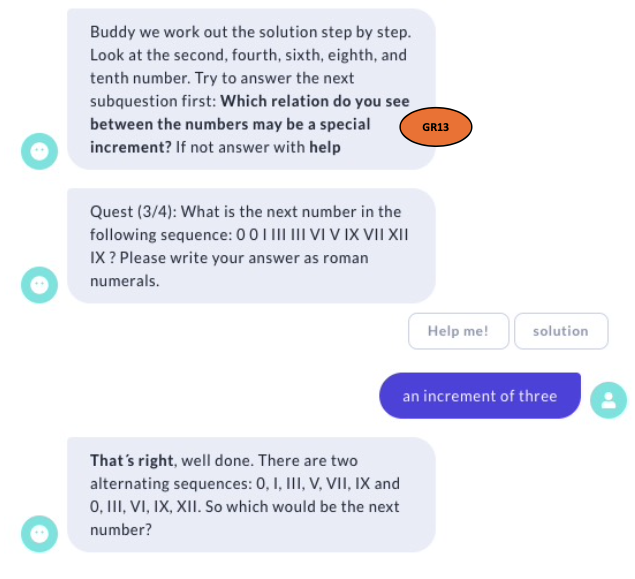
\includegraphics[width=0.7\linewidth]{images/Game/q3.01.png}
  
\includegraphics[width=0.7\linewidth]{images/VickyQuiz/q4.1.png}
  
\includegraphics[width=0.7\linewidth]{images/VickyQuiz/q4.2.png}
  \caption[Quiz-Spiel: 3. Quiz-Frage]{Quiz-Spiel: 3. Quiz-Frage}
  \label{fig:3._Quiz-Frage}
\end{figure}  


Der Lernende entscheidet sich für einen geführten Prozess zur Lösung.
Nachdem er den Hilfsbutton gedrückt hat, bekommt er einen Lösungshinweis 
sowie eine Zwischenfrage, welche er zuerst beantworten muss. Hier kennzeichnet sich das Scaffolding Verhalten (GR13). Vicky versucht den Lernenden zur Lösung hinzuführen. 
Nachdem der Lernende diese beantwortet hat, gibt Vicky ihm 
eine erklärende Rückmeldung bezüglich seiner richtigen Antwort. Anschließend kann der Lernende 
die Ausgangsfrage versuchen zu beantworten. 
Nachdem er eine 
richtige Antwort auf die Ausgangsfrage abgegeben hat, 
gibt Vicky ihm eine Rückmeldung und eine Erklärung der richtigen Antwort.
Die Lernstiltendenz des Lernenden erhöht sich aufgrund seiner richtigen Antwort 
im ersten geführten Prozess von Vicky und der darauffolgenden Fragearten: praktisch und Prozess zu 
intuitiv, global, sequentiell, reflektiv, sensorisch und aktiv (vgl. Anhang \ref{LogicRulesAnhang}, Regeln 6, 8 und 11).

Ein kompletter Spielablauf ist im Anhang \ref{AusschnitteQuizSpiel} vorzufinden.

\textbf{Lernstilerläuterung}

Vicky bestimmt den Lernstil nach jeder Interaktion mit dem Lernenden.
Nachdem Vicky den Lernstil nach dem Dialog
bestimmt hat, gibt Vicky dem Lernenden seine Einschätzung und fragt den 
Lernenden, ob er eine ausführlichere Erklärung zu seinem 
Lernstil haben möchte. Sofern der Lernende nach der ersten Interaktion keine Erklärung zu 
seinem Lernstil haben möchte, weist Vicky ihn darauf hin, dass der Lernende nach der zweiten Interaktion 
die Möglichkeit hat, eine Erklärung zu seinem identifizierten Lernstil zu bekommen.
Möchte der Lernende eine Erläuterung
zu seinem identifizierten Lernstil, gibt Vicky dem Lernenden 
jeweils eine kleine Beschreibung zu jedem identifizierten Lernstil.
Dieses Verhalten stellt der nächste Gesprächsauszug dar.
\begin{figure}[H]
  \centering
  \includegraphics[width=0.6\linewidth]{images/Talk_roterMarker/Talkend.png}
\end{figure} 
\begin{figure}[H]
  \centering
  \includegraphics[width=0.45\linewidth]{images/Talk_roterMarker/LS12.png}
  \includegraphics[width=0.45\linewidth]{images/Talk_roterMarker/LS34.png}
 \caption[Lernstilerläuterung nach Dialog (1. Interaktion)] {Lernstilerläuterung nach Dialog (1. Interaktion)}
\label{fig:Lernstilerläuterung}
\end{figure} 

Felder und Soloman (o. J.) haben in einem Handout zu jedem Lernstil
eine Erläuterung gegeben. \footnote{\url{https://www.engr.ncsu.edu/wp-content/uploads/drive/1WPAfj3j5o5OuJMiHorJ-lv6fON1C8kCN/styles.pdf}, aufgerufen am 28.12.2021}
Die Beschreibungstexte von Vicky beziehen sich dabei auf dieses Handout.
Im Anhang \ref{tab:/Anhang_Erläuterung_des_Lernstils} befindet sich eine deutsche Übersetzung 
der Erläuterungen zu jedem Lernstil. Die Übersetzung erfolgte mithilfe des Online-Übersetzers \glqq Deepl\grqq{}. \footnote{Deepl: \url{https://www.deepl.com/translator}, aufgerufen am 28.12.2021}

Dem Lernenden wird nach dem Quiz-Spiel  wiederum sein
identifizierter Lernstil mitgeteilt und erhält erneut die Option,
ob er eine kurze Erklärung zu seinem klassifizierten Lernstil  
haben möchte. Hat der Lernende nach der ersten Interaktion 
bereits eine Erläuterung zu seinem identifizierten Lernstil, 
welcher durch den Dialog klassifiziert wurde, bekommen,
erhält er hier nur eine weitere Erläuterung zum Lernstil, 
welcher neu durch die zweite Interaktion identifiziert worden ist. 
Hat der Lernende nach der ersten Interaktion keine Erläuterungen zum 
Lernstil gewählt und möchte nach dem Quiz-Spiel  eine Erläuterung zum 
Lernstil, bekommt dieser sowohl eine Erläuterung zum Lernstil nach der ersten Interaktion 
als auch zum Lernstil nach der zweiten Interaktion.
Sofern der Lernende keine Erläuterung möchte,
schickt Vicky ihm einen Link, bei dem der Lernende zu den Beschreibungstexten des 
einzelnen Lernstils von Felder und Soloman (o. J.) kommt. \footnote{Link: \url{ https://www.engr.ncsu.edu/wp-content/uploads/drive/1WPAfj3j5o5OuJMiHorJ-lv6fON1C8kCN/styles.pdf}, aufgerufen am 28.12.2021}
\begin{figure}[H]
  \centering
  \includegraphics[width=0.7\linewidth]{images/Game/rec2.png}
  \includegraphics[width=0.7\linewidth]{images/Game/rec2.1.png}

\end{figure} 
\begin{figure}[H]
  \centering
  \includegraphics[width=0.7\linewidth]{images/Game/rec2.2.png}
 \caption[Lernstilerläuterung nach Quiz-Spiel (2. Interaktion)] {Lernstilerläuterung nach Quiz-Spiel (2. Interaktion)}
\label{fig:LernstilerläuterungQuiz}
\end{figure} 

Zum Schluss verabschiedet sich Vicky persönlich vom Lernenden.
\begin{figure}[H]
  \centering
  \includegraphics[width=0.7\linewidth]{images/VickyQuiz/Q18.png}
  \caption[Dialog: Verabschiedung]{Dialog: Verabschiedung}
  \label{fig:Verabschiedung}
\end{figure} 

\textbf{Kapitelzusammenfassung} 
\begin{itemize}
  \item Das Framework Rasa, welches aus Rasa und Rasa SDK besteht, wurde kurz beschrieben, damit einige Grundzüge des Prototyps verständlicher nachvollzogen werden können.
  \item 13 Gestaltungsrichtlinien wurden mit Literaturnachweisen aufgestellt. Zudem wurden diese und die beiden Interaktionsformen visuell vorgestellt.
  \item Die 17 ILS-Fragen wurden in die drei Kategorien: Smalltalk, Persönlichkeit und Studienleben eingeteilt. Die Verständlichkeit der Storyline wurde mithilfe der WoZ-Methode geprüft. Anschließend wurde der Gesprächsverlauf mit Bezug auf die 17 ausgewählten ILS-Fragen  visuell aufgezeigt.
  \item Die logischen Regeln wurden im Bezug auf die Lernverhaltensmerkmale und -hinweise des einzelnen Lernstils dargestellt.
  \item Die vier Fragearten unterteilen sich in den praktischen Typen, theoretischen Typen sowie in den Prozess- und Trick Typen.
  \item Zur Entwicklung der Quiz-Fragen wurde auf Knobelaufgaben und Fragen zum Allgemeinwissen zurückgegriffen, um die Zielgruppe: allgemein Lernende anzusprechen.
  \item Die Identifikation des Lernstils ist abhängig von der Art und Weise der Beantwortung der Quiz-Frage sowie vom Typ der Quiz-Frage.
\end{itemize}
  

\chapter{Evaluierung des Conversational Agent Prototyps} \label{Kapitel5}
\chaptermark{Evaluierung}
Zur Beantwortung von RQ1 und RQ2 wurde eine Umfrage durchgeführt. 
Der Teilnehmer wurde gebeten einen Online-Fragebogen auszufüllen sowie 
die Interaktion des Dialogs und die Interaktion des Quiz-Spiels mit Vicky 
in einem Chatgespräch durchzuführen. 
Im Folgenden wird zunächst der Aufbau des Fragebogens beschrieben sowie die darin 
enthaltende Itemauswahl anhand von Literatur begründet (Kapitel 5.1). 
Anschließend folgen in Kapitel 5.2 die Art und Weise der Datenerhebung und das Ergebnis der Studie. 

\section{Studiendesign zum Prototypen} \label{Kapitel5.1}

Ziel der Studie ist die Erforschung, ob durch eine dialogbasierte Interaktion 
zwischen dem Teilnehmer und dem CA Vicky
der Lernstil des Teilnehmers identifiziert werden kann. 
Des Weiteren wird geprüft, inwiefern das Motivationsverhalten 
des Teilnehmers durch die Interaktion mit Vicky beeinflusst werden kann.
Dies ist relevant, um RQ1 und RQ2 zu beantworten.
Darüber hinaus wird zusätzlich die Möglichkeit der Identifikation des Lernstils anhand 
eines Quiz-Spiels zwischen Teilnehmer und Vicky untersucht.
Des Weiteren wird die persönliche Einstellung und Wahrnehmung des Teilnehmers gegenüber Vicky 
analysiert. Die Tabelle \ref{tab:/AufbauFragebogen} zeigt den allgemeinen Aufbau des Fragebogens \footnote{Die Umfrage-Struktur ist als Iss-Format auf dem beigelegten USB-Stick vorzufinden.}.

\begingroup
\footnotesize 
\begin{longtable}{|m{3cm}|m{12cm}|}
    \hline
    \rowcolor[HTML]{EFEFEF} 
    \centering \textbf{Index} & \centering \arraybackslash \textbf{Teilbereich}\\    \hline \hline
    \centering 0 & Willkommensseite                     \\ \hline
    \centering 1 & Soziodemographische Fragen zur Person                    \\ \hline
    \centering 2 & Hinweise zur Interaktion \& Fragen zur Verständlichkeit mit Vicky \\ \hline
    \centering 3 & Fragen zur persönlichen Einstellung und Wahrnehmung zu Vicky \& Lernstilklassifikation                \\ \hline
    \centering \arraybackslash 4 & Messung der Lernmotivation                       \\ \hline
    \caption[Allgemeiner Aufbau des Fragebogens]{Allgemeiner Aufbau des Fragebogens (eigene Darstellung)} 
    \label{tab:/AufbauFragebogen}
\end{longtable}
\endgroup

Auf der Willkommensseite folgt eine kurze Einführung in das Thema sowie einer Definitionserklärung 
des Conversational Agents. Neben allgemeinen Informationen zur Umfrage (Dauer, Anonymisierung der Daten, 
Datenschutzerklärung) werden die Rahmenbedingungen des Experiments erklärt. 
Es wird darauf hingewiesen, dass zwei Interaktionen (Dialog und Quiz-Spiel) 
mit dem CA Vicky folgen und bei jeder erfolgreichen Interaktion der Lernstil ermittel wird. 

\textbf{Teilbereich 1:}

Der Fragebogen startet mit Fragen zur Person, diese beziehen sich dabei auf 
das Alter, auf das Geschlecht, bei Studenten auf das Studienfach und auf den höchsten erreichten Bildungsabschluss.
Um Rückschlüsse auf Sprachbarrieren während der Interaktion mit Vicky nachvollziehen zu können,
wurde zusätzlich das Englischsprachniveau abgefragt.

\textbf{Teilbereich 2:}

Dieser Abschnitt der Umfrage bezieht sich auf die Interaktion mit Vicky. 
Es wurden allgemeine Hinweise zum Vorgehen mit Vicky beschrieben. Darunter fielen: 
Start der Konversation,
Fragen, die der Proband während der Interaktion mit Vicky immer stellen kann,
die Nutzung des Refresh-Buttons, dass Vicky Verneinungen 
von Antworten untersagt, dass einige Antworten auf die Quiz-Fragen ein bestimmtes Format
verlangen sowie die Beantwortung der Fragen entweder durch das Textfeld oder via Button erfolgen kann. 
Anschließend folgt eine Verlinkung zur Interaktion mit Vicky. 
Sobald der Teilnehmer auf den Link klickt, öffnet sich in einem separaten Tab ein
Chatfenster. Der Teilnehmer kann nun die Interaktion mit Vicky durch ein \glqq Hello\grqq{}
beginnen. Nach der Interaktion mit Vicky folgen im zweiten Teilbereich des Fragebogens weitere Fragen 
bezüglich der Verständlichkeit des Gesprächs mit Vicky. Es wurde gefragt: 
\begin{itemize}
    \item \glqq War während des Dialogs eine Frage von Vicky für Sie unverständlich? Wenn Ja, welche?\grqq{}
    \item \glqq Hätten Sie während des Dialogs gerne eine Rückfrage gestellt? Wenn ja, welche?\grqq{}
    \item \glqq Wie fanden Sie den Schwierigkeitsgrad der Fragen des Quiz-Spiels?\grqq{}
    \item \glqq Welche Quiz-Fragen des Spiels fanden Sie unverständlich und wann hätten Sie sich eine bessere Hilfsoption gewünscht? Begründen Sie.\grqq{} (Mehrfachauswahl möglich)
    \item \glqq Haben Sie lieber über Buttons oder über das freie Textfeld geantwortet? Begründen Sie bitte kurz.\grqq{}
    \item \glqq Bestand während der Konversation mit Vicky der Drang abzubrechen?\grqq{} 
\end{itemize}
Diese Fragen wurden gestellt, um zu überprüfen, inwiefern das Erlebnis mit 
Vicky für die Probanden positiv oder negativ war. 

\textbf{Teilbereich 3:} 

Dieser Abschnitt stellt den Hauptteil der Umfrage dar. 
Zuerst wird nach der subjektiven Erfahrung des Teilnehmers, die er allgemein
mit Chatbots bislang gemacht hat, gefragt. Dazu sollte er sein Empfinden zu den folgenden Aussagen 
auf einer Likert-Skala von 1 (Stimme der Aussage gar nicht zu) - 7 (Stimme der Aussage voll zu) \footnote{Die Einstellung bezüglich der Likert-Skala bleibt über die ganze Umfrage hinweg gleich.}
einstufen:
\begin{itemize}
    \item \glqq Ich würde sagen, dass ich erfahren im Umgang mit Chatbots bin.\grqq{} 
    \item \glqq Ich benutze Chatbots regelmäßig.\grqq{} 
    \item \glqq Andere würden sagen, dass ich Erfahrung mit Chatbots habe.\grqq{} 
\end{itemize}
Diese subjektive Einschätzung dient zur Validierung, inwiefern positive bzw. negative Beurteilungen 
bezüglich Vicky auf Unkenntnisse im Umgang mit Chatbots zurückgeführt werden können. 

Um eine gernerelle persönliche Einstellung und Wahrnehmung des Teilnehmers gegenüber Vicky zu messen, 
wurde auf die Erfahrung des Teilnehmers, die er mit Vicky erlebt hat, eingegangen.
Somit wird der Proband erneut gebeten 
seine Einschätzung auf einer Likert-Skala anzugeben, inwiefern die weiteren Aussagen auf ihn passen. 
Die Items sind mit Literaturnachweis im Anhang \ref{Umfrage} zu finden.

Anschließend wurde der Teilnehmer nach seinem identifizierten Lernstil sowie 
nach seiner Meinung, ob er sowohl nach der ersten Interaktion (Dialog) als auch nach 
der zweiten Interaktion (Quiz-Spiel) richtig eingeschätzt wurde, gefragt. Falls nicht, 
konnte er seine persönliche Einschätzung bezüglich des Lernstils in einem 
Kommentarfeld mitteilen. Diese Fragen sind relevant, um RQ1 der vorliegenden 
Arbeit zu beantworten. 

Zum Schluss wurde der Teilnehmer gebeten drei positive und negative Aspekte über die 
Interaktion mit Vicky zu nennen. Des Weiteren wurde nach weiteren Wünschen, Ideen oder Anregungen über
die Weiterentwicklung von Vicky gefragt. 

\pagebreak

\textbf{Teilbereich 4:}

Dieser letzte Abschnitt der Umfrage dient zur Messung der Lernmotivation im 
Umgang mit einem CA und schließlich als Unterstützung zur Beantwortung von RQ2.
Die Items dienen der Messung der Lernmotivation, welche
sich auf die Dimensionen des ARCS-Modell von Keller(1984) sowie auf den situativen Faktor des Rahmenmodells von Rheinberg u.a. (2000) (vgl. Kapitel \ref{Lernmotivation})
beziehen. Der Proband wurde erneut gebeten anzugeben, inwieweit er den unten aufgeführten Aussagen auf einer Likert-Skala zustimmt. 
Die Items wurden eigenständig erstellt. Sie sind im Anhang \ref{ARCSITEMS} \& \ref{SF} zu finden.

Der Fragebogen endet mit den beiden offenen Fragen:
\begin{itemize}
    \item \glqq Stellen Sie sich vor, Sie würden einen CA nutzen,
    der Sie persönlich beim Lernen begleitet, und noch weitere Funktionalitäten
    haben könnte als den Lernstil zu klassifizieren.
    Bitte beschreiben Sie, inwiefern Sie das Gespräch mit Vicky als motivierend oder
    unmotivierend wahrgenommen haben. Begründen Sie gerne Ihre Wahrnehmung dazu.\grqq{} 
    \item \glqq Nach ihrer Erfahrung mit Vicky: Wie würden Sie die Anwesenheit 
    eines virtuellen Begleiters beim Lernen empfinden, der noch weitere Funktionalitäten haben 
    könnte als den Lernstil zu klassifizieren?\grqq{}.
\end{itemize} 

Diese Fragen wurden gestellt, um zum einen Gründe für eine motivierende/ unmotivierende Wirkung der 
Interaktion mit Vicky zu erfahren und zum anderen 
Erkenntnisse über eine Einführung eines virtuellen Begleiters 
in das Lernverhalten zu gewinnen.

\section{Auswertung der Umfrage} \label{Kapitel5.2}

Für die Datenerhebung wurde die Web-Anwendung \glqq LimeSurvey\grqq{} genutzt.
Zuerst wurde ein Pre-Test mit fünf Personen gemacht, um die Umfrage sowie die Interaktion mit 
Vicky auf Verständlichkeit, Korrektheit und technischer Machbarkeit zu prüfen.
Es wurden Rechtschreibfehler korrigiert und unverständliche Sätze umformuliert.
Außerdem wurde eine Quiz-Frage aus dem Quiz-Spiel aufgrund von mathematischer Ungenauigkeit 
entfernt. Des Weiteren konnte mithilfe der Testpersonen die Dauer der Interaktion und der Umfrage eingeschätzt werden.

Für die Umfrage wurde ein betreutes Experiment vorgesehen. Es wurde eine Teilnehmerliste
mit verschiedenen Terminen, in der sich 
Studierende der TU-Braunschweig eintragen konnten, angeboten. Diese wurde über verschiedene Wege verbreitet. 
Die Teilnehmerliste wurde u.a. über den Mail-Verteiler der TU Braunschweig, über das StudIP-Forum, über Vorlesungsveranstaltungen und 
soziale Netzwerke verteilt. Darüber hinaus wurden vereinzelte Termine über soziale 
Messengers verabredet. Bei dem Experiment erhielten die Teilnehmer den Link zur Umfrage. 
Während der Bearbeitungszeit der Umfrage konnten sie Rückfragen zu technischen Problemen
und allgemeinen Unklarheiten stellen. Nachdem ein Teilnehmer die Interaktionen durchgeführt hat, wurden die 
Trainingsdaten angepasst, sodass ein robusterer Prototyp mit der Zeit entstand. \\
Die Datenerhebung fand im Zeitraum vom 19.12.2021 bis zum 10.01.2022 statt. Insgesamt haben 25 Personen an der Umfrage teilgenommen und diese
vollständig abgeschlossen. Dieser Stichprobenumfang ist sehr klein. Für repräsentative Ergebnisse, 
welche auf die Grundgesamtheit übertragen werden können, gilt als Faustregel n $\geq$ 30.
Für detaillierte Ergebnisse, welche auf die Grundgesamtheit übertragen werden sollen, sollte der 
Stichprobenumfang zudem wesentlich größer als 30 sein. \parencite[71]{schöneck.2015} 
In der Umfrage wurden Likert-Skalen von eins bis sieben verwendet. 
Die Zahlen kennzeichnen, inwiefern der Befragte der Aussage zustimmt
(1 = Stimme der Aussage gar nicht zu; ...; 7 = Stimme der Aussage voll zu).

Die Auswertung wurde mit dem Tool \glqq Excel\grqq{} sowie \glqq SPSS-Statistics\grqq{} durchgeführt. \footnote{Beide Dateien sind auf dem USB-Stick zu finden.}
Für eine verständlichere visuelle Darstellung und Interpretation der Likert-Skalen wurden die
statistischen Kennzahlen \textbf{Mittelwert (MW)} und \textbf{Standardabweichung (SD)} genutzt,
um Tendenzen zu bestimmen. Für die Auswertung der offenen Fragen wurde eine 
induktive Kategoriedefinition verwendet. Sie ist von der deduktiven Kategoriedefinition 
abzugrenzen und unterscheidet sich dadurch, dass die Kategorisierung direkt aus dem
dokumentierten Material und nicht auf Basis einer theoretischen Überlegung erfolgt. Mithilfe
der induktiven Kategoriebildung können 
die tatsächlichen Äußerungen der Probanden ohne Vorannahmen des Forschers analysiert werden. \parencite[85 f.]{Mayring.2015}
Für die Bildung der Kategorien wurde sich an dem Vorgehen von Kuckartz (2018) orientiert. 
Dabei wurden die Textpassagen beim ersten Lesen mindestens einer Kategorie zugeordnet. Bei einem weiteren Lesevorgang 
wurden die bereits zugeordneten Kategorien überprüft und ggf. nachgebessert. \parencite[102 ff.]{Kuckartz.2018}
Am Ende dieses Kapitels ist eine Korrelationsanalyse aufgeführt, auf welche sich im Folgenden immer 
wieder bezogen wird, um Annahmen über bestimmte Wirkungsweisen treffen zu können.

Im Folgenden wird zuerst eine Reliabilitätsanalyse durchgeführt. Anschließend werden die einzelnen Teilbereiche der Umfrage deskriptiv ausgewertet.

\textbf{Reliabilitätsanalyse}

Zunächst wurde eine Reliabilitätsanalyse über die verwendeten Items zur Einschätzung der Wahrnehmung von Vicky sowie
der Items zur Messung der Lernmotivation durchgeführt.
Cronbachs Alpha wurde berechnet, um die Items auf interne Konsistenz zu testen. 
Des Weiteren wurde auch die korrigierten Item-Skala-Korrelationen und die Veränderung von Cronbachs Alpha durch eine mögliche Item-Elimination 
ermittelt. Cronbachs Alpha wird auch als Homogenitätsindex bezeichnet. \parencite[291]{Eckstein.2004}
Die nachfolgenden Tabellen repräsentieren die Ergebnisse. \\

\begingroup
\footnotesize 
\begin{longtable}{|m{8cm}|m{2cm}|m{2cm}|m{2cm}|}
    \hline
    \rowcolor[HTML]{EFEFEF} 
    \centering \textbf{Item} &   \centering \textbf{Cronbachs Alpha}  &\centering \textbf{Item-Skala-Korrelation} &\centering \arraybackslash \textbf{Cronnachs Alpha, wenn weggelassen}\\    \hline \hline
     Ich habe Vicky menschenähnlich wahrgenommen.& 0.985 & 0.962 & 0.983                    \\ \hline 

    Ich habe Vicky lebensecht wahrgenommen. & 0.985 & 0.963 & 0.984                    \\ \hline

     Ich habe Vicky natürlich wahrgenommen.& 0.985 & 0.963 & 0.984                     \\ \hline

     Ich fand Vickys Antworten elegant. & 0.985& 0.775 & 0.986                    \\ \hline

     Ich habe ein Gefühl des menschlichen Kontakts gespürt.& 0.985 & 0.966 & 0.983                     \\ \hline

     Ich habe ein Gefühl der menschlichen Wärme gespürt.& 0.985& 0.963 & 0.984                    \\ \hline

     Ich habe ein Gefühl der persönlichen Beziehung gespürt.& 0.985& 0.969 & 0.983                   \\ \hline

      Ich habe ein Gefühl der Kontaktfreudigkeit gespürt. & 0.985& 0.953 & 0.984                  \\ \hline

     Ich denke, Vicky interagiert wie eine Person.& 0.960 & 0.985& 0.984                    \\ \hline

     Ich kann Vicky vertrauen.& 0.985 & 0.916 & 0.984                   \\ \hline

     Ich denke, Vicky ist verlässlich. & 0.985& 0.937 & 0.984                   \\ \hline

     Vicky ist transparent.& 0.985& 0.714 & 0.986                     \\ \hline

     Ich habe Vicky als unmenschlich wahrgenommen.& 0.985& 0.965 & 0.984                    \\ \hline

     Ich habe Vicky als seltsam wahrgenommen. & 0.985& 0.954 & 0.984                    \\ \hline

     Ich habe Vicky als unsympathisch wahrgenommen. & 0.985& 0.821 & 0.985                    \\ \hline

     Ich habe Vicky als unangenehm wahrgenommen. & 0.985& 0.835 &  0.985                \\ \hline

    \caption[Reliabilitätsanalyse der Items zur Wahrnehmung von Vicky]{Reliabilitätsanalyse der Items zur Wahrnehmung von Vicky (eigene Darstellung)} 
    \label{tab:/Reliabilitätsanalyse_Wahrnehmung}
\end{longtable}
\endgroup

\pagebreak
\begingroup
\footnotesize 
\begin{longtable}{|m{8cm}|m{2cm}|m{2cm}|m{2cm}|}
    \hline
    \rowcolor[HTML]{EFEFEF} 
    \centering \textbf{Dimension: Item} &   \centering \textbf{Cronbachs Alpha}  &\centering \textbf{Item-Skala-Korrelation} &\centering \arraybackslash \textbf{Cronnachs Alpha, wenn weggelassen}\\    \hline \hline
     \textbf{A:} Vicky zu antworten hat mir Spaß gemacht. & 0.970 & 0.957 & 0.950                    \\ \hline 

      \textbf{A:} Die Interaktion mit Vicky fiel mir leicht.  & 0.970 & 0.924 & 0.965                    \\ \hline

     \textbf{A:} Ich könnte noch länger mit Vicky kommunizieren. & 0.970  & 0.951 & 0.954                     \\ \hline\hline


     \textbf{R:} Ein CA könnte mir helfen öfter zu lernen. & 0.996 & 0.986 & 1                    \\ \hline 

      \textbf{R:}  Ein CA könnte mir helfen frühzeitiger mit dem Lernen zu beginnen.  & 0.996 & 0.997 & 0.992                    \\ \hline

     \textbf{R:} Ein CA könnte mir beim Erkennen meiner eigenen Stärken und Schwächen helfen. & 0.996  & 0.997 & 0.992                     \\ \hline\hline


     \textbf{C:} Ein CA könnte mir bei meinem Lernerfolg helfen, welcher größtenteils auf meinen eigenen Bemühungen basiert. & 0.992 & 0.988 & 0.987                    \\ \hline 

      \textbf{C:}  Ein CA könnte mir beim Setzen von Lernzielen helfen, welche ich durch meine eigenen Bemühungen erreiche.  & 0.992 & 0.982 & 0.991                    \\ \hline

     \textbf{C:} Ein CA könnte mir bei der Strukturierung meines Lernens helfen. & 0.992  & 0.985 & 0.988                     \\ \hline\hline


     \textbf{S:} Die Interaktion mit Vicky hat mich während des Quiz-Spiels motiviert. & 0.898 & 0.831 & 0.830                    \\ \hline 

      \textbf{S:}  Ein CA könnte mir bei der Aufrechterhaltung der Motivation helfen.  & 0.898 & 0.689 & 0.965                    \\ \hline

     \textbf{S:} Ein CA könnte mir helfen im richtigen Tempo zu lernen. & 0.898  & 0.903 & 0.770                     \\ \hline\hline

    \caption[Reliabilitätsanalyse der Items des ARCS-Modells]{Reliabilitätsanalyse der Items des ARCS-Modells (eigene Darstellung)} 
    \label{tab:/Reliabilitätsanalyse_ARCS}
\end{longtable}
\endgroup

Beide Tabellen weisen einen Homogenitätsindex von über 0.89 auf, was 
als exzellent zu bewerten ist. \parencite[344]{blanz.2021} 
Die Spalte der korrigierten Item-Skala-Korrelation, welche angibt, inwiefern die Items untereinander 
korrelieren, zeigt für alle Items einen Wert von größer als 0.68 auf und können somit als gute Werte 
interpretiert werden, da gute Werte eine Korrelation von 0.30 oder mehr aufweisen. \parencite[344]{blanz.2021} 
Cronbachs Alpha kann durch das Weglassen von einzelnen Items verbessert werden. Da in allen 
Fällen der Homogenitätsindex schon sehr hoch ist, wurde darauf verzichtet.
Insgesamt weist der Fragebogen damit ein valides Konstrukt auf.

\pagebreak

\textbf{Deskriptive Auswertung der Fragen zur Person (Teilbereich 1): }

Die folgende Tabelle \ref{tab:/Auswertung_Angaben_zur_Person} zeigt 
die soziodemographische Verteilung der Stichprobe (n = 25) für ein besseres 
Verständnis der Studienergebnisse.

\begingroup
\footnotesize 
\begin{longtable}{|m{4cm}|m{10cm}|}
    \hline
    \rowcolor[HTML]{EFEFEF} 
    \centering \textbf{Item} & \centering \arraybackslash \textbf{Auswertung}\\    \hline \hline
    \centering Alter & MW = 26,72                     \\ \hline
    \centering Geschlecht & Männlich: 17 (68 \%), Weiblich: 8 (32 \%)                 \\ \hline
    \centering Studiengang & Wirtschaftsinformatik: 8 (32 \%), Informatik: 1 (4 \%), Betriebswirtschaftslehre: 4 (16 \%), Technologie-orientiertes-Management: 1 (4 \%), Wirtschaftsingenieurwesen: 1 (4 \%), Lehramt: 2 (8 \%), 
    Maschinenbau: 1 (4 \%), Medizin: 1 (4 \%), Jura: 1 (4 \%), Physiotherapie: 1 (4 \%), Kommunikation: 1 (4 \%), Sozialwissenschaften: 1 (4 \%), Nachhaltigkeitsrecht: 1 (4 \%), Keinen: 1 (4 \%)       \\ \hline
    \centering Höchster Bildungsabschluss & Abitur: 10 (40 \%), Ausbildung: 1 (4 \%), Bachelor: 11 (44 \%), Master/Diplom: 3 (12\%)               \\ \hline
    \centering \arraybackslash Englischsprachniveau & A2: 1 (4 \%), B1: 4 (16 \%), B2: 16 (64 \%), C1: 3 (12 \%), C2: 1 (4 \%)             \\ \hline
    \caption[Auswertung: Angaben zur Person]{Auswertung Angaben zur Person (eigene Darstellung)} 
    \label{tab:/Auswertung_Angaben_zur_Person}
\end{longtable}
\endgroup

RQ1 zielt auf allgemein Lernende ab, sodass für die Beantwortung dieser Fragestellung unterschiedliche 
Studiengänge in Betracht gezogen werden sollten.
Trotz des Großteils an Lernenden der Wirtschaftsinformatik (32 \%), zeigt die 
Auswertung eine Vielfalt an Studiengängen auf.
Der Dialog zwischen dem Teilnehmer und Vicky ist auf Englisch, deshalb wurde der Teilnehmer nach einer Einschätzung seines Englischsprachniveaus befragt.
Die überwiegende Anzahl an Teilnehmern verfügt über Englischkenntnisse, die für den akademischen
Bereich geeignet sind. \footnote{\url{https://www.spotlight-online.de/englisch-lernen-ratgeber/welches-englisch-sprachniveau-habe-ich}, aufgerufen am 11.01.2022}

\textbf{Deskriptive Auswertung der Fragen zur Interaktion mit Vicky (Teilbereich 2): }

Die nächste Tabelle \ref{tab:/Interaktion_mit_Vicky} bezieht sich auf die Auswertungsergebnisse der Interaktion zwischen Teilnehmer und Vicky.
\begingroup
\footnotesize 
\begin{longtable}{|m{4cm}|m{10cm}|}
    \hline
    \rowcolor[HTML]{EFEFEF} 
    \centering \textbf{Item} & \centering \arraybackslash \textbf{Auswertung}\\    \hline \hline
    \centering War während des Dialogs eine Frage von Vicky für Sie unverständlich?  &  Nein: 25 (100 \%)         \\ \hline
    \centering Hätten Sie während des Dialogs gerne eine Rückfrage gestellt? & Nein: 24 (96 \%), Ja: 1 (4 \%) Wie sicher bist du dir bei meinem Lernstil? (vgl. Anhang \ref{tab:/Kommentare_Teilbereich_2}: 1)          \\ \hline
    \centering Schwierigkeitsgrad der Fragen des Quiz-Spiels? 1: zu leicht 7: zu schwer & MW = 5,08 (SD = 1,18)          \\ \hline
    \centering Welche Quiz-Fragen des Spiels fanden Sie unverständlich und deshalb hätten Sie sich eine bessere Hilfsoption gewünscht? & Q2: 1 (4 \%), Q3: 1 (4 \%), Q4: 4 (16 \%), Q5: 1 (4 \%), Q6: 2 (8 \%), Q7: 3 (12 \%), Q8: 1 (4 \%), Keine: 18 (72 \%)  \\ \hline    
    \centering  Haben Sie lieber über Buttons oder über das freie Textfeld geantwortet? & Buttons: 9 (36 \%), Textfeld: 3 (12 \%), Beides: 13 (52 \%)         \\ \hline    
    \centering \arraybackslash Bestand während der Konversation mit Vicky der Drang abzubrechen?  & Ja: 4 (16 \%), Nein: 21 (84 \%)          \\ \hline
    \caption[Auswertung: Interaktion mit Vicky]{Auswertung: Interaktion mit Vicky (eigene Darstellung)} 
    \label{tab:/Interaktion_mit_Vicky}
\end{longtable}
\endgroup

Während des Gesprächs wurden die Fragen von Vicky als verständlich wahrgenommen. Eine Person hätte gerne eine 
Rückfrage gestellt, inwiefern Vickys identifizierter Lernstil auch zutreffend ist (vgl. Anhang \ref{tab:/Kommentare_Teilbereich_2}: 1). 
Im Durchschnitt haben die Teilnehmer die 
Quiz-Fragen als eher schwer eingestuft. Ein hoher Schwierigkeitsgrad war notwendig, da es das Ziel war, über die Hilfsoptionen von
Vicky den Lernstil zu identifizieren (vgl. Kapitel \ref{Fragetypen}).
Die meisten Teilnehmer hatten keine Verständnisprobleme bei den Quiz-Fragen\footnote{Die Quiz-Fragen sind in dem Anhang \ref{FragenQuizSpiel} aufgeführt.}.
Einige Teilnehmer stuften besonders die mathematischen Aufgaben als unverständlich ein. Zum Beispiel 
hatten sie Probleme im Umgang mit den römischen Zahlen oder die Begriffe \glqq Mean\grqq{}, \glqq Median\grqq{} und \glqq Mode\grqq{} waren ihnen nicht bekannt,
welche allerdings bei den Hilfestellungen erklärt wurden (vgl. Anhang  \ref{tab:/Kommentare_Teilbereich_2}: 2, 3, 4, 5, 6).
Knapp mehr als die Hälfte der Teilnehmer haben gerne sowohl über die Buttons als auch über das Textfeld geantwortet (vgl. Anhang  \ref{tab:/Kommentare_Teilbereich_2}: 7, 12).
Eine Begründung war, \glqq Buttons sind praktischer, wenn man einer der Möglichkeiten zustimmt, aber mit Textfeldern kann man individueller antworten\grqq{} (vgl. Anhang  \ref{tab:/Kommentare_Teilbereich_2}: 11).
Etwas mehr als ein drittel der Befragten haben lieber über Buttons aufgrund der Schnelligkeit und Zeitersparnis geantwortet (vgl. Anhang \ref{tab:/Kommentare_Teilbereich_2}: 9, 10, 13).
Die restlichen Teilnehmer haben lieber via Textfeld geantwortet, beispielsweise aufgrund der zielorientierten Formulierung und besseren Ausdrucksweise (vgl. Anhang  \ref{tab:/Kommentare_Teilbereich_2}: 8).
Des Weiteren wollte der Großteil der Befragten die Konversation mit Vicky nicht abbrechen. Als ein Grund dafür wurde die leichte verständliche 
Kommunikation genannt (vgl. Anhang \ref{tab:/Kommentare_Teilbereich_2}: 14).
Aufgrund der langwierigen Quiz-Fragen und der beim Gespräch vorgegebenen und nicht immer eindeutigen Stichpunkte als Antwort, wodurch sich die Teilnehmer 
missverstanden fühlten, wollten vier Befragte die Interaktion abbrechen (vgl. Anhang \ref{tab:/Kommentare_Teilbereich_2}: 15, 16).

\textbf{Deskriptive Auswertung der Fragen zur Wahrnehmung von Vicky/ Lernstilklassifikation (Teilbereich 3): }


Die Teilnehmer wurden nach ihrer Erfahrung im Umgang mit Chatbots befragt. 
Der MW beträgt 2,84 (SD = 1,65). Dieser niedrige MW zeigt, dass 
die Probanden wenig Erfahrung im Umgang mit Chatbots aufweisen.

Eine Betrachtung der Wahrnehmung, die der Befragte während der Interaktion mit Vicky spürte, stellt die Abbildung \ref{fig:Wahrnehmung_Vicky} dar.
  \begin{figure}[H]
    \centering
    \includegraphics[width=1\linewidth]{images/Auswertung/Wahrnehmung_Vicky.png}
   \caption[Auswertung: Wahrnehmung Vicky] {Auswertung: Wahrnehmung Vicky (eigene Darstellung)}
  \label{fig:Wahrnehmung_Vicky}
  \end{figure} 

Auffallend ist, dass Vicky nicht als unsympathisch, unangenehm und seltsam (in Abb.: blau markiert) wahrgenommen wurde (1,72 $\geq$ MW $\leq$ 2,2).
Die eben genannten Items haben insgesamt einen MW von 1,89 (SD = 1,23), somit scheint Vicky nicht negativ und unheimlich empfunden worden zu sein.
Allerdings konnte Vicky den Befragten keine menschliche Wärme, kein Gefühl einer persönlichen Beziehung, kein Anzeichen von lebensecht und kein 
Gefühl eines menschlichen Kontakts (in Abb.: orange markiert) geben (2,56 $\geq$ MW $\leq$ 3,4).
Insgesamt beträgt der MW 3,01 (SD = 1,30) der eben genannten Items und kennzeichnet damit ein im Durchschnitt eher ablehnendes Urteil.
Somit bedarf es hier weiterer Verbesserungen, um einen höheren Grad einer Mensch-zu-Chatbot Beziehung zu erreichen.
Die Entwicklung bestimmter Charaktereigenschaften, wie z.B. Empathie in einem CA, kann
die Wahrscheinlichkeit erhöhen, dass der Nutzer eine Beziehung zu dem CA aufbaut und ein
positives Nutzererlebnis empfindet. \parencite[289 ff.]{Bickmore.2010} \parencite[7 ff.]{Fitzpatrick.2017}
Die Probanden fällten ein besseres Urteil über die folgenden Items: Vicky interagiert wie eine Person, Kontaktfreudigkeit, Menschlichkeit, Menschenähnlichkeit,
Natürlichkeit und Vertrauen (in Abb.: grau markiert) (3,56 $\geq$ MW $\leq$ 4).
Insgesamt zeigen diese Items einen MW von 3,82 (SD = 1,45), wodurch keine ablehnende oder zustimmende Tendenz erkennbar ist 
und somit sich in ein neutrales Stimmungsbild zeigt.
Aus der Korrelationsanalyse ergab sich ein positiver Zusammenhang zwischen der lebensechten und menschenähnlichen Wahrnehmung von Vicky ($\rho$ = 0,963, vgl. Tabelle \ref{tab:/Korrelationsanalyse}).
Somit könnte für eine höhere Beurteilung der Menschenähnlichkeit eine hohe Bewertung der lebensechten Wahrnehmung von Vicky wichtig sein.
Am besten wurde die Transparenz, die eleganten Antworten und die Verlässlichkeit von Vicky (in Abb.: grün markiert) bewertet (4, 6 $\geq$ MW $\leq$ 4,76).
Der gesamte MW der am besten abgeschnittenen Items beträgt 4,65 (SD = 1,30) und zeigt somit im Mittel ein eher zustimmendes Urteil der Probanden auf.

Die nachfolgende Abbildung stellt eine Häufigkeitsverteilung des klassifizierten Lernstils nach der jeweiligen Interaktion dar.
\begin{figure}[H]
    \centering
    \includegraphics[width=0.65\linewidth]{images/Auswertung/A3.6.png}
   \caption[Auswertung: Häufigkeitsverteilung Lernstilklassifikation] {Auswertung: Häufigkeitsverteilung Lernstilklassifikation (eigene Darstellung)}
  \label{fig:Verteilung_Lernstilklassifikation}
  \end{figure} 

Der sensorische, visuelle, verbale und sequentielle Lernstil zeigt die größten Unterschiede in 
der Anzahl der Klassifizierung auf. 
Dies kann unterschiedliche Gründe aufweisen. Zum einen können die Probanden sehr unterschiedlich im Gespräch und Quiz-Spiel 
interagiert haben. Zum Beispiel könnten die gestellten Fragen im Quiz-Spiel einen anderen Lernstil des Probanden, als im Gespräch identifiziert,
beeinflussen, da zum Beispiel eine Hilfestellung, die dem generellen Lernstils des Probanden nicht entspricht, sich besser eignet um die Frage zu lösen.
 Ein anderer Grund könnte sein, dass nicht alle Quiz-Fragen eigenständig beantwortet wurden, sondern öfter der 
\glqq Solution-Button\grqq{} gedrückt wurde, wobei die Bewertung eines Lernstils entfällt. 
Der aktive, reflektive, intuitive und globale Lernstil wurde sowohl nach dem Gespräch als auch 
nach dem Quiz-Spiel ähnlich häufig klassifiziert.

Etwas weniger als die Hälfte empfand beide Interaktionen (Dialog und Quiz-Spiel) gleich unterhaltsam. 
Knapp ein Drittel der Teilnehmer tendierte zum Dialog. Das Quiz-Spiel gewann die restlichen Probanden (siehe Abbildung \ref{fig:Interaktion_Spaßfaktor}).
\begin{figure}[H]
    \centering
    \includegraphics[width=0.6\linewidth]{images/Auswertung/A3.5.png}
   \caption[Auswertung: Spaßfaktor der Interaktionen] {Auswertung: Spaßfaktor der Interaktionen (eigene Darstellung)}
  \label{fig:Interaktion_Spaßfaktor}
  \end{figure} 


Die Tabelle \ref{tab:/Klassifikation_des_Lernstils} zeigt die durchschnittliche Tendenz, inwiefern sich die Beteiligten von Vicky nach der jeweiligen 
Interaktion (Dialog oder Quiz-Spiel) richtig eingeschätzt fühlten.
\begingroup
\footnotesize 
\begin{longtable}{|m{5cm}|m{5cm}|}
    \hline
    \rowcolor[HTML]{EFEFEF} 
    \centering \textbf{Interaktion} &\centering  \arraybackslash \textbf{MW (SD)}\\    \hline \hline
    \centering  Dialog  &  \centering  \arraybackslash  5,24 (1,20)                       \\ \hline
    \centering Quiz-Spiel  &  \centering  \arraybackslash  4,74 (1,39)    \\ \hline
    \caption[Auswertung: Klassifikation des Lernstils MW (SD)]{Auswertung: Klassifikation des Lernstils MW (SD) (eigene Darstellung)} 
    \label{tab:/Klassifikation_des_Lernstils}
\end{longtable}
\endgroup

Im Durchschnitt stimmten die Befragten dem von Vicky klassifizierten Lernstil sowohl nach dem Dialog
als auch nach dem Quiz-Spiel eher zu (4,74 $\geq$ MW $\leq$ 5,24). 
Die Zustimmung zur Lernstilklassifikation nach dem Dialog tendierte in größerer Mehrheit als zum Quiz-Spiel. Die Korrelationsanalyse
ergab einen positiven Zusammenhang zwischen dem Charakterzug Verlässlichkeit und der Tendenz, inwiefern sich die 
Probanden nach der jeweiligen Interaktion (Dialog: $\rho$ = 0,930, Quiz-Spiel:
$\rho$ = 0,695, vgl. Tabelle \ref{tab:/Korrelationsanalyse}) richtig eingeschätzt fühlten. Daher könnte eine verlässliche Wahrnehmung 
eine höhere Glaubwürdigkeit erzeugen.
Zusammenfassend fanden 24 (96 \%) von 25 Teilnehmer sich als richtig eingeschätzt und kommentierten, 
dies sei eine \glqq sehr gute und realistische Einschätzung
meines Lernstils\grqq{} sowie \glqq Ich denke mein Lernstil wurde überwiegend gut eingeschätzt und getroffen\grqq{} (vgl. Anhang \ref{tab:/Kommentare_Teilbereich_2}: 17, 18).


Die positiven und negativen Aspekte über Vicky wurden in Kategorien zusammengefasst (vgl. Anhang \ref{tab:/PostiveAspekte} \& \ref{tab:/NegativeAspekte} ).

\textbf{Positive Aspekte:}

\begin{minipage}[t]{0.5\textwidth}
\begin{itemize}
    \item schnell
    \item verständlich
   \item freundlich
 \item hilfsbereit \\
\end{itemize}
\end{minipage}
\hfill
\begin{minipage}[t]{0.5\textwidth}
    \begin{itemize}
   \item Spaß 
   \item motivierend
 \item authentisch\\
\end{itemize}
\end{minipage}

Positiv wurden die Schnelligkeit und die verständlichen sowie kurzen Satz- und Frageformulierungen bei Vicky gewertet (vgl. Anhang \ref{tab:/PostiveAspekte}: 1, 2, 4, 5, 10, 14).
Des Weiteren trugen die hervorgehobenen Markierungen in den Fragen von Vicky und der intuitive Umgang mit Vicky zu einer höheren Verständlichkeit bei (vgl. Anhang \ref{tab:/PostiveAspekte}: 4, 6, 11, 17). 
Ein weiterer positiver Aspekt ist Vickys Hilfsbereitschaft, die sich in der Erklärung zum Lernstil und in den Hilfestellungen beim Quiz-Spiel zeigten (vgl. Anhang \ref{tab:/PostiveAspekte}: 5, 10, 12, 16, 19).
Außerdem wirkte Vicky freundlich und motivierend, was den Spaßfaktor bei der Interaktion steigerte (vgl. Anhang \ref{tab:/PostiveAspekte}: 7, 8, 11, 13, 14, 16, 17, 18, 19, 20).
Zudem wurden die persönliche Ansprache, die menschliche Umgangssprache und die Möglichkeit zum Smalltalk, wodurch Vicky authentisch wirkte, als positiv gesehen (vgl. Anhang \ref{tab:/PostiveAspekte}: 3, 6, 12, 13, 15).

\pagebreak

\textbf{Negative Aspekte:}

\begin{minipage}[t]{0.5\textwidth}
    \begin{itemize}
    \item unflexibel
    \item unmenschlich
    \item keine Verwendung von Videos/ Bildern \\
\end{itemize}
\end{minipage}
\hfill
\begin{minipage}[t]{0.5\textwidth}
\begin{itemize}
   \item Quiz zu schwer/ zu lang
    \item zeitintensiv\\

\end{itemize}
\end{minipage}

Am meisten wurde die Unflexibilität beim Erkennen der Antworten des Probanden kritisiert (vgl. Anhang \ref{tab:/NegativeAspekte}: 1, 3, 4, 8, 9, 10, 11, 14).
Aufgrund weniger Trainingsdaten,
welche durch diese Umfrage zusätzlich gesammelt wurden, konnte Vicky nicht immer jede Antworteingabe verstehen.
Um möglichst viele Utterances zu bekommen, ist es sinnvoll den Bot so früh wie möglich unter die 
Menschen zu bringen. \footnote{\url{https://rasa.com/docs/rasa-x/user-guide/share-assistant/}, aufgerufen am 15.01.2022 }
Des Weiteren wurde die unmenschliche Wahrnehmung von Vicky als negativ empfunden, die sich zusätzlich 
in der geringen Verwendung von Emotionen zeigte (vgl. Anhang  \ref{tab:/NegativeAspekte}: 2, 9, 13).
Bei einigen Hilfestellungen des Quiz-Spiels wurden Links verschickt,
welche anschließend zu der Video- oder Bild-Hilfestellung führten.
An diese Stelle wäre ein 
direktes Einblenden des Videos oder Bildes wünschenswert gewesen (vgl. Anhang  \ref{tab:/NegativeAspekte}: 6, 7).
Ein weiterer Vorschlag war anstatt der textuellen Erklärung zum Lernstil, eine Erklärung zum Lernstil per Video zu geben,
da die Erklärtexte als zu lang empfunden wurden (vgl. Anhang  \ref{tab:/NegativeAspekte}: 6).
Außerdem wurde der Schwierigkeitsgrad und die Länge des Quiz-Spiels sowie die Kommunikation auf Englisch 
als negativ bewertet (vgl. Anhang  \ref{tab:/NegativeAspekte}: 5, 7, 12).

Zu der Frage, ob es noch weitere Wünsche, Ideen oder Anregungen für die Weiterentwicklung
von Vicky gibt, wurden keine weiteren neuen Anregungen genannt.


\textbf{Deskriptive Auswertung der Fragen zur Lernmotivation (Teilbereich 4): }

Die Tabelle \ref{tab:/ARCS} zeigt die durchschnittliche Tendenz, inwiefern ein CA die Lernmotivation des Befragten beeinflusst hat.
\begingroup
\footnotesize 
\begin{longtable}{|m{5cm}|m{5cm}|}
    \hline
    \rowcolor[HTML]{EFEFEF} 
    \centering \textbf{ARCS-Dimension} &\centering  \arraybackslash \textbf{MW (SD)}\\    \hline \hline
    \centering  A  &  \centering  \arraybackslash  4,85 (1,41)                       \\ \hline
    \centering  R  &  \centering  \arraybackslash  4,29 (1,93)                       \\ \hline
    \centering  C  &  \centering  \arraybackslash  4,64 (1,49)                       \\ \hline
    \centering  S &  \centering  \arraybackslash  4,55 (1,35)    \\ \hline
    \caption[Auswertung: ARCS-Modell MW (SD)]{Auswertung: ARCS-Modell MW (SD)(eigene Darstellung)} 
    \label{tab:/ARCS}
\end{longtable}
\endgroup

Die nachfolgende Abbildung zeigt die Bewertung von den Items der einzelnen ARCS-Dimensionen.
\begin{figure}[H]
    \centering
    \includegraphics[width=1\linewidth]{images/Auswertung/ARCS.png}
   \caption[Auswertung: ARCS-Dimensionen ] {Auswertung: ARCS-Dimension (eigene Darstellung)}
  \label{fig:ARCS_Dimension}
\end{figure} 

Die folgende Auswertung der Ergebnisse dient der Beantwortung von RQ2 und beziehen sich auf die Abbildung \ref{fig:ARCS_Dimension}
und auf die Tabelle \ref{tab:/ARCS}. 
Außerdem wurden Bezüge zu der im späteren Verlauf beschriebenen Korrelationsanalyse hergestellt (vgl. Tabelle \ref{tab:/Korrelationsanalyse}).\\
Für die Dimension \textbf{Attention (A)} (in Abb.: blau markiert) zeigt sich, dass ein CA die Gunst der Probanden gewinnen kann.
Auffällig ist die positive Bewertung, inwiefern die Interaktion mit Vicky den Teilnehmern leicht fiel und ihnen Spaß gemacht hat.
Dies könnte auf die Korrelation zwischen den eleganten Antworten und dem leichten Umgang mit Vicky zurückgeführt werden, da
diese beiden Variablen positiv korrelieren ($\rho$ = 0,733, vgl. Tabelle \ref{tab:/Korrelationsanalyse}) und die eleganten Antworten von Vicky ebenfalls hoch bewertet wurden.
Ein längeres kommunizieren mit Vicky wurde hingegen nicht direkt gewünscht (siehe Abbildung \ref{fig:ARCS_Dimension}). Dies könnte 
daran liegen, dass die Interaktionen (Gespräch und Quiz-Spiel) mit Vicky in Summe schon eine lange Zeit betrug.
Es besteht eine positive Korrelation ($\rho$ = 0,955) für die Aufrechterhaltung der Kommunikation mit der Kontaktfreudigkeit des CAs (vgl. Tabelle \ref{tab:/Korrelationsanalyse}).
Somit könnte der Charakterzug Kontaktfreudigkeit für eine längere Kommunikation ausschlaggebend sein.
Die Tabelle \ref{tab:/ARCS} zeigt, dass die Dimension Attention im Vergleich zu den anderen Dimensionen am besten abschnitt
und der MW (SD) mit 4,85 (1,41) ein eher zustimmendes Urteil kennzeichnet.

Schlechter stellt sich die Situation für die Dimension \textbf{Relevance (R)} (in Abb.: orange markiert) dar. Sie schneidet im Vergleich zu den 
anderen Dimension am schlechtesten ab (MW (SD) = 4,29 (1,93)). Die Auswertung der einzelnen Items dieser Dimension
zeigt ein neutrales Bewertungsverhalten auf (siehe Abbildung \ref{fig:ARCS_Dimension}). Dies könnte daran liegen, 
dass selbstreguliertes Lernen ein allgemeines großes Motivationsproblem ist (vgl. Kapitel \ref{Problemstellung}),  und die Befragten nicht unbedingt öfter und frühzeitiger 
lernen möchten, sondern eventuell effizienter, sodass weniger Zeit zum Lernen benötigt wird, um den Lernerfolg zu generieren (siehe Abbildung \ref{fig:ARCS_Dimension}).
Für die Identifikation der Stärken und Schwächen könnte ein vertrauensvoller CA von Vorteil sein, da eine 
positive Korrelation ($\rho$ = 0,940) zwischen diesen Variablen besteht (vgl. Tabelle \ref{tab:/Korrelationsanalyse}).

Positiver wurde die Dimension \textbf{Confidence (C)} (in Abb.: grau markiert) bewertet (MW (SD) = 4,64 (1,49)).
Die Teilnehmer zeigten ein Interesse am Lernerfolg, beim Setzen von Zielen sowie an einer Strukturierung des Lernens. 
Diese Aspekte sind Bestandteil des selbstregulierten Lernens und könnten somit 
dieses positiv beeinflussen (vgl. Kapitel \ref{selbstgesteurtesLernen}) und ggf. ein effizienteres 
Lernen ermöglichen.
Aus der Korrelationsanalyse ergab sich ein positiver Zusammenhang zwischen einem verlässlichen CA und der 
Hilfe bei der Strukturierung des Lernens ($\rho$ = 0,941, vgl. Tabelle \ref{tab:/Korrelationsanalyse}). Somit könnte die Verlässlichkeit eine wichtige
charakteristische Eigenschaft darstellen.

Die Tabelle \ref{tab:/ARCS} zeigt für die Dimension \textbf{Statisfaction (S)} (in Abb.: grün markiert)
insgesamt ein eher zustimmendes Ergebnis auf (MW (SD) = 4,55 (1,35)). Am stärksten wurde die Unterstützung des CAs
bezüglich des richtigen Lerntempos bewertet. Ein Grund dafür könnte sein, dass der Lernende durch ein
auf ihn abgestimmtes Lerntempo vor der Überforderung des Lerninhalts bewahrt wird (vgl. Kapitel \ref{Problemstellung}). 
Ebenfalls positiv wurde die Aufrechterhaltung der Motivation beurteilt.
Die Korrelationsanalyse ergab, je menschlicher ein CA ist, desto länger kann die Motivation aufrecht gehalten werden ($\rho$ = 0,977, vgl. Tabelle \ref{tab:/Korrelationsanalyse}).
Somit könnte der menschenähnliche Charakterzug von Bedeutung sein.
Am schlechtesten wurde die motivationale Unterstützung von Vicky während des Quiz-Spiels bewertet.
Möglicherweise wäre es günstiger, nicht nur sachliche Hinweise als Hilfestellungen zu geben, sondern auch motivierende Worte.

Zusammenfassend ist festzuhalten, dass bis auf die Relevance-Dimension, die neutral bewertet wurde,
den drei weiteren Dimensionen positiv zugestimmt wurde. Am höchsten wurde die Attention-Dimension bewertet. Grundsätzlich besteht eine
motivierende Wirkung des CAs auf die Lernmotivation. Allerdings muss hervorgehobenen werden, dass es sich aufgrund 
der geringen Stichprobe nur um erste Tendenzen 
handelt.
\pagebreak

%Teil2 
Die nächste Darstellung zeigt, inwiefern ein CA den \textbf{situativen Faktor} des Rahmenmodells von Rheinberg u.a. (2000) beeinflusst.
\begin{figure}[H]
    \centering
    \includegraphics[width=0.9\linewidth]{images/Auswertung/RM.png}
   \caption[Auswertung: situativer Faktor ] {Auswertung: situativer Faktor (eigene Darstellung)}
  \label{fig:RM}
\end{figure} 
Vicky konnte kein virtueller Begleiter des Probanden werden (in Abb.: blau markiert). Dies könnte daran liegen, dass es mehr Zeit und ein häufigeres 
Interagieren zwischen CA und Proband benötigt, um von einem virtuellen Begleiter sprechen zu können.
Positiver wurden die Möglichkeiten, bewertet, dass ein CA eine soziale Bindung und eine Art soziale Kontrolle geben könnte (in Abb.: orange und grau markiert).
Dies zeigt, dass ein Interesse an einem sozialen Austausch besteht. 

Zum Abschluss folgen nun die Auswertung der letzten beiden offenen Fragen.
Zuerst wurden die Teilnehmer befragt, inwiefern sie das Gespräch mit Vicky als motivierend (in Abb.: grün markiert) oder unmotivierend (in Abb.: rot markiert) wahrgenommen hatten.
Dazu wurden aus den 14 Antworten der Teilnehmer Kategorien gebildet. 
Die Antworten der Probanden wurden in eine spielerische Komponente (m), spielerische Komponente (um) und 
Dialog (m) unterteilt (vgl. Anhang  \ref{tab:/VIMUM}). \footnote{m: motivierend, um: unmotivierend}
Die nachfolgende Abbildung zeigt die Häufigkeitsverteilung der Antworten.
\begin{figure}[H]
    \centering
    \includegraphics[width=0.8\linewidth]{images/Auswertung/OFLM.png}
   \caption[Auswertung: Häufigkeitsverteilung motivierend/ unmotivierend] {Auswertung: Häufigkeitsverteilung motivierend/ unmotivierend (eigene Darstellung)}
  \label{fig:HMUM}
\end{figure} 
Es ist deutlich zu erkennen, dass der Großteil der Teilnehmer die Interaktion mit Vicky als motivierend empfand.
Das Quiz-Spiel als spielerische Komponente wurde am häufigsten als motivierender Faktor genannt (vgl. Anhang  \ref{tab:/VIMUM}: 1, 2, 4, 6, 7, 9, 13, 14).
Die Hilfestellung und das positive Feedback von Vicky beim Quiz-Spiel waren ausschlaggebende Gründe. Die Unterstützung von Vicky
hat den Probanden beim Herausfinden der richtigen Lösung weit genug in die richtige Richtung gewiesen, um eigenständig antworten zu können (vgl. Anhang  \ref{tab:/VIMUM}: 6, 7, 9, 14).
Außerdem wurde das Quiz-Spiel als nicht so langweilig empfunden wie normales Lernen,
sodass richtig zu antworten aus eigenem Antrieb (intrinsische Motivation) als motivierend empfunden wurde (vgl. Anhang  \ref{tab:/VIMUM}: 2, 4).
Die motivierende Wirkung des Quiz-Spiels ist auf die positiven Auswirkungen von Gamification zurückzuführen (vgl. Kapitel \ref{Forschungsmotivation}).
Dennoch wurde die spielerische Komponente auch als unmotivierend wahrgenommen, da die Quiz-Fragen zu schwer waren, 
oder die Antwort \glqq wrong answer\grqq{} als unmotivierend empfunden wurde (vgl. Anhang  \ref{tab:/VIMUM}: 8, 10).
Der Dialog wurde als weiterer motivierender Aspekt genannt, da ein direkter Austausch zusätzlich eine hilfreiche
Kontrolle ist, und das Lernen dadurch angenehmer und spannender gestaltet werden kann (vgl. Anhang  \ref{tab:/VIMUM}: 3, 5, 8, 11, 12).

Bei der letzten Frage wurde nach dem Empfinden einer Anwesenheit eines virtuellen Begleiters beim Lernen gefragt, welcher
noch weitere Funktionalitäten haben könnte als Lernstile zu klassifizieren.	Die 18 Antworten der Probanden wurden in 
Kategorien zusammengefasst (vgl. Anhang  \ref{tab:/VB}). Die Abbildung \ref{fig:vb} stellt die Häufigkeitsverteilung der Antworten dar.
\begin{figure}[H]
    \centering
    \includegraphics[width=0.8\linewidth]{images/Auswertung/VB.png}
   \caption[Auswertung: Wahrnehmung virtueller Begleiter] {Auswertung: Wahrnehmung virtueller Begleiter (eigene Darstellung)}
  \label{fig:vb}
\end{figure} 
Insgesamt fand der Großteil der Teilnehmer die Anwesenheit eines virtuellen Begleiters positiv,
da sie ihn als lernunterstützend, hilfreich, motivierend und allgemein gut wahrnehmen würden (in Abb.: grün markiert) (vgl. Anhang  \ref{tab:/VB}: 1-15, 17, 18).
Bezogen auf den Aspekt der Lernunterstützung könnte ein virtueller Begleiter helfen, die Lerninhalte
zu strukturieren und aufzuteilen. Außerdem könnte dieser je nach Lernstand passende 
Übungsaufgaben zum Lernthema stellen und Informationen zum Lernthema bereitstellen,
sodass ein besserer Lernerfolg erzielt werden kann (vgl. Anhang  \ref{tab:/VB}: 4, 7, 13).
Des Weiteren wurde vorgeschlagen, dass ein virtueller Begleiter 
sowohl eine Hilfe im Zeitmanagement sein kann, zur
Unterstützung beim Bilden von Lerngruppen mit gleichem Lernstil dienen könnte
als auch eine Form der sozialen Kontrolle sein könnte, sodass es leichter fällt 
stetig zu lernen (vgl. Anhang  \ref{tab:/VB}: 14, 17).
Ein virtueller Begleiter kann hilfreich sein für generelle Fragen des Studierenden,
zu einer besseren Orientierung im Studium, gerade für Studienanfänger, sowie
unterstützend sein beim Erstellen des Lernplans (vgl. Anhang  \ref{tab:/VB}: 8, 18).
Dennoch würde ein Teilnehmer einen virtuellen Begleiter als ungewohnt empfinden (in Abb.: rot markiert) (vgl. Anhang  \ref{tab:/VB}: 16).
Ferner können diese Wünsche und Anregungen für weitere Folgearbeiten anregen.

\pagebreak

\textbf{Korrelationsanalyse}

Im Folgenden wird das Ergebnis einer Korrelationsanalyse aufgeführt. 
Diese Analyse dient dazu, Tendenzen in Bezug auf die Zusammenhänge zwischen den 
in der Tabelle \ref{tab:/Korrelationsanalyse} betrachteten 
Items zu erkennen und neues Wissen über die Wahrnehmung von CAs zu generieren.
Für die Auswertung wird die Spearman-Korrelation verwendet, da die Variablen (Items)  intervallskaliert sind.
Es wird durchgängig ein Signifikanzniveau von $\alpha$ = 0,01 verwendet.

\begingroup
\footnotesize 
\begin{longtable}{|m{5.5cm}|m{5.5cm}|m{3cm}|}
    \hline
    \rowcolor[HTML]{EFEFEF} 
    \centering \textbf{Item 1} &\centering \textbf{Item 2} & \centering \arraybackslash \textbf{$\rho$}\\    \hline \hline
    Erfahrung im Umgang mit Chatbots & Ich habe Vicky als unmenschlich wahrgenommen.  & \centering \arraybackslash 0,974    \\ \hline
    Ich habe Vicky als lebensecht wahrgenommen. & Ich habe Vicky als menschenähnlich wahrgenommen.  & \centering \arraybackslash 0,963                      \\ \hline
    Ich denke, Vicky ist verlässlich. & Lernstileinschätzung Dialog  & \centering \arraybackslash 0,930                      \\ \hline
    Ich denke, Vicky ist verlässlich.&  Lernstileinschätzung Quiz-Spiel & \centering \arraybackslash 0,695                      \\ \hline
    Ich habe Vicky als seltsam wahrgenommen. & Ich habe Vicky als unmenschlich wahrgenommen.  & \centering \arraybackslash 0,891                      \\ \hline
    Ich fand Vickys Antworten elegant. & Die Interaktion viel mir mit Vicky leicht.  & \centering \arraybackslash 0,733                      \\ \hline
    Ich hab eine Gefühl der Kontaktfreudigkeit gespürt. & Ich könnte noch länger mit Vicky kommunizieren.  & \centering \arraybackslash  0,955                      \\ \hline
    Ich kann Vicky vertrauen. & Ein CA könnte mir beim Erkennen meiner eigenen Stärken und Schwächen helfen. & \centering \arraybackslash 0,940                      \\ \hline
    Ich denke Vicky ist verlässlich.  & Ein CA könnte mir bei der Strukturierung meines Lernens helfen.  & \centering \arraybackslash 0,941                      \\ \hline
    Ich habe Vicky menschenähnlich wahrgenommen. & Ein CA könnte mir bei der Aufrechterhaltung der Motivation helfen.  & \centering \arraybackslash 0,977                      \\ \hline
    \caption[Korrelationsanalyse] {Korrelationsanalyse (eigene Darstellung)}
    \label{tab:/Korrelationsanalyse}
\end{longtable}
\endgroup

Für jedes aufgeführte Itempaar der Tabelle \ref{tab:/Korrelationsanalyse} besteht ein (positiver) signifikanter Zusammenhang.
Nach Cohen (1988) ist der Effekt als stark einzuordnen, da alle Korrelationskoeffizienten ($\rho$) über 0,5 liegen. \parencite[80]{Cohen.1988}
Demnach kann davon ausgegangen werden, dass die Erfahrung im Umgang mit Chatbots einen Einfluss darauf hatte, wie gut oder schlecht 
Vicky als unmenschlich wahrgenommen wurde.
Weitere Aspekte \footnote{Anzumerken ist, dass bei einer starken Korrelation nicht gesagt werden kann, welche das abhängige und 
welche das unabhängige Item ist. Dadurch kann nicht bestimmt werden, welches Item den Einfluss ausübt. Aus Gründen der besseren Lesbarkeit wird im 
folgenden Item 1 als abhängiges und Item 2 als unabhängiges Item angesehen. Vgl. \url{https://statistikguru.de/spss/spearman-korrelation/spearman-einfuehrung.html}, aufgerufen am 15.01.2022} 
sind, dass je lebensechter Vicky wahrgenommen wurde, desto menschenähnlicher wurde Vicky bewertet,
je verlässlicher Vicky eingeschätzt wurde, desto stärker haben sich die Probanden nach dem Dialog und Quiz-Spiel bei ihrer Lernstilidentifikation richtig eingestuft gefühlt, 
je seltsamer Vicky wahrgenommen wurde, desto unmenschlicher wurde Vicky eingestuft, je eleganter 
Vickys Antworten empfunden wurden, desto leichter viel dem Probanden die Interaktion mit Vicky, je stärker ein Gefühl 
der Kontaktfreudigkeit gespürt wurde, desto länger konnte der Befragte mit Vicky kommunizieren, 
je stärker Vicky vertraut werden konnte, desto besser könnte ein CA bei der Strukturierung des Lernens helfen und 
je menschenähnlicher Vicky wahrgenommen wurde, desto länger konnte die Motivation aufrechterhalten werden.
Diese Korrelationen können für die Weiterentwicklung berücksichtigt werden, um bestimmte Wirkungen besser oder schlechter zu generieren.

\textbf{Kapitelzusammenfassung} 
\begin{itemize}
    \item Der Aufbau und die Itemauswahl des Studiendesigns wurden ausführlich in Kapitel \ref{Kapitel5.1} beschrieben. Die Auswertung der Umfrage (Kapitel \ref{Kapitel5.2}) ergab wichtige Erkenntnisse und Tendenzen zur Beantwortung von RQ1 und RQ2.
    \item Vicky wurde im Allgemeinen nicht als negativ und unheimlich empfunden. Dennoch konnte Vicky noch nicht in den Aspekten Menschenähnlichkeit und Aufbau einer persönlichen Beziehung 
überzeugen. Am positivsten wurde die Verlässlichkeit von Vicky bewertet. Dennoch sind Weiterentwicklungen von Vicky für eine menschenähnlichere Wahrnehmung notwendig.
    \item Die Probanden gaben eine positive Tendenz, dazu ab, dass die individuelle Lernstilklassifikation sowohl nach dem Dialog als auch nach dem Quiz-Spiel auf sie zuträfe, wobei der Dialog eine größere Mehrheit an Zustimmung bekam. Insgesamt fühlten sich 24 von 25 Teilnehmern richtig eingeschätzt.
    \item Positiv wurden die Schnelligkeit und die verständlichen sowie kurzen Satz- und Frageformulierungen bei Vicky gewertet. Des Weiteren wirkte Vicky freundlich, hilfsbereit, motivierend und authentisch.
    \item Am meisten wurde die Unflexibilität beim Erkennen der Antworten des Probanden kritisiert. Zudem wurde die unmenschliche Wahrnehmung von Vicky als negativ empfunden.
    Bei einigen Hilfestellungen des Quiz-Spiels wäre ein direktes Einblenden des Videos oder Bildes wünschenswert gewesen, anstatt das Verschicken eines Links.
    Des Weiteren wurde anstatt der textuellen Erklärtexte zum Lernstil eine Erklärung im Videoformat gewünscht.
    Außerdem wurde der Schwierigkeitsgrad und die Länge des Quiz-Spiels sowie die Kommunikation auf Englisch als negativ bewertet.
    \item Die Lernmotivation wurde mithilfe des ARCS-Modells gemessen. Bis auf die Relevance-Dimension, welche eine neutrale Zustimmung bekam, konnte für die weiteren drei Dimensionen eine positive Tendenz gemessen werden.
    \item Vicky wurde nicht als virtueller Begleiter akzeptiert, dennoch besteht Interesse auf weiteren sozialen Austausch sowie Vicky als motivierend empfunden wurde.
    \item Die Anwesenheit eines virtuellen Begleiters wurde als positiv empfunden, da er das Lernen unterstützen kann und die Probanden ihn als hilfreich und motivierend wahrnehmen würden. Zudem wurden interessante Vorschläge zu weiteren Einsatzgebieten des virtuellen Begleiters gemacht.
    \item Mithilfe einer Korrelationsanalyse wurden Annahmen für Begründungen von bestimmten Wirkungszusammenhängen getroffen.
\end{itemize}


\chapter{Fazit}
Im Folgenden werden die Erkenntnisse der vorliegenden Arbeit zusammengefasst sowie die Fragen von RQ1 und RQ2
beantwortet. Abschließend wird das Ergebnis und das wissenschaftliche Vorgehen dieser Arbeit kritisch gewürdigt sowie Anregungen für 
weitere Forschungen in Folgearbeiten gegeben werden. 
\section{Zusammenfassung}

Im Allgemeinen haben Lernende als Schüler, Studierende oder sich Fortbildene Motivationsprobleme 
beim Lernen. Gerade im E-Learning ist die Fähigkeit zur Selbststeuerung des Lernprozesses besonders wichtig,
um einen positiven Lernerfolg zu haben. Dennoch fehlt es oft an der Kompetenz, selbständig und 
eigenmotiviert diesen Lernprozess zu gestalten.
CAs können als Ansprechpartner für die Gestaltung des Lernprozesses dienen.
Für einen optimalen Aufbau des Lernprozesses spielen charakteristische Merkmale wie der
Lernstil des Lernenden eine wichtige Rolle. Daher wurde in dieser Arbeit
die Machbarkeit analysiert, ob sowohl durch eine dialogbasierte Interaktion als auch durch ein Quiz-Spiel zwischen einem CA 
und einem Lernenden in natürlicher Sprache der Lernstil des Lernenden klassifiziert werden kann.
Zudem wurde untersucht, inwiefern die Interaktion mit einem CA für den Lernenden motivierend erscheint.
Das Vorgehen dieser Arbeit orientiert sich an die DSR Methodologie nach Hevner (2007).

Im ersten Schritt wurden mithilfe einer unsystematischen Literaturanalyse unterschiedliche Modelle von Lerntypologien
aufgestellt. In einem weiteren Schritt wurden die ausgewählte Lerntypologie des Lernstils und das Modell 
von Felder und Silverman (1988) sowie das ILS-Instrument durch eine Analyse der unterschiedlichen Modelle der Lerntypologien begründet dargestellt.
Der Prototyp namens Vicky kann den Lernstil des Lernenden auf zwei Arten bestimmen.
Zuerst führt Vicky einen Dialog mit dem Lernenden, wobei 17 Fragen des ILS-Fragebogens gestellt werden.
Anhand der Antworten des Lernenden wird im Hintergrund der Lernstil berechnet. In einer weiteren Interaktion
kann der Lernende zwischen einem vier oder acht Fragenquiz wählen. Anhand der Hilfestellungen, die Vicky während 
der Quiz-Frage anbietet, wird der Lernstil bestimmt. Für die Beantwortung der zwei wesentlichen Fragestellungen 
dieser Arbeit wurde eine Online-Umfrage (n=25) durchgeführt. Bei der Online-Umfrage haben die Probanden beide 
Interaktionen mit Vicky durchgeführt. Sie wurden zur Wahrnehmung von Vicky, zur Einschätzung der Lernstilklassifikation 
von Vicky und zur Beeinflussung auf die Lernmotivation befragt.

\textbf{RQ1:} \textit{\glqq Inwiefern ist es möglich, durch eine dialogbasierte Interaktion eines Lernenden in natürlicher Sprache mit einem persönlichen CA den individuellen Lernstil für den Lernenden zu bestimmen?\grqq{}} 

Für die Bestimmung eines individuellen Lernstils des Lernenden durch einen CA wurde ein Prototyp 
erstellt, welcher in Kapitel \ref{VorstellungPrototyp} ausführlich beschrieben wurde. Dieser bildet ein 
Level-1-Artefakt, welches als Interaktionsmedium in der Online-Umfrage
benutzt wurde. Der Theorieteil stellt 
zum einen das verwendete Lernstilmodell (vgl. Kapitel \ref{ATL}), welches die Basis des Prototyps darstellt,
und zum anderen die Funktionsweise des NLP sowie die positive Beeinflussung des Maschinellen Lernens
auf die natürliche Sprache, wodurch eine Interaktion per Chatgespräch ermöglicht wird, vor. 
Die Ergebnisse der Umfrage (vgl. Kapitel \ref{Kapitel5.2}) dienen der Beantwortung
von RQ1 und RQ2 dieser Arbeit.

Für die Machbarkeit einer Bestimmung eines individuellen Lernstils für den Lernenden mithilfe eines CAs
durch eine dialogbasierte Interaktion ergab die Umfrage ein positives Ergebnis. Vicky tendierte dazu, 
den individuellen Lernstil der Teilnehmer richtig einzuschätzen. 24 von 25 Probanden fühlten sich 
richtig eingeschätzt und waren mit der individuellen Klassifikation zufrieden, da diese als realistisch empfunden wurde.
Vicky wurde positiv bezüglich der Transparenz, der eleganten Antworten und der Verlässlichkeit bewertet. Dies könnte dazu
beigetragen haben, eine höhere Glaubwürdigkeit gegenüber der Akzeptanz des individuellen klassifizierten Lernstils zu
bewirken.

Die Bewertung des identifizierten individuellen Lernstils der Befragten durch das Quiz-Spiel fiel im Vergleich zur ersten 
Interaktion schlechter aus. Außerdem zeigten beide Interaktionsformen eine unterschiedliche Häufigkeit in den 
klassifizierten Lernstildimensionen auf.
Die größten Unterschiede wiesen der sensorische, visuelle, verbale und sequentielle Lernstil auf.
Ein möglicher Grund für diese Unterschiede könnte der Einfluss der Quiz-Fragen auf die Befragten darstellen,
sodass beispielsweise eine Hilfestellung gewählt wurde, die sich besonders eignet, um die Quiz-Fragen besser beantworten zu können,
obwohl der Proband generell einen anderen Lernstil präferiert. Ein weiterer Grund könnte die Verwendung des 
\glqq Solution-Buttons\grqq{} sein, wodurch die Klassifikation des Lernstils für die gestellte Frage entfällt.

\textbf{RQ2:} \textit{\glqq Inwiefern kann das Motivationsverhalten des Lernenden durch die Interaktion mit einem CA beeinflusst werden?\grqq{}}

Zur Messung des Einflusses auf das Motivationsverhalten der Befragten wurde das ARCS-Modell verwendet.
Bis auf die Dimension Relevance zeigten alle drei weiteren Dimensionen des ARCS-Modells eine positive Zustimmung.
Die Dimension Attention wurde dabei am besten bewertet, da die Interaktion mit Vicky besonders leicht im Umgang war und auch
Spaß gemacht hat. Die Dimension Relevance schnitt am schlechtesten ab. Ein Grund dafür könnte das generelle große
Motivationsproblem des selbstregulierten Lernens sein, wodurch die Anerkennung der hohen Bedeutsamkeit des Lernens erschwert wird.
Die Dimension Confidence wurde als zweitbeste Kategorie bewertet. Die Probanden hatten ein Interesse am Lernerfolg, beim Setzen 
von Zielen sowie an der Strukturierung des Lernens, wodurch ein effizienteres Lernen erreicht werden könnte. Abschließend wurde 
die Dimension Statisfaction ebenfalls positiv bewertet. Eine langfristige Zufriedenstellung des Lernenden könnte durch die Anpassung des Lernens
an das individuelle Lerntempo erzielt werden. Insgesamt zeigten drei Dimensionen des ARCS-Modells eine positive Zustimmung auf,
hingegen wurde die Relevance-Dimension neutral beurteilt.

Darüber hinaus zeigte die Umfrage, dass es eine gewisse Zeit dauert, bis ein CA als ein virtueller Begleiter anerkannt wird.
Dennoch wurde eine Form von sozialer Bindung und eine Art sozialer Kontrolle gespürt.\\
Des Weiteren wurde das Quiz-Spiel oft als motivierender Faktor genannt, da Vicky motivierendes Feedback und genügend Hilfestellung gab,
um die Fragen richtig zu lösen. Somit könnte eine spielerische Komponente in einem Lern-Setting dazu beitragen, das Lernen aufregender und 
spannender zu gestalten. Allerdings zeigte der hohe Schwierigkeitsgrad der Quiz-Fragen auch eine demotivierende Wahrnehmung. Hingegen wurde 
der direkte Austausch mit Vicky als motivierend empfunden und könnte in Zukunft als eine hilfreiche Kontrolle dienen, um das Lernen 
angenehmer und eingehender zu gestalten.\\
Allgemein wurde ein virtueller Begleiter als positiv empfunden. Mögliche Erweiterungen wurden darin gesehen, die Lerninhalte 
zu strukturieren und aufzuteilen, Übungsaufgaben zum Lernthema je nach Lernstand und -stil zu vergeben sowie beim Bilden 
von Lerngruppen mit gleichem Lernstil zu unterstützen, um einen höheren Lernerfolg zu generieren. Des Weiteren könnte ein virtueller Begleiter
als Zeitmanager, zur Beantwortung genereller Fragen im Studium sowie als Hilfestellung beim Erstellen des Lernplans fungieren.

Insgesamt konnte mithilfe des Artefakts gezeigt werden, dass eine individuelle Lernstilklassifikation des Lernenden 
durch einen CA möglich ist. Die weiteren Erkenntnisse dieser Arbeit dienten zur Messung der Lernmotivation. Das Ergebnis 
weist eine positive Auswirkung auf die Lernmotivation auf. Das Quiz-Spiel als Gamification-Ansatz
bietet eine weitere Möglichkeit die Lernmotivation positiv zu beeinflussen.

\section{Kritische Würdigung und Ausblick}

Zum Schluss werden die wissenschaftliche Vorgehensweise nach Hevner (2007), das entwickelte Level-1-Artefakt,
die Deutung der Ergebnisse aus der Umfrage sowie die Limitationen reflektiert. Die Grenzen der Arbeit dienen 
ebenso als Anregung für weitere Forschungsansätze.
Für die Beantwortung der Forschungsfragen, welche beide auf Wahrnehmungen und persönlichen Einstellungen
des Lernenden abzielen, hat sich eine Implementierung eines Prototyps angeboten. Mithilfe des Prototyps kann der 
Lernende während des Erlebnisses beider Interaktionen mit dem Prototypen seine Emotionen und Gefühle 
intensiver wahrnehmen und die Fragen in der Umfrage bezüglich der Einschätzung, inwiefern sein persönlicher Lernstil 
richtig identifiziert und wie stark seine Lernmotivation beeinflusst wurde, gewissenhafter beantworten.

%Wissenschaftliche Vorgehensweise
Nach Hevner (2007) sollten Artefakte iterativ entwickelt werden (vgl. Kapitel \ref{Vorgehensweise}). Die Trainingsdaten wurden kontinuierlich angepasst, dennoch 
bedarf es weiterer Nutzertests, um zum einen weitere Trainingsdaten zu sammeln und zum anderen das Level-1-Artefakt weiter zu validieren.
In dieser Arbeit wurden weitestgehend Studierende befragt. Es bietet sich an, ebenfalls Schüler, Auszubildende, Lehrende, 
Entwickler sowie Forscher in den Probandenkreis miteinzubeziehen.
Dies hat zum Vorteil, einen hohen Grad an unterschiedlichen Trainingsdaten und subjektiven Wahrnehmungen bezüglich der 
Bewertung des Prototyps zu gewinnen.

%Rasa
Das verwendete Framework Rasa bietet einen hohen Grad an Customizing an.
Mithilfe von Rasa SDK können benutzerdefinierte Aktionen erstellt werden.
Dies hatte den Vorteil, die Logik des Dialogs sowie die Logik des Quiz-Spiels als Python-Skript zu implementieren.
Allerdings sind somit generelle Programmierkenntnisse notwendig, um als Entwickler von den benutzerdefinierten Aktionen
zu profitieren.
Bei auftretenden Fragen oder Problemen während der Implementierung ist die große Rasa Forum Community eine hilfreiche Unterstützung. 
Darüber hinaus bietet Rasa X eine komplette Chat-UI an. 
Dadurch besteht die Möglichkeit, den entwickelten CA schnell und einfach per Link zu verteilen.
Die Chatgespräche werden zudem gespeichert, was den Vorteil hat, Einblicke in den Dialog zu bekommen und zu bewerten, 
was gut und schlecht bei der Konversation gelaufen ist sowie ein einfacher Zugang zu den Trainingsdaten ermöglicht wird. 
Anhand der aufgenommenen Chatgespräche kann ebenfalls die Klassifikation des Lernstils verfolgt werden.
Die 17 Fragen im Dialog werden mithilfe einer Form und Slots ausgeführt (vgl. Kapitel \ref{DMS}).
Die nachfolgende Abbildung zeigt ein Beispiel.
\begin{figure}[H]
    \centering
    \includegraphics[width=1\linewidth]{images//validateData.png}
   \caption[Rasa X UI (Entwicklersicht): Analyse der gespeicherten Chatgespräche] {Rasa X UI (Entwicklersicht): Analyse der gespeicherten Chatgespräche}
  \label{fig:intentvalidation}
  \end{figure} 

Bei der Frage \glqq would you like to get them as a chart or as a text summarization?\grqq{}
erwartet der Slot des Bots entweder die Entity \textit{chart} oder die Entity \textit{text summarization}. Sofern dieser Slot nicht mit einem von diesen beiden 
Entities gefüllt wird, wird die nächste Frage nicht gestellt. Die rechte orange Markierung in der Abbildung zeigt, dass die Entity \textit{chart}
erkannt wurde. Die linke orange Markierung in der Abbildung stellt die erfolgreiche Speicherung der Entity \textit{chart} für den Slot dar.
\textit{Chart} kennzeichnet die FS-Dimension visuell. Also erhöht sich die Tendenz zum visuellen Lernstil. Auf dieser Weise kann die 
komplette Lernstilklassifikation nachvollzogen werden. \\
Als Nachteil von Rasa X ist zu nennen, dass sich das Profilbild des Avatars nicht einstellen lässt. Zudem wird dem Nutzer 
beim Drücken eines Buttons der Payload, welcher hinter dem Button steckt, angezeigt. Die Abbildung \ref{fig:ButtonID} stellt ein Beispiel dar.
\begin{figure}[H]
    \centering
    \includegraphics[width=0.6\linewidth]{images//buttonID.png}
   \caption[Rasa X UI: Button-Payload] {Rasa X UI: Button-Payload}
  \label{fig:ButtonID}
  \end{figure} 

Sofern der Nutzer auf den Button 
\glqq yes\grqq{} klickt, wird ihm der payload \glqq /affirm\grqq{} angezeigt. Dies könnte den Nutzer verwirren.
%Übertragung auf DialogFlow
Bezüglich der Übertragung der Trainingsdaten von Rasa zu Google DialogFlow gibt es keine automatisierte Möglichkeit.
Dennoch könnten die Intents und Trainingsdaten in der nlu.yml Datei eingesehen werden und manuell zu Google DialogFlow übertragen werden.

%Prototyp
Der Prototyp befindet sich noch auf Testbasis, daher wurde für die Umfrage (n=25) ein betreutes Experiment vorgesehen, um 
auch gerade zu Anfang gewissenhafte Daten von den Probanden zu erhalten. Das Gewinnen von Studienteilnehmern war aufgrund des 
großen Studienumfangs (Dauer $\geq$ 30 Minuten) schwer. Zudem ist die Umfrage als nicht repräsentativ anzusehen.
Hier bestünde die Möglichkeit, die Umfrage in Vorlesungsveranstaltungen zu integrieren oder Schulen zu besuchen,
um eine größere Anzahl an Teilnehmern zu rekrutieren. 
Dadurch, dass die Befragten wenig Erfahrung mit Chatbots aufwiesen, bestand das Risiko, dass dies die Beantwortung
beeinflusst hat. Außerdem basieren die Ergebnisse der Umfrage zur Beantwortung von RQ1 und RQ2 auf subjektiven Antworten. 
Um der Subjektivität entgegenzuwirken, besteht die Möglichkeit,
die Probanden vor der Interaktion mit Vicky den originalen ILS-Fragebogen nach Felder und Soloman (1991) 
ausfüllen zu lassen, um dann die Lernstilergebnisse aus dem ILS-Fragebogen und den beiden Interaktionen mit Vicky zu vergleichen. 
Bei der Interpretation von RQ2 sollte zusätzlich bedacht werden, dass  
die Trainingsdaten nach jedem Teilnehmer angepasst wurden. Dies könnte die Wahrnehmung der letzteren Teilnehmer beeinflusst haben, da 
sie mit einem robusteren Prototyp interagiert haben. Das unterschiedliche Wahrnehmungsvermögen der Teilnehmer könnte somit RQ2 beeinflusst haben. 
Für eine Lernstilklassifikation nach dem Dialog mit Vicky (1. Interaktion) darf dieser Dialog nicht unterbrochen werden, da die 
Fragen im Dialog bereits auf den 17 reduzierten ILS-Fragen von Latham (2011) basieren (vgl. Kapitel \ref{VorstellungPrototyp}). Inwiefern sich eine weitere Reduktion der Fragen
oder ein Überspringen einer Frage im Dialog auf das Ergebnis auswirkt, kann in Folgearbeiten untersucht werden.

Für die persönliche Ansprache im Chatgespräch war die Identifikation des Namens wichtig.
Aufgrund der Vielfalt an Namen wurde eine große Anzahl an Trainingsdaten verwendet. 
Der Nachteil dabei ist, dass Wörter, die falsch geschrieben wurden, 
manchmal als Name identifiziert wurden. Zum Beispiel wurde anstatt \glqq I learn\grqq{} -
\glqq I lern\grqq{} geschrieben. Vicky hat dann \textit{lern} als Namen angesehen. 
Ein Grund dafür kann sein, dass die Struktur der Trainingsdaten zur Namensidentifikation nur 
einzelne Namen enthalten und somit orientierte sich das Wort \textit{lern} zum Intent \textit{GiveName}, 
da zusätzlich die 
Anzahl an Trainingsdaten des Intents \textit{GiveName} 
deutlich höher ausfiel als die Trainingsdaten zu den anderen Intents.
Allerdings war dies wichtig, damit der Lernende nicht  
\glqq My name is Paul\grqq{} oder \glqq I´m Paul\grqq{}, sondern nur \glqq Paul\grqq{} auf die 
Frage \glqq What´s your name?\grqq{} schreiben konnte. Eine andere Limitation weist die Nutzung der Verneinung auf. 
Um zu umgehen, dass ein Lernender zum Beispiel bei der Frage zur Lernstilklassifikation \glqq Did you memorize it like to get 
a picture or words?\grqq{} nicht mit \glqq I didn´t get it by a picture\grqq{} antwortet und damit nicht eindeutig klarstellt, ob er seine 
Erinnerung anhand von Wörtern hervorruft, untersagt Vicky allgemein Verneinungen. Dies diente dazu, dass die Lernstilidentifikation von Vicky 
nicht auf missverständlichen Antworten basiert.
Ferner kann die Smalltalk-Funktion erweitert werden. Dem Lernenden könnte angeboten werden, den Dialog oder das Quiz-Spiel 
komplett zu unterbrechen und in einen anderen Gesprächsmodus zu wechseln. Außerdem könnte in der Weiterentwicklung
auf weitere und tiefere Rückfragen reagiert werden, um Unklarheiten zu beseitigen und eine höhere Transparenz aufzuweisen. 
Dazu eignen sich weitere Studien, in denen die Probanden nach Unklarheiten und gerne gestellten Rückfragen befragt werden.

Das Quiz-Spiel bietet viele Möglichkeiten für weitere Forschungsarbeiten.
Die Quiz-Fragen basieren auf Knobelaufgaben sowie auf Fragen zum Allgemeinwissen, da allgemein Lernende als Zielgruppe betrachtet wurden. 
Einige Quiz-Fragen wurden als zu mathematisch empfunden. Somit sollten die Quiz-Fragen an die Personengruppen 
angepasst werden. Entweder werden Quiz-Fragen je nach Studiengang gestellt oder der Lernende wird nach seinen Interessen gefragt, die  
dann das Themengebiet für die Quiz-Fragen darstellen, beispielsweise Fragen zur Politik oder Medizin.
Des Weiteren können Spielmechaniken  in das Quiz-Spiel integriert werden. Beispiele 
möglicher Spielmechaniken für das Quiz-Spiel sind: Punktesysteme, Abzeichen, Ranglisten oder Level. 
Zudem weisen diese ein Potenzial auf, individuelle Bedürfnisse und Motive zu aktivieren. \parencite[276]{Blohm.2013} \\
Ferner können die Vorschläge der Probanden zu den weiteren Funktionalitäten eines virtuellen Begleiters und 
der negativ empfundenen Aspekten sowie der Weiterentwicklung der Charaktereigenschaften von Vicky für eine menschenähnlichere Wahrnehmung
(vgl. Kapitel \ref{Kapitel5.2}) in zukünftigen Forschungsarbeiten untersucht werden.

Abschließend konnte durch die Nutzung eines Level-1-Artefakts neues Wissen und neue Erfahrungen hinsichtlich der Möglichkeit 
einer Lernstilklassifikation des Lernenden
sowohl durch eine dialogbasierte Interaktion als auch durch ein Quiz-Spiel zwischen einem CA 
und einem Lernenden in natürlicher Sprache sowie der Einfluss auf die Lernmotivation des Lernenden 
gesammelt werden. Dies trägt dazu bei, die aufgedeckte Forschungslücke zu schmälern.





%------Kapitel Ende-----------------------


\printbibliography[title={Literaturverzeichnis}] 
\clearpage 

\chapter*{Eidesstaatliche Erklärung}
Ich versichere hiermit, dass ich die vorliegende Arbeit selbstständig und ohne Benutzung anderer als der angegebenen Hilfsmittel angefertigt habe.
Alle Stellen, die wörtlich oder sinngemäß aus veröffentlichten und nicht veröffentlichten Schriften entnommen sind, sind als solche kenntlich gemacht.
Die Arbeit ist in gleicher oder ähnlicher Form noch nicht als Prüfungsarbeit eingereicht worden.

\vspace{4cm}
 
\hspace{0cm} Kiel, 31.01.2022  \hfill  \hspace{2cm}
\addcontentsline{toc}{chapter}{Eidesstaatliche Erklärung}  
\clearpage 
\appendix       % Beginn des Anhangs
\chapter{Ressource: Source-Code} \label{Source-Code}
Der Source-Code ist auf dem beigelegten USB-Stick zu finden.\\
Die Installation von Rasa für das jeweilige Betriebssystem ist auf der Rasa Dokumentationsseite beschrieben: 
\url{https://rasa.com/docs/rasa/installation/}.

Für die Ausführung des beigelegten Quellcodes müssen folgende Terminal Befehle (im Source-Code Directory) erfolgen:
\begin{itemize}
  \item pip install fuzzywuzzy
  \item install xlwt
  \item install xlrd 
  \item pip install sanic==21.9.3
\end{itemize}

Anschließend sollten zwei Terminal Fenster geöffnet werden. In beiden Terminals wird zum Ordner navigiert, der den Source-Code enthält.
Sofern noch kein Model vorliegt, muss zuerst der Befehl \textit{rasa train} folgen. Anschließend bedarf es an folgenden Befehlen:
\begin{itemize}
  \item \textbf{Terminal 1:} \\
        rasa shell
  \item \textbf{Terminal 2:} \\
        rasa run actions
\end{itemize}

Sofern die Rasa X UI gewünscht ist, benötigt es an folgendem Installationsbefehl:\\
pip install rasa-x --extra-index-url https://pypi.rasa.com/simple \\ 
Anschließend folgt in Terminal 1 an der Stelle von rasa shell \textit{rasa x}.

Sollte es beim Aufruf von Rasa Probleme geben, wie z.B. \glqq rasa command not found\grqq{}, muss der Path von Python exportiert werden.
Folgender Befehl im Terminal (in dem Source-Code Directory) ist vor den Rasa Anweisungen (rasa shell oder rasa x \& rasa run actions) nötig:\\
export PATH=\$PATH:/Users/username/Library/Python/3.8/bin


\chapter{Ressource: ILS-Fragebogen} 

Es werden zuerst die ausgewählten 17 reduzierten ILS-Fragen aufgeführt. Anschließend folgt der vollständige ILS-Fragebogen

\section{17-ILS-Fragebogen} \label{17-ILS-Fragebogen}

\begingroup
  \footnotesize  
\begin{longtable}{|m{1cm}|m{7.75cm}|m{3.0cm}|m{2.4cm}|}
  \hline
\rowcolor[HTML]{EFEFEF} 
\centering \textbf{Index} & \centering \textbf{ILS-Frage}& \centering \textbf{ILS-Index \&} \textbf{FS-Dimension}& \centering \arraybackslash \textbf{Kategorie} \\ 
\hline \hline 
Q1 & \begin{tabular}[c]{@{}l@{}}When I think about what I did yesterday, \\ I am most likely to remember  \\  (a) a picture. \\  (b) words.\end{tabular} & \begin{tabular}[c]{@{}l@{}} (Q3) \\ visuell/verbal \end{tabular} & \multicolumn{1}{c|}{} \\ \cline{1-3}
Q2 & \begin{tabular}[c]{@{}l@{}}When I get directions to a new place, I prefer \\ (a) a map.\\ (b) written instructions.\end{tabular} & \begin{tabular}[c]{@{}l@{}} (Q23) \\ visuell/verbal  \end{tabular}&  {\textbf{Smalltalk}}\\ \cline{1-3}
Q3 & \begin{tabular}[c]{@{}l@{}}When someone is showing me data, I prefer \\ (a) charts or graphs. \\ (b) text summarizing the results.\end{tabular} & \begin{tabular}[c]{@{}l@{}} (Q31) \\ visuell/verbal  \end{tabular}&  \\ \hline
Q4 & \begin{tabular}[c]{@{}l@{}}I would rather first \\  (a) try things out,\\  (b) think about how I'm going to do it.\end{tabular} & \begin{tabular}[c]{@{}l@{}} (Q25) \\ aktiv/reflektiv  \end{tabular}&  \\ \cline{1-3}
Q5 & \begin{tabular}[c]{@{}l@{}}I would rather be considered \\  (a) realistic. \\  (b) innovative.\end{tabular} & \begin{tabular}[c]{@{}l@{}} (Q2) \\ sensorisch/intuitiv  \end{tabular}& {\textbf{Persönlichkeit}} \\ \cline{1-3}
Q6 & \begin{tabular}[c]{@{}l@{}}I prefer the idea of\\ (a) certainty.\\ (b) theory.\end{tabular} & \begin{tabular}[c]{@{}l@{}}  (Q18) \\ sensorisch/intuitiv  \end{tabular}&   \\ \hline
Q7 & \begin{tabular}[c]{@{}l@{}}When I start a homework problem, \\ I am more likely to\\ (a) start working on the solution immediately. \\ (b) try to fully understand the problem first.\end{tabular} & \begin{tabular}[c]{@{}l@{}} (Q17) \\ aktiv/reflektiv  \end{tabular}&  \\ \cline{1-3}
Q8 & \begin{tabular}[c]{@{}l@{}}I prefer courses that emphasise \\ (a) concrete material (facts, data). \\ (b) abstract material (concepts, theories).\end{tabular} & \begin{tabular}[c]{@{}l@{}} (Q38) \\ sensorisch/intuitiv  \end{tabular}&  \\ \cline{1-3}
Q9 & \begin{tabular}[c]{@{}l@{}}I find it easier \\ (a) to learn facts.\\ (b) to learn concepts.\end{tabular} & \begin{tabular}[c]{@{}l@{}} (Q10) \\ sensorisch/intuitiv  \end{tabular}&  \\ \cline{1-3}
Q10 & \begin{tabular}[c]{@{}l@{}}I learn \\ (a) at a fairly regular pace. If I study hard,\\ I'll get it.\\ (b) in fits and starts. I'll be totally confused\\ and then suddenly it all "clicks."\end{tabular} & \begin{tabular}[c]{@{}l@{}} (Q24) \\ sequentiell/global  \end{tabular}&  \\ \cline{1-3}
Q11 & \begin{tabular}[c]{@{}l@{}}When I am learning a new subject, I prefer to \\ (a) stay focused on that subject,\\ learning as much about it as I can. \\ (b) try to make connections between that subject\\ and related subjects.\end{tabular} &\begin{tabular}[c]{@{}l@{}}  (Q36) \\ sequentiell/global  \end{tabular}&  {\textbf{Studienleben}}\\ \cline{1-3}
Q12 & \begin{tabular}[c]{@{}l@{}}I prefer to get new information in \\ (a) pictures, diagrams, graphs, or maps. \\ (b) written directions or verbal information.\end{tabular} & \begin{tabular}[c]{@{}l@{}} (Q7) \\ visuell/verbal  \end{tabular} &  \\ \cline{1-3}
Q13 & \begin{tabular}[c]{@{}l@{}}In a book with lots of pictures and charts,\\  I am likely to\\ (a) look over the pictures and charts carefully.\\ (b) focus on the written text.\end{tabular} & \begin{tabular}[c]{@{}l@{}} (Q11) \\ visuell/verbal  \end{tabular} &  \\ \cline{1-3}
Q14 & \begin{tabular}[c]{@{}l@{}}When I see a diagram or sketch in class, \\ I am most likely to remember          \\ (a) the picture. \\ (b) what the instructor said about it.\end{tabular} & \begin{tabular}[c]{@{}l@{}} (Q27) \\ visuell/verbal  \end{tabular} &  \\ \cline{1-3}
Q15 & \begin{tabular}[c]{@{}l@{}}When solving problems in a group,\\ I would be more likely to \\ (a) think of the steps in the solution process. \\ (b) think of possible consequences\\ or applications of the solution in a wide range \\ of areas.\end{tabular} & \begin{tabular}[c]{@{}l@{}} (Q44) \\ sequentiell/global  \end{tabular}&  \\ \cline{1-3}
Q16 & \begin{tabular}[c]{@{}l@{}}I am more likely to be considered \\ (a) careful about the details of my work. \\ (b) creative about how to do my work.\end{tabular} & \begin{tabular}[c]{@{}l@{}} (Q22) \\ sensorisch/intuitiv  \end{tabular}&  \\ \cline{1-3}
Q17 & \begin{tabular}[c]{@{}l@{}}If I were a teacher, I would rather teach a course \\ (a) that deals with facts and real life situations.\\ (b) that deals with ideas and theories.\end{tabular} & \begin{tabular}[c]{@{}l@{}} (Q6) \\ sensorisch/intuitiv  \end{tabular}&  \\ \hline 
\caption[Kategorisierung der ILS-Fragen]{Kategorisierung der ILS-Fragen in Anlehnung an \parencite[51 f.]{Latham.2011}} 
\label{tab:/Kategorisierung der ILS-Fragen} 
\end{longtable}
\endgroup

\section{44-ILS-Fragebogen}

Auf den nachfolgenden Seiten befindet sich der vollständige ILS-Fragebogen. \parencite{ILS.1991}  \label{44ILS}

\includepdf[pages=-]{Fragebogen/ILS.pdf}


\chapter{Dialog}
\section{Wizard of OZ}   \label{tab:/Anhang_Dialogflow/G} 

\begingroup
  \footnotesize  
\begin{longtable}{|m{2.5cm}|m{12.0cm}|}
  \hline     
  \rowcolor[HTML]{EFEFEF}                                         
  \textbf{Teilnehmer} & \textbf{Gesprächsdialog: Greeting } \\ 
  \hline \hline  
  Prototyp: & Hey mate! I´m Vicky nice to meet you. What´s your name ?    \\ \hline
  Testperson: & Hey Vicky! I´ m Lotta\\ \hline
  \hline    
  Prototyp: & Hey Lotta, How are you?  \\  \hline  
  Testperson: & I ´m fine, thanks and you?\\ \hline
  \hline   
  Prototyp: & I´m good too thanks.  \\  \hline  
\end{longtable}
\endgroup  

\begingroup
  \footnotesize 
\begin{longtable}{|m{2.5cm}|m{12.0cm}|}
  \hline     
  \rowcolor[HTML]{EFEFEF}                                         
  \textbf{Teilnehmer} & \textbf{Gesprächsdialog: Smalltalk } \\ 
  \hline \hline  
  
  Prototyp: & I would like to get you better known. What did you do yesterday in the evening?  \\  \hline  
  Testperson: & I‘ve been doing some sport with my boyfriend and later wie ate dinner together and watched our  series…\\ \hline
  \hline 

  Prototyp: & Nice. When you thought about what you did yesterday in the evening. Did you memorize it like to get a picture or words? \\  \hline  
  Testperson: & I guess for me is more like a picture than a text.\\ \hline
   

  Frage/FS-Dimension: & Q3 visual/verbal \\ \hline
  \hline 

  Prototyp: & Okay got it. I´m a litte bit shocked about the actual situation because of Covid. Therefore 
               it´s a little bit difficult to travel around at the moment. But imagine if you get to a new place 
          would you prefer a map or a written instruction?\\  \hline  
  Testperson: & Oh yes I feel that too… I think I would prefer to see it on a map, for me that is much easier to remember. \\ \hline
   

  Frage/FS-Dimension: & Q23 visual/verbal \\ \hline
  \hline 

  Prototyp: & So if I would give you the newest corona data. 
         Would you like to get them as a chart/ graph diagram
         or as a text summarization\\  \hline  
  Testperson: & I would like to see it as a diagram or something like that. \\ \hline
   

  Frage/FS-Dimension: & Q31 visual/verbal \\ \hline
  \hline 

  Prototyp: & Okay. But I think we should waste so much time with the pandemic. \\ \hline
\end{longtable}
\endgroup  


\begingroup
  \footnotesize 
\begin{longtable}{|m{2.5cm}|m{12.0cm}|}
  \hline     
  \rowcolor[HTML]{EFEFEF}                                         
  \textbf{Teilnehmer} & \textbf{Gesprächsdialog: Persönlichkeit } \\ 
  \hline \hline  
  
  Prototyp: &  I´m interested in your personality.
  So if you get known to a new thing. Would you first try them out or think about how you are going to do it. \\  \hline  
Testperson: & I think it depends on what we are talking about, sometimes I would just try but in other situations
I would like to know at least a little bit what I am about to do… \\ \hline
 

Frage/FS-Dimension: & Q25 active/reflective \\ \hline
\hline 

Prototyp: & I understand. Would you rather be considered realistic or innovative?  \\  \hline  
Testperson: & I think if I am honest I am more a realistic person, but don‘t you think most of the people would like to be innovative? \\ \hline
 

Frage/FS-Dimension: & Q2 sensory/intuitve \\ \hline
\hline 

Prototyp: & And do you like the idea of certainty or theory?  \\  \hline  
Testperson: & think if I like the idea of certainty.  \\ \hline
 

Frage/FS-Dimension: & Q18 sensory/intuitve \\ \hline
\end{longtable}
\endgroup  

\begingroup
  \footnotesize 
\begin{longtable}{|m{2.5cm}|m{12.0cm}|}
  \hline     
  \rowcolor[HTML]{EFEFEF}                                         
  \textbf{Teilnehmer} & \textbf{Gesprächsdialog: Studienleben } \\ 
  \hline \hline  
  Prototyp: & You are a quite cool person. It´s a pleasure to get you known. Let´s talk about your studylife.
  If you get a exercise problem or you have to prepare a presentation or something like this. 
  Do you start working on the solution immediately 
  or do you try to fully understand the problem first?\\  \hline  
  Testperson: & I would start to work on the problem immediately and try to understand the whole thing while working on it.  
            I think it‘s because I think that would be faster…\\ \hline
             

  Frage/FS-Dimension: & Q17 active/reflective \\ \hline
\hline 

Prototyp: & Of course. How are your courses? Do you prefer courses that emphasize concrete material like facts and data or abstract material like 
            concepts, theories\\  \hline  
Testperson: & I am more interested in  concrete material like facts an data.  \\ \hline
Frage/FS-Dimension: & Q38 sensory/intuitive \\ \hline 
\hline

Prototyp: & For me again please. So do you find it easier to learn facts or to learn concepts?\\  \hline  
Testperson: &Yes I find it easier to learn facts than to learn concepts. \\ \hline
 

Frage/FS-Dimension: & Q10 sensory/intuitive \\ \hline   
\hline

Prototyp: & Ah okay, I understand. Are you a person who learns at a fairly regular pace. I mean if you study hard you´ll get it.
Or are you totally confused at the beginning and suddenly all clicks.  \\  \hline  
Testperson: & I think for me it is more like you described first. If I‘m working a lot on something I get it step by step. I guess with learning facts that is the way you have to go… \\ \hline
 

Frage/FS-Dimension: & Q24 sequential/global \\ \hline   
\hline

Prototyp: & And when you are learning a new subject do you prefer to stay focused on that subject and learning as much as you can. Or 
          do you try to make connections between that subject and related subjects?   \\  \hline  
Testperson: & I think for me I prefer to stay focused on the subject. \\ \hline
 

Frage/FS-Dimension: & Q36 sequential/global \\ \hline   
\hline

Prototyp: & Okay. Do you prefer to get new information in pictures, graphs and diagrams or as written, verbal information   \\  \hline  
Testperson: &Pictures, graphs \\ \hline
 

Frage/FS-Dimension: & Q7 visual/verbal \\ \hline   
\hline

Prototyp: & That means if you look in a book with lots of pictures and charts. Do you likely look over the pictures and diagrams 
carefully or do you focus on the wirtten text? \\  \hline  
Testperson: & For me it is easier to understand it by looking at the pictures and charts,
 but sometimes it is helpful to read the text for a better understanding of the pictures and charts.\\ \hline
  

 Frage/FS-Dimension: & Q11 visual/verbal \\ \hline   
\hline

Prototyp: & Does it mean when you see a diagram or sketch in class do you likely to remember the picture or that what the 
        instructor said about it?\\  \hline  
Testperson: & the picture\\ \hline
 

Frage/FS-Dimension: & Q27 visual/ Verbal \\ \hline   
\hline

Prototyp: & Nice. When you solving Problems do you prefer to do it step by step or do you think of possible consequences 
              of the solution in a wide range of areas ?\\  \hline  
Testperson: &I do it step by step \\ \hline
 

Frage/FS-Dimension: & Q44 sequential/global \\ \hline   
\hline

Prototyp: &One thing that would be interesting for me is are you more likely to be considered
            careful about the details of your work or creative about how to do your work? \\ \hline  
Testperson: & I am more careful about the details\\ \hline
 

Frage/FS-Dimension: & Q22 sensory/intuitiv \\ \hline   
\hline

Prototyp: &Imagine you were a teacher, would you rather teach a course that deals with facts and real life situations
          or that deals with ideas and theories? \\ \hline
Testperson: & I´d prefer a course dealing with facts and real life situations\\ \hline
  

Frage/FS-Dimension: & Q6 sensory/ intuitiv \\ \hline   
\hline

Prototyp: & Do you wanna become a teacher ? Or What kind of job would you like to do ?\\ \hline
Testperson: & I am  studying medicine, so I would like to become a doctor, but I‘ve been thinking about becoming a teacher when I was younger.\\ \hline
\end{longtable}
\endgroup  


\section{Synonyme} \label{SynonymeAnhang}

\begin{longtable}{|m{4cm}|m{4.0cm}|m{4.0cm}|}
  \hline   
  \rowcolor[HTML]{EFEFEF} 
  \centering text summarization & \centering visual & \centering \arraybackslash verbal \\ \hline  
  sum up & visible, movie, image & speech, conversation \\\hline  \hline  
  
  \rowcolor[HTML]{EFEFEF} 
  \centering sketch & \centering instructor &\centering \arraybackslash  try\\ \hline  
  draft, drawing &  teacher, supervisor & attemp, undertake \\\hline  \hline  
  
  \rowcolor[HTML]{EFEFEF} 
  \centering plan & \centering start &\centering \arraybackslash  understand\\ \hline  
   preperation &  begin, take up & appreciate, recognize, realize  \\\hline  \hline
   
   \rowcolor[HTML]{EFEFEF} 
   \centering realistic & \centering concrete & \centering \arraybackslash  abstract\\ \hline  
   practical, pragmatic  &  factual, existing, pyhsical & theoretical \\\hline  \hline  

   \rowcolor[HTML]{EFEFEF} 
   \centering speed & \centering step &   \centering \arraybackslash connections\\ \hline  
   tempo  & slowly & relations, association, links  \\\hline  \hline  

   \rowcolor[HTML]{EFEFEF}
   \centering stay focus & \centering certainty &   \centering \arraybackslash carful\\\hline
   stay on, keep on & truth & attentive, wary\\\hline  \hline 

   \rowcolor[HTML]{EFEFEF}  
   \centering creative &   \centering \arraybackslash regular & \\ \hline 
   imaginative, inspired & efficient, structured   &\\ \hline  
  \end{longtable}



\chapter{Quiz-Spiel} 

\section{Lernverhaltensmerkmale}

\begingroup \label{Prototyp_Anhang}
  \footnotesize 
\begin{longtable}{|m{7.5cm}|m{7.5cm}|}
  \hline     
  \rowcolor[HTML]{EFEFEF}                                         
  \centering \textbf{Lernverhalten beim Lernstil} & \centering \arraybackslash \textbf{Folgerung auf den Lernstil} \\ 
  \hline  \hline 
   

  \multicolumn{2}{|c|}{\textbf{sensorisch}} \\ \hline \hline 
  Bevorzugen Fakten, Daten, Experimente & Besseres Abschneiden bei Fragen mit Fakten und Beispielen  \\ \hline
  Abneigung gegen Überraschungen & Bevorzugen Einführungen in das Thema, Übersichten und die Arbeit in einer sequentiellen vorhersehbaren Reihenfolge \\ \hline
  Sorgfältig, aber langsam & Berücksichtigung der Anzahl der Flüchtigkeitsfehler \\ \hline
  Vertraut mit Symbolen (z.B. Wörtern) & Umfang der Diskussion mit dem Tutor berücksichtigen\\ \hline  \hline   
   

  \multicolumn{2}{|c|}{\textbf{intuitiv}} \\ \hline \hline 
  Bevorzugen Prinzipien und Theorien & Besseres Abschneiden bei theoretischen Fragen \\ \hline
  Gelangweilt bei Details & Bessere Leistung, wenn die Informationen zusammengefasst werden \\ \hline
  Schnell, aber unvorsichtig & Berücksichtigung der Anzahl der Flüchtigkeitsfehler \\ \hline
  Nicht vertraut mit Symbolen & Umfang der Diskussion mit dem Tutor berücksichtigen \\ \hline  \hline 
   
  
  \multicolumn{2}{|c|}{\textbf{visuell}} \\ \hline \hline 
  Erinnern sich an das, was sie sehen & Besseres Abschneiden bei Fragen mit Diagrammen und Bildern, Filmen \\ \hline
  Bevorzugen Bilder und Diagramme & Besseres Abschneiden bei Fragen mit Bildern und Diagrammen \\ \hline
  Bevorzugen visuelle Präsentationen & Besseres Abschneiden bei Fragen mit visuellen Erklärungen \\ \hline  \hline   
   

  \multicolumn{2}{|c|}{\textbf{verbal}} \\ \hline \hline 
  Erinnern sich an das, was sie hören, oder was sie hören und dann sagen & Besseres Abschneiden bei Fragen mit Filmen und Soundclips \\ \hline
  Bevorzugen mündliche Erklärung  & Erklärungen des Tutors\\ \hline  \hline   
   

  \multicolumn{2}{|c|}{\textbf{aktiv}} \\ \hline \hline 
  Informationen verarbeiten, indem sie ein Experiment durchführen & Bessere Leistungen bei Fragen mit praktischen Übungen \\ \hline  \hline   
   

  \multicolumn{2}{|c|}{\textbf{reflektiv}} \\ \hline \hline 
  Informationen prüfen und selbständig bearbeiten (Theoretiker) & Bessere Leistungen bei theoretischen Fragen \\ \hline  \hline   
   

  \multicolumn{2}{|c|}{\textbf{sequentiell}} \\ \hline \hline 
  Verfolgen einen linearen Denkprozess, Informationen sollten in einer stetigen Progression von Komplexität gegeben werden &
  Bessere Leistung, wenn die Informationen in einem stetigen Grad von Komplexität ansteigen \\ \hline \hline   
   

  \multicolumn{2}{|c|}{\textbf{global}} \\ \hline \hline 
  Springen direkt zu komplexerem und schwierigem Material &
  Sie sind besser, wenn die Informationen zusammengefasst sind, und wenn sie die Aufgaben in einem Durchgang lösen können. \\ \hline
\caption[Lernverhaltensmerkmale und Lernstil]{Lernverhaltensmerkmale und Lernstil  (eigene Darstellung, in Anlehnung an \parencite[56]{Latham.2011}) } 
\label{tab:/Lernverhaltensmerkmale_Anhang} 
\end{longtable}
\endgroup

\section{Logische Regeln}\label{LogicRulesAnhang}

\begingroup
  \footnotesize  
\begin{enumerate}  
  \item Textbeschreibung:\\
  IF(answer IS(wrong OR don´t know) AND give-theory-explanation)\\
  THEN \\
  IF(next-answer = right)\\
  THEN\\
  (INCREMENT INTUITOR);
  \item Videohilfe:\\
  IF(answer IS(wrong OR don´t know) AND show-movie)\\
  THEN\\
  IF(next-answer = right)\\
  THEN\\
  (INCREMENT VISUAL) AND (INCREMENT VERBAL);
  \item Bildhilfe:\\
  IF(answer IS(wrong OR don´t know) AND show-image)\\
  THEN\\
  IF(next-answer = right)\\
  THEN\\
  (INCREMENT VISUAL);
  \item Beispielhilfe:\\
  IF(answer IS(wrong OR don´t know) AND show-example)\\
  THEN\\
  IF(next-answer = right)\\
  THEN\\
  (INCREMENT SENSOR);
  \item Kleiner Fehler:\\
  IF(mostly correct AND small-mistakes)\\
  THEN\\
  (INCREMENT INTUITOR);
  \item Richtige Antwort nach dem ersten Versuch:\\
  IF(answer = right AND attemp = 1)\\
  THEN\\
  (INCREMENT INTUITOR) AND (INCREMENT GLOBAL);
  \item Lösung ohne Hilfe: \\ \label{RulesI}
  IF(student choose onego)\\
  THEN 
  (INCREMENT GLOBAL) AND  (INCREMENT INTUITOR);
  \item Schrittweise zur Lösung: \\
  IF(student choose steps or don´t know)\\
  THEN 
  (INCREMENT SEQUENTIAL) AND  (INCREMENT REFLECTIVE);
  \item Schrittweise mit Hilfe oder Lösung ohne Hilfe : \\
  IF((student choose steps or onego) AND (wrong answer > 1 OR don´t know > 1))\\
  THEN 
  (INCREMENT SEQUENTIAL) AND  (INCREMENT VERBAL);
  \item Trickfrage: \\ \label{RulesII}
  IF(student answer correct first time without help)\\
  THEN 
  (INCREMENT SENSOR) AND  (INCREMENT VERBAL);\\
  ELSE\\ 
  (INCREMENT INTUITOR) AND (INCREMENT VISUAL);
  \item Fragetyp:\\
  IF(answer is right)\\
  THEN \\
  IF(question type IS practical)\\
  THEN\\
  (INCREMENT ACTIVE) AND (INCREMENT SENSOR)\\
  ELSE IF(question type IS theoretical)\\
  THEN\\
  (INCREMENT REFLECTIVE) AND (INCREMENT INTUITOR)
\end{enumerate}
\endgroup 

\section{Quiz-Spiel-Fragen} \label{FragenQuizSpiel}

Folgende Fragen wurden ausgewählt:
\begin{enumerate}
  \item What day follows the day before yesterday if two days from now (now is fictional and might not be the actual day) will be Sunday? (in Anlehnung an \parencite[6]{Gruber.2010})
  \item Is the left or the right fraction greater or are both equal: 5/19 or 3/29 ? (in Anlehnung an \parencite[30]{Gruber.2010})
  \item What is the next number in the following sequence: 0 0 I III III VI V IX VII XII IX ? (in Anlehnung an \parencite[7]{Gruber.2010})
  \item What is the relationship between the greenhouse effect and sunlight? \footnote{\url{https://assets.pearsonschool.com/asset_mgr/current/201826/AssessSamp_MLBio_MedResPB.pdf}, aufgerufen am 23.12.2021} 
  \item Jane, Rachel and Tessa are girls who are wearing a jacket, coat or skirt in blue, green or red.None of these articles of clothing is the same colour and each girl is wearing a different colour. The coat belonging to Tessa is not green. Rachel’s jacket and Jane’s skirt are the same colour.Tessa’s skirt is red. Her jacket, Rachel’s skirt and Jane’s coat are all the same colour. What colour is Tessa’s coat? (in Anlehnung an \parencite[96]{Barrett.2012})
  \item You are given numbers that connect in some way. They connect along the row, but there is also a relationship with the numbers that are above or below each other. Sometimes a number is missing and a underscore (\_) has been put in its place. One of the numbers has been replaced by a question mark (?). From the information given, you have to find the number that would replace the question mark. \\
  1  \_  9  ? \\
  2  6  \_  54 (in Anlehnung an \parencite[64]{Barrett.2012})
  \item What is the Mean, Median and Mode of the following numbers: 7 + 7 + 14 + 10 + 10 + 3 + 7 + 14? \footnote{\url{https://www.math-only-math.com/worksheet-on-mean-median-and-mode.html}, aufgerufen am 23.12.2021} 
  \item Greenhouse gases include carbon dioxide and methane. How do greenhouse gases act to increase air temperatures near Earth’s surface? \footnote{\url{https://assets.pearsonschool.com/asset_mgr/current/201826/AssessSamp_MLBio_MedResPB.pdf}, aufgerufen am 23.12.2021} 
\end{enumerate}

\section{Vorstellung-Quiz-Spiel}\label{AusschnitteQuizSpiel}

Auf den folgenden Seiten befinden sich Gesprächsausschnitte zum Quiz-Spiel.
\begin{figure}[H]
  \centering
  \includegraphics[width=0.65\linewidth]{images/VickyQuiz/gamestart.png}
  \includegraphics[width=0.65\linewidth]{images/VickyQuiz/Q0.png}
  \includegraphics[width=0.65\linewidth]{images/Game/q1.1.png}
  \label{fig:Game_I}
\end{figure} 
\begin{figure}[H]
  \centering
  \includegraphics[width=0.7\linewidth]{images/Game/q1.2.png}
  \includegraphics[width=0.7\linewidth]{images/VickyQuiz/Q1.png}
  \includegraphics[width=0.7\linewidth]{images/VickyQuiz/Q2.png}
  \includegraphics[width=0.7\linewidth]{images/Game/Q3.33.png}

  \label{fig:Game_II}
\end{figure} 
\begin{figure}[H]
  \centering
  \includegraphics[width=0.7\linewidth]{images/Game/Q3.3.png}
  \includegraphics[width=0.7\linewidth]{images/VickyQuiz/Q4.png}
  \includegraphics[width=0.7\linewidth]{images/VickyQuiz/Q5.png}
  \includegraphics[width=0.7\linewidth]{images/VickyQuiz/Q6.png}
  \end{figure} 

\begin{figure}[H]
  \centering


  \includegraphics[width=0.7\linewidth]{images/VickyQuiz/Q7.png}
  \includegraphics[width=0.7\linewidth]{images/VickyQuiz/Q8.png}
  \includegraphics[width=0.7\linewidth]{images/VickyQuiz/Q8.1.png}

  \label{fig:Game_III}
\end{figure} 
\begin{figure}[H]
  \centering
  \includegraphics[width=0.7\linewidth]{images/VickyQuiz/Q9.1.png}
  \includegraphics[width=0.7\linewidth]{images/VickyQuiz/Q10.png}
  \includegraphics[width=0.7\linewidth]{images/VickyQuiz/Q11.1.png}

  \label{fig:Game_IV}
\end{figure} 
\begin{figure}[H]
  \centering
  \includegraphics[width=0.7\linewidth]{images/VickyQuiz/Q11.2.png}
  \includegraphics[width=0.7\linewidth]{images/VickyQuiz/Q13.png}
  \includegraphics[width=0.7\linewidth]{images/VickyQuiz/Q12.1.png}
\end{figure} 
\begin{figure}[H]
  \centering

  \includegraphics[width=0.7\linewidth]{images/VickyQuiz/Q12.2.png}
  \includegraphics[width=0.7\linewidth]{images/VickyQuiz/Q13.5.png}
\label{fig:Anhang_Quiz-Spiel}
\end{figure} 

\chapter{Ressource: Erläuterung des Lernstils}   \label{tab:/Anhang_Erläuterung_des_Lernstils} 

\begingroup
  \footnotesize  
\begin{longtable}{|m{15cm}|}
  \hline \hline 
  \rowcolor[HTML]{EFEFEF}                                         
   
  \centering \arraybackslash \textbf{sensorischer Lerner}  \\ 
  \hline \hline 
  Sensorische Lerner können sich besser Fakten merken. 
  Sie lösen Probleme oft gerne mit bewährten Methoden und mögen 
  keine Komplikationen und Überraschungen. 
  Sie können sich Informationen am besten merken, wenn sie diese mit 
  der realen Welt in einen Zusammenhang bringen. Wenn Sie einen Kurs besuchen, 
  in dem der meiste Stoff  abstrakt und theoretisch ist, könnten Sie Schwierigkeiten haben.
  Also bitten Sie Ihren Tutor um konkrete Beispiele für die Konzepte und Verfahren und finden
  heraus, wie diese Konzepte in der Praxis angewendet werden. Wenn die Lehrkraft nicht 
  genügend konkrete Beispiele liefert, versuchen Sie, Beispiele in Ihrem Lehrbuch oder in 
  anderen Nachschlagewerken zu finden oder machen Sie ein Brainstorming mit Freunden
  oder Klassenkameraden.\\\hline 
  \hline  
  \rowcolor[HTML]{EFEFEF}                                         
   
  \centering \arraybackslash \textbf{intuitiver Lerner}  \\ 
  \hline \hline 
  Intuitve Lerner ziehen es oft vor, Möglichkeiten und Zusammenhänge zu entdecken.
  Sie neigen dazu, schnell und innovativ zu arbeiten.
  Wenn Sie sich in einem Kurs befinden, in dem es hauptsächlich um das Auswendiglernen
  und das Auswendiglernen von Formeln geht, kann Ihnen langweilig werden.
  Fragen Sie Ihren Tutor nach Interpretationen oder Theorien, welche die Fakten
  miteinander verbinden oder versuchen Sie, diese Zusammenhänge selbst zu finden.
  Möglicherweise neigen Sie bei Prüfungen auch zu Flüchtigkeitsfehlern, weil Sie
  ungeduldig sind und Wiederholungen nicht mögen (z. B. bei der Überprüfung Ihrer
  fertigen Lösungen). Nehmen Sie sich Zeit, die gesamte Frage zu lesen, bevor Sie mit
  der Beantwortung beginnen, und überprüfen Sie Ihre Ergebnisse.\\\hline 
  \hline     
  \rowcolor[HTML]{EFEFEF}                                         

  \centering \arraybackslash \textbf{visueller Lerner}  \\ 
  \hline \hline 
  Visuelle Lerner merken sich am besten, was sie sehen z. B. Bilder und Diagramme.
  Versuchen Sie eine visuelle Darstellung im Kursmaterial zu finden.
  Bereiten Sie eine Mind-Map vor, indem Sie die wichtigsten Punkte auflisten,
  diese in Kästchen oder Kreise einschließen und Linien mit Pfeilen zwischen den 
  Konzepten ziehen, um Verbindungen aufzuzeigen. Markieren Sie Ihre Notizen mit
  einem Textmarker, so dass alles, was mit einem Thema zu tun hat, die gleiche Farbe hat.\\\hline 
  \hline   
  \rowcolor[HTML]{EFEFEF}                                         
  
  \centering \arraybackslash \textbf{verbaler Lerner}  \\ 
  \hline \hline 
  Verbale Lerner können mit Worten mehr anfangen, z. B. mit schriftlichen und
  mündlichen Erklärungen. Schreiben Sie Zusammenfassungen oder Gliederungen
  des Lernstoffs in Ihren eigenen Worten. Die Arbeit in Gruppen kann besonders
  effektiv sein. Sie verstehen den Stoff besser, wenn Sie die Erklärungen Ihrer
  Mitschüler hören und Sie lernen noch mehr, wenn Sie selbst die Erklärungen geben. \\ \hline
  \hline     
  \rowcolor[HTML]{EFEFEF}                                         

  \centering \arraybackslash \textbf{aktiver Lerner}  \\ 
  \hline \hline 
  Aktive Lerner neigen dazu, Informationen am besten zu behalten und zu verstehen,
  wenn sie aktiv damit umgehen, z. B. indem sie diskutieren, anwenden oder anderen
  die Inhalte erläutern. Lernen Sie in einer Gruppe, in der die Mitglieder sich gegenseitig
  abwechselnd verschiedene Themen erklären. Arbeiten Sie mit anderen zusammen,
  um zu erraten, was Sie in der nächsten Prüfung gefragt werden, und überlegen Sie,
  wie Sie antworten werden. Sie werden Informationen immer besser behalten, wenn
  Sie Wege finden, etwas damit zu tun. \\ \hline
  \hline    
  \rowcolor[HTML]{EFEFEF}                                         
 
  \centering \arraybackslash \textbf{reflektiver Lerner}  \\ 
  \hline \hline 
  Reflektive Lerner denken lieber erst in Ruhe über Dinge nach.
  Wenn Sie im Unterricht keine Zeit zum Nachdenken über neue Informationen haben, 
  sollten Sie versuchen, diesen Mangel beim Lernen auszugleichen. Lesen Sie den Stoff
  nicht einfach nur ab oder lernen Sie ihn auswendig, halten Sie regelmäßig an, um das
  Gelesene zu überprüfen und über mögliche Fragen oder Anwendungen nachzudenken.
  Es kann hilfreich sein, kurze Zusammenfassungen des Gelesenen oder der
  Unterrichtsnotizen in eigenen Worten zu verfassen. Dies kann zusätzliche Zeit in
  Anspruch nehmen, aber es ermöglicht Ihnen, den Stoff besser zu behalten. \\ \hline
  \hline     
  \rowcolor[HTML]{EFEFEF}                                         

  \centering \arraybackslash \textbf{sequentieller Lerner}  \\ 
  \hline \hline 
  Sequentielle Lerner neigen dazu, sich den Stoff in linearen Schritten anzueignen,
  wobei jeder Schritt logisch auf den vorhergehenden folgt. Daher folgen Sie logischen,
  schrittweisen Wegen bei der Lösungsfindung. Nehmen  Sie sich die Zeit, den
  Vorlesungsstoff für sich selbst in logischer Reihenfolge zu  skizzieren. Auf lange Sicht
  werden Sie dadurch Zeit sparen. Sie können auch versuchen, Ihr globales Denken zu
  stärken, indem Sie jedes neue Thema, das Sie studieren, mit Dingen in Verbindung
  bringen, die Sie bereits kennen. Je mehr Sie dies tun, desto besser werden Sie das Thema verstehen. \\ \hline
  \hline   
  \rowcolor[HTML]{EFEFEF}                                         
  
  \centering \arraybackslash \textbf{globaler Lerner}  \\ 
  \hline \hline 
  Globale Lerner neigen dazu in großen Sprüngen zu lernen, indem sie Material fast
  wahllos aufnehmen, ohne Zusammenhänge zu erkennen und es dann plötzlich
  'kapieren'. Sie sind vielleicht in der Lage, komplexe Probleme schnell zu lösen
  oder Dinge auf neuartige Weise zusammenzufügen, sobald sie das große Ganze
  erfasst haben, aber sie haben vielleicht Schwierigkeiten zu erklären, wie sie das
  gemacht haben. Sie müssen erkennen, dass Sie erst das große Ganze eines Themas
  verstehen müssen, bevor Sie dieDetails beherrschen können. Wenn Ihr Tutor sich
  direkt in neue Themen stürzt, ohne sich die Mühe zu machen, zu erklären, wie Sie
  mit dem zurecht kommen, was Sie bereits wissen, kann das für Sie problematisch 
  werden. Glücklicherweise gibt es Schritte, die Sie unternehmen können, um das
  Gesamtbild schneller zu erfassen. Bevor Sie den ersten Abschnitt eines Kapitels
  in einem Kurs studieren, sollten Sie die gesamten Kurskapitel überfliegen, um sich
  einen Überblick zu verschaffen. Das mag anfangs zeitaufwändig sein, aber es
  erspart Ihnen später das ständige Wiederholen einzelner Teile. Anstatt sich jeden
  Abend kurz mit jedem Thema zu beschäftigen, ist es vielleicht produktiver,
  sich in großen Blöcken in einzelne Themen zu vertiefen. Versuchen Sie, das 
  Thema mit Dingen zu verknüpfen, die Sie bereits kennen. \\ \hline
  \caption[Lernstilerläuterung]{Lernstilerläuterung (eigene Darstellung, in Anlehnung an \parencite{FelderSoloman} } 

\end{longtable}
\endgroup  


\chapter{Umfrage} 
\section{Items: Wahrnehmung} \label{Umfrage}
\begingroup
\footnotesize 
\begin{longtable}{|m{6cm}|m{4cm}|m{5cm}|}
  \hline
    \rowcolor[HTML]{EFEFEF} 
    \centering \textbf{Item} &\centering \textbf{Item-Literatur} & \centering \arraybackslash  \textbf{Literaturnachweis} \\    \hline \hline
   Ich habe Vicky menschenähnlich wahrgenommen. & humanlike & \parencite[6 f.]{Holtgraves.2007}  \\ \hline
   Ich habe Vicky lebensecht wahrgenommen. & lifelike & \parencite[74]{Bartneck.2008} \parencite[5]{Powers.2006}  \\ \hline
   Ich habe Vicky natürlich wahrgenommen. & natural & \parencite[74]{Bartneck.2008} \parencite[5]{Powers.2006}  \\ \hline
   Ich fand Vickys Antworten elegant. & moving elegantly & \parencite[74]{Bartneck.2008}  \parencite[5]{Powers.2006}  \\ \hline
   Ich habe ein Gefühl des menschlichen Kontakts gespürt. & a sense of human contact  & \parencite[12]{Brendel.2021} \parencite[11]{Gefen.1997}  \\ \hline
   Ich habe ein Gefühl der menschlichen Wärme gespürt. & a sense of human warmth   & \parencite[12]{Brendel.2021} \parencite[11]{Gefen.1997}  \\ \hline
   Ich habe ein Gefühl der persönlichen Beziehung gespürt. & a sense of personalness   & \parencite[12]{Brendel.2021} \parencite[11]{Gefen.1997}  \\ \hline
   Ich habe ein Gefühl der Kontaktfreudigkeit gespürt. & a sense of sociability   & \parencite[12]{Brendel.2021} \parencite[11]{Gefen.1997}  \\ \hline
   Ich denke, Vicky interagiert wie eine Person. & a sense of human sensitivity   & \parencite[12]{Brendel.2021} \parencite[11]{Gefen.1997}  \\ \hline
    
   Ich kann Vicky vertrauen.& Trustworthiness  & \parencite[363]{Lee.2002} \\ \hline
  Ich denke, Vicky ist verlässlich. & reliability  & \parencite[153]{Jiang.2002} \\ \hline
  Ich denke, Vicky ist transparent. & /  & [*], [**]\footnote{* : eigenständig erstellt, wurde mit Reliabilitätsanalyse geprüft, **: wurde zusätzlich hinzugefügt, um zu prüfen, inwiefern der Lernende das Gefühl hatte, die bereitgestellten Informationen von Vicky rechtzeitig und ausreichend bekommen zu haben.  } \\ \hline

   Ich habe Vicky als unmenschlich wahrgenommen.& inhuman like   & \parencite[6 f.]{Holtgraves.2007}   \\ \hline
   Ich habe Vicky als seltsam wahrgenommen.& This character is strange.   & \parencite[13 ff.]{Tinwell.2014}    \\ \hline
   Ich habe Vicky als unsympathisch wahrgenommen.& /  & [*], [***]\footnote{*** : wurde zusätzlich hinzugefügt, um zu prüfen, inwiefern der Lernende das Gefühl hatte, Vicky als unheimlich wahrgenommen zu haben.}   \\ \hline
   Ich habe Vicky als unangenehm wahrgenommen.& /  & [*], [***]    \\ \hline

\end{longtable}
\label{tab:/Items_Wahrnehmung_Appendix} 
\endgroup

\section{Items: ARCS-Modell}\label{ARCSITEMS}
Im Folgenden sind die in der Umfrage verwendeten Items zum ARCS-Modell aufgelistet.\footnote{Items wurden eigenständig erstellt. Sie wurden mit der Reliabilitätsanalyse geprüft. } 

\begin{minipage}[t]{0.45\textwidth}
  \textbf{Attention}: fesselnd und anregend
  \begin{itemize}
      \item \glqq Vicky zu antworten hat mir Spaß gemacht.\grqq{} 
      \item \glqq Die Interaktion mit Vicky fiel mir leicht.\grqq{} 
      \item \glqq Ich könnte noch länger mit Vicky kommunizieren.\grqq{} 
  \end{itemize} 
  \end{minipage}
  \hfill
  \begin{minipage}[t]{0.45\textwidth}
  \textbf{Relevance}: nützlich und nachhaltig
  \begin{itemize}
  \item \glqq Ein CA könnte mir helfen öfter zu lernen.\grqq{}
  \item \glqq Ein CA könnte mir helfen frühzeitiger mit dem Lernen zu beginnen.\grqq{}
  \item \glqq Ein CA könnte mir beim Erkennen meiner eigenen Stärken und Schwächen helfen.\grqq{}\\
  \end{itemize}
  \end{minipage}
  
  \begin{minipage}[t]{0.45\textwidth}
  \textbf{Confidence}: unterstützend und begleitend
  \begin{itemize}
      \item \glqq Ein CA könnte mir bei meinem Lernerfolg helfen, welcher größtenteils auf meinen eigenen Bemühungen basiert.\grqq{}
      \item \glqq Ein CA könnte mir beim Setzen von Lernzielen helfen, welche ich durch meine eigenen Bemühungen erreiche.\grqq{} 
  \end{itemize}
  \end{minipage}
  \hfill
  \begin{minipage}[t]{0.45\textwidth}
  \textbf{Statisfaction}: zufriedenstellend und effektiv 
  \begin{itemize}
  \item \glqq Die Interaktion mit Vicky hat mich während des Quiz-Spiels motiviert.\grqq{} 
  \item \glqq Ein CA könnte mir bei der Aufrechterhaltung der Motivation helfen.\grqq{}  
  \item \glqq Ein CA könnte mir helfen im richtigen Tempo zu lernen.\grqq{}
  \end{itemize}
  \end{minipage}
  
  \begin{minipage}[t]{0.45\textwidth}
      \begin{itemize}
          \item \glqq Ein CA könnte mir bei der Strukturierung meines Lernens helfen.\grqq{}\\
      \end{itemize}
  \end{minipage}

  \section{Items: situativer Faktor} \label{SF}
  
  Die im folgenden genannten Items beziehen sich auf den situativen Faktor des Rahmenmodells von Rheinberg u.a. (2000)\footnote{Items wurden eigenständig erstellt. Sie wurden mit der Reliabilitätsanalyse geprüft. }: 
  \begin{itemize}
      \item \glqq Vicky ist ein virtueller Begleiter für mich geworden.\grqq{} 
      \item \glqq Ein CA könnte mir eine Art der sozialen Kontrolle bzgl. der Erreichung des Lernziels geben.\grqq{} 
      \item \glqq Ein CA könnte mir eine soziale Bindung geben.\grqq{} \\
  \end{itemize}
  

\section{Kommentare Teilbereich 2 \& 3} \label{tab:/Kommentare_Teilbereich_2} 

\begingroup
\footnotesize 
\begin{longtable}{|m{2cm}|m{13cm}|}
    \hline
    \rowcolor[HTML]{EFEFEF} 
    \centering \textbf{Index} &\centering \arraybackslash    \textbf{Kommentar} \\    \hline \hline
    \centering  \arraybackslash  1 &  Wie sicher bist du dir bei meinem Lernstil? \\ \hline
    \centering  \arraybackslash  2 &  Römische Zahlen    \\ \hline
    \centering  \arraybackslash  3 &  römische zahlen    \\ \hline
    \centering  \arraybackslash  4 &  ich bin nicht gut mit logischen Zahlen    \\ \hline
    \centering  \arraybackslash  5 &  Die Fragen waren überwiegend mathelastig    \\ \hline
    \centering  \arraybackslash  6 &  Mean Median and Mode, waren mir als Vokabeln nicht geläufig, das Video hat ausreichend erklärt    \\ \hline
    \centering  \arraybackslash  7 &  Es hat für mich keinen Unterschied gemacht wie ich antworten sollte     \\ \hline
    \centering  \arraybackslash  8 &  eigene Formulierungen fallen leichter um sich gezielt auszudrücken     \\ \hline
    \centering  \arraybackslash  9 &  Es ging schneller über die Buttons zu antworten.     \\ \hline
    \centering  \arraybackslash  10 &  Buttons: zeitsparend     \\ \hline
    \centering  \arraybackslash  11 &  Buttons sind praktischer, wenn man einer der Möglichkeiten zustimmt, aber mit Textfeldern kann man individueller antworten.     \\ \hline
    \centering  \arraybackslash  12 &  Habe beides verwendet    \\ \hline
    \centering  \arraybackslash  13 &  Buttons, da es schneller geht. Also sofern es nur vorgegebene Möglichkeiten gibt.   \\ \hline
    \centering  \arraybackslash  14 &  Es war eine leicht verständliche Kommunikation     \\ \hline
    \centering  \arraybackslash  15 &  Ja, beim Quiz. Vielleicht auch zu lange Fragen     \\ \hline
    \centering  \arraybackslash  16 &  Manchmal war ich davon frustriert, dass Vicky nur eine bestimmte Antwort erwartet. Man war gezwungen ein vorher vorgegebenen Stichpunkt als Antwort zu geben. Die Anwort war aus meiner Sicht nicht immer eindeutig. Habe mich dadurch teilweise missverstanden gefühlt    \\ \hline
    \centering  \arraybackslash  17 &  Eine sehr gute und realistische Einschätzung meines Lernstils    \\ \hline
    \centering  \arraybackslash  18 &  Ich denke mein Lernstil wurde überwiegend gut eingeschätzt und getroffen   \\ \hline

    
\end{longtable}
\endgroup


\section{Positive Aspekte über die Interaktion mit Vicky} \label{tab:/PostiveAspekte} 

\begingroup
\footnotesize 
\begin{longtable}{|m{2cm}|m{7cm}|m{6cm}|}
    \hline
    \rowcolor[HTML]{EFEFEF} 
    \centering \textbf{Index} &\centering   \textbf{Positiver Aspekt}&\centering \arraybackslash  \textbf{Kategorie}\\    \hline \hline
    \centering  \arraybackslash  1 & Schnelligkeit, Satzformulierung, Fragestellung  & schnell, verständlich   \\ \hline
    \centering  \arraybackslash  2 & Gute Einschätzung und passende Fragen zu den jeweiligen Antwortmöglichkeiten & verständlich     \\ \hline
    \centering  \arraybackslash  3  & Schnelle Antworten, Kennzeichnungen in Fett, Menschliche Umgangssprache & schnell, verständlich, authentisch    \\ \hline
    \centering  \arraybackslash  4 & straight forward, überwiegend klare Formulierungen, verständliche und kurz gehaltene Nachrichten & verständlich    \\ \hline
    \centering  \arraybackslash  5 & Einfach, leicht verständlich, hilsbereit & verständlich, hilsbereit \\ \hline
    \centering  \arraybackslash  6 & kurze knappe Fragen, authentisch & schnell, authentisch   \\ \hline
    \centering  \arraybackslash  7 & charmante Antworten & freundlich  \\ \hline
    \centering  \arraybackslash  8 & Spaß & Spaß  \\ \hline
    \centering  \arraybackslash  9 &  Sehr nett, verständlich, einfache Interaktion  & freundlich, verständlich  \\ \hline
    \centering  \arraybackslash  10 &   Hilfsbereit, schnell & hilsbereit, schnell \\\hline
    \centering  \arraybackslash  11 &  Freundliche Antworten, Übersichtliches User-Interface, nicht viel unnötige Beiträge & freundlich, verständlich \\ \hline
    \centering  \arraybackslash  12 & Man kann seinen Lernstil herausfinden inkl. Erklärungen, man kann smalltalk führen (menschlich), er kann Hilfestellungen geben & hilfsbereit, authentisch  \\ \hline
    \centering  \arraybackslash  13 & Vicky meldet Unklarheiten deutlich zurück, motiviert & authentisch, motivierend\\ \hline
    \centering  \arraybackslash  14 & Vicky ist sehr freundlich, Fragen und Aussagen leicht verständlich  & freundlich, verständlich\\ \hline
    \centering  \arraybackslash  15 & Er spricht einen persönlich an, er kann auch „Smalltalk“ führen, Er ist sympathisch. & authentisch \\ \hline
    \centering  \arraybackslash  16 & Nett, hilfsbereit, macht Spass & freundlich, hilfsbereit, Spaß\\ \hline
    \centering  \arraybackslash  17 & nettes Quiz, einfaches Englisch, unkomplizierter Umgang & Spaß, verständlich \\ \hline
    \centering  \arraybackslash  18 & Freundlich & freundlich\\ \hline
    \centering  \arraybackslash  19 & freundlich, hilfsbereit & freundlich, hilfsbereit\\ \hline
    \centering  \arraybackslash  20 & freundlich & freundlich \\ \hline
\end{longtable}
\endgroup


\section{Negative Aspekte über die Interaktion mit Vicky} \label{tab:/NegativeAspekte} 

\begingroup
\footnotesize 
\begin{longtable}{|m{2cm}|m{7cm}|m{6cm}|}
  \hline
    \rowcolor[HTML]{EFEFEF} 
    \centering \textbf{Index} &\centering \textbf{Negativer Aspekt} & \centering \arraybackslash  \textbf{Kategorie} \\    \hline \hline
    \centering  \arraybackslash  1 &  Antwort wurde nicht verstanden & unflexibel  \\ \hline
    \centering  \arraybackslash  2 &  Dadurch dass ich schon Chatbots geringfügig kannte, wusste, ich dass keine wirkliche Person auf der anderen Seite sitzt & unmenschlich  \\ \hline
    \centering  \arraybackslash  3 &  etwas unflexibel in der Antwortverarbeitung des Nutzers & unflexibel \\ \hline
    \centering  \arraybackslash  4 &  Unflexibel, an bestimmte Antworten gebunden & unflexibel \\ \hline
    \centering  \arraybackslash  5 &  auf Englisch & Englisch\\ \hline
    \centering  \arraybackslash  6 &  Bilder oder Videos im Chat wären schön anstatt auf den Link zu klicken, Erläuterung des Lernstil-Typs mit Video da der lange Text eher unattraktiv ist zu lesen, Quiz zu schwer hatte dann nicht so Lust nachzudenken & keine Verwendung von Videos/Bildern, zu schweres Quiz \\\hline
    \centering  \arraybackslash  7 &  Die Quizfragen waren zu lang, da habe ich weniger lust gehabt. Vielleicht kann man eher vorher fragen, was man machen möchte. Keine Bilder im Chat. Wenig emotionen. & zeitintensiv, keine Verwendung von Videos/Bildern, unmenschlich \\ \hline
    \centering  \arraybackslash  8 &  zu geringer Wortschatz, eingeschränktes Verständnis bei offenen Fragen & unflexibel \\ \hline
    \centering  \arraybackslash  9 &   es bleibt eine Maschine, hat noch ein paar Schwierigkeiten mit Formulierungen & unmenschlich, unflexibel \\ \hline
    \centering  \arraybackslash  10 &   Er versteht manchmal noch nicht alles, sein Antwortspektrum kann noch erweitert werden & unflexibel\\ \hline
    \centering  \arraybackslash  11 &   Koennte etwas freier in den antworten sein & unflexibel \\ \hline
    \centering  \arraybackslash  12 &   Es kostet einiges an Zeit & zeitintensiv\\ \hline
    \centering  \arraybackslash  13 &   Wenig emotionen &  unmenschlich\\ \hline
    \centering  \arraybackslash  14 &   mannchmal unflexibel was die Antwortmöglichkeit angeht & unflexibel\\ \hline
\end{longtable}
\endgroup

\pagebreak

\section{Vicky-Interaktion motivierend/ unmotivierend}\label{tab:/VIMUM} 

m: motivierend\\
um: unmotivierend 
\begingroup
\footnotesize 
\begin{longtable}{|m{2cm}|m{7cm}|m{6cm}|}
  \hline
    \rowcolor[HTML]{EFEFEF} 
    \centering \textbf{Index} &\centering \textbf{Aussage} & \centering \arraybackslash  \textbf{Kategorie} \\    \hline \hline
    \centering  \arraybackslash  1 & Die Antworten nach einer richtig gegebenen Antwort waren passend und haben mich motiviert & Spielerische Komponente (m)  \\ \hline
    \centering  \arraybackslash  2 & Per Quiz nicht so langweilig wie normales lernen& Spielerische Komponente (m)   \\ \hline
    \centering  \arraybackslash  3 & durch die direkten Fragen wurde man motiviert in entsprechender Güte zu antworten um den Gesprächspartner zufrieden zu stellen.& Dialog (m)   \\ \hline
    \centering  \arraybackslash  4 & Ich war motiviert die richtigen Antworten zu geben							 & Spielerische Komponente (m)   \\ \hline
    \centering  \arraybackslash  5 & Ich habe es eher als motivierend wahrgenommen. Der Austausch mit Vicky könnte das Lernen angenehmen und spannender machen. 							 &  Dialog (m)   \\ \hline
    \centering  \arraybackslash  6 &Vicky hat mich in dem Sinne motiviert (vor allem bei dem Quiz), am ball zu bleiben und es immer wieder zu versuchen
     wie beispielsweise durch die Tipps etc. Weiterhin positiv empfand ich, dass sie nicht gewertet hat, wenn etwas falsch war bzw. ob, etwas gut oder schlecht ist. 
      Außerdem wurde man gelobt, was ich auch als motivierend empfand. 							  & Spielerische Komponente (m)  \\ \hline
    \centering  \arraybackslash  7 & Die Hilfestellung hat mich unterstützt und weit genug in die richtige Richtung gewiesen als das ich dann die Lösung selber
     herausfinden konnte. Dadurch hatte ich einen Erfolg ohne das Gefühl bekommen zu haben, dass mir die Lösung vorgesagt wurde													 &  Spielerische Komponente (m)  \\ \hline
    \centering  \arraybackslash  8 & Das Gespräch war motivierend am Anfang, weil ich hier spontan ohne Nachzudenken   
    antworten konnte und Vicky automatisch daraus den Lernstil gemacht hat. Das Quiz war eher unmotivierend weil ich nachdenken musste und vieles nicht konnte. 							 &  Dialog (m), Spielerische Komponente (um) \\ \hline
    \centering  \arraybackslash  9 & Vicky benutzt positive Rückmeldung, so dass man ein Erfolgsgefühl vermittelt bekommt. 							 &  Spielerische Komponente (m)  \\ \hline
    \centering  \arraybackslash  10 & ein simples "wrong answer" war stellenweise ein wenig unmotivierend														 &  Spielerische Komponente (um) \\ \hline
    \centering  \arraybackslash  11 &Ein direkter Austausch während es Lernens ist hilfreich, da es eine gewisses Maß an Kontrolle generiert und daher hilft am Ball zu bleiben.							 							 &  Dialog (m) \\ \hline
    \centering  \arraybackslash  12 & Ich denke wenn man regelmäßig mit Vicky kommunzieren würde könnte er auf jeden Fall eine motivierende Rolle beim Lernen spielen.														 &  Dialog (m) \\ \hline
    \centering  \arraybackslash  13 & Quiz hat mich motiviert														 &  Spielerische Komponente (m) \\ \hline
    \centering  \arraybackslash  14 & ich empfand es eher als motivierend, weil es Erklärmöglichkeiten gab und man somit bei der Lösung unterstützt wurde.																											 & Spielerische Komponente (m)  \\ \hline
\end{longtable}
\endgroup


\section{Wahrnehmung eines virtuellen Begleiters}\label{tab:/VB} 


\begingroup
\footnotesize 
\begin{longtable}{|m{2cm}|m{7cm}|m{6cm}|}
  \hline
    \rowcolor[HTML]{EFEFEF} 
    \centering \textbf{Index} &\centering \textbf{Aussage} & \centering \arraybackslash  \textbf{Kategorie} \\    \hline \hline
    \centering  \arraybackslash  1 & Würde ich gut finden 									 & Gut \\ \hline
    \centering  \arraybackslash  2 & Ich fand es gut								& Gut \\ \hline
    \centering  \arraybackslash  3 & Gut & Gut\\ \hline
    \centering  \arraybackslash  4 & Könnte durchaus ein motivierender Faktor sein und helfen, mehr Struktur in das Lernen als Solches und das Aufteilen der Lerninhalte zu erlangen.
    Man könnte Lernerfolge zudem ggf. besser quantifizieren.									& Motivierend, Lernuntersützend\\ \hline
    \centering  \arraybackslash  5 & Es könnte hilfreich sein									 & Hilfreich\\ \hline
    \centering  \arraybackslash  6 & sehr fördernd und wenig störend 									 & Gut \\ \hline
    \centering  \arraybackslash  7 & Könnte die Art zu lernen erleichtern, 
    da Vicky wie eine Assistenz die Lerninhalte strukturiert und je nach Lernstand die passenden Übungen ausspielt.									 & Lernuntersützend\\ \hline
    \centering  \arraybackslash  8 & An sich glaube ich, dass es vor allem am Anfang (des Studiums) hilfreich sein kann,
     um beispielsweise eine Orientierung zu bekommen oder auch um generelle Fragen zu stellen.								 & Hilfreich \\ \hline
    \centering  \arraybackslash  9 & Sehr hilfreich und angenehm.									 & Hilfreich\\ \hline
    \centering  \arraybackslash  10 & Würde ich super finden									& Gut\\ \hline 
     \centering  \arraybackslash  11 &Es könnte sehr zur Motivation und einem größeren Lernerfolg beitragen, von einem Chatbot
     "begleitet" zu werden, wenn dieser mehr Funktionalitäten haben könnte, als Lernstile zu klassifizieren.									 & Motivierend\\ \hline
     \centering  \arraybackslash  12 & motivierend, nice									& Motivierend\\ \hline
    \centering  \arraybackslash  13 & Es könnte hilfreich sein, wenn der Chatbot das Lernen strukturiert,
     Vorschläge machen könnte, in welcher Reihenfolge man Aufgaben abarbeitet oder auch Tipps gibt, wo man 
     am besten Informationen über ein bestimmtes Thema herbekommen kann.
     Das könnte zum Beispiel ein passendes Lernvideo oder ein Artikel sein, der zu dem klassifizierten Lerntypen passt. 									& Lernuntersützend\\ \hline
     \centering  \arraybackslash  14 &Fände ich gut. Weitere Funktionalitäten wären: Zum Beispiel eine 
    Hilfe beim Zeitmanagement, Handlungsempfehlungen für die Lernstile also was ich dann mit der Info
     machen kann (welche Methoden, Tools gut für mich sind), mich verbinden mit Leuten die auch meine 
     Lernstile haben damit ich für mich passende Lerngruppen finde. ALso auch generell Verbindung zu 
     Mitstudierenden schaffen (wenn ich ein Gruppenlerner bin).									 & Lernuntersützend\\ \hline
    \centering  \arraybackslash  15 & Als eine mögliche, hilfreiche Unterstützung.									& Hilfreich\\ \hline
    \centering  \arraybackslash  16 & Ungewohnt.									& Ungewohnt \\ \hline
    \centering  \arraybackslash 17 & Es könnte eine Motivation darstellen und eine Art der sozialen Kontrolle ausüben, sodass es leichter fällt stetig zu lernen und dabei zu bleiben.									 & Motiverend, Lernuntersützend\\ \hline
    \centering  \arraybackslash  18 & 
    Ich fände es gut, wenn Vicky mir  nervige Aufgaben abnehmen könnte wie Lernplan zusammenstellen. 									& Hilfreich\\ \hline

\end{longtable}
\endgroup





% Die eidesstattliche Erklärung mit Unterschrift
\clearpage 

%------Ende des Dokumentes------------------------------------------------------
\end{document}
